% !TeX spellcheck = de_DE
\PassOptionsToPackage{table}{xcolor}
% TODO bei abgabe\documentclass[twoside, english, final]{sdqthesis}
\documentclass[oneside, english, draft]{sdqthesis}
%\documentclass[twoside, english, final]{sdqthesis}


%% ---------------------------------
%% | Information about the thesis  |
%% ---------------------------------

%% Name of the author
\author{Niko Benkler}

%% Title (and possibly subtitle) of the thesis
\title{An Approach for Identifying Microservices using Clustering on Control Flow and Data Flow}

%% Type of the thesis 
\thesistype{Bachelor Thesis}

%% Change the institute here, ``IPD'' is default
% \myinstitute{Institute for \dots}

%% You can put a logo in the ``logos'' directory and include it here
%% instead of the SDQ logo
% \grouplogo{myfile}
%% Alternatively, you can disable the group logo
% \nogrouplogo

%% The reviewers are the professors that grade your thesis
\reviewerone{Prof. Dr. Ralf H. Reussner}
\reviewertwo{Jun.-Prof. Dr.-Ing. Anne Koziolek}

%% The advisors are PhDs or Postdocs
\advisorone{Dr. Robert Heinrich}


%% Please enter the start end end time of your thesis
 \editingtime{01. January 2019}{31. April 2019}

\settitle

%% --------------------------------
%% | Settings for word separation |
%% --------------------------------

%% Describe separation hints here.
%% For more details, see 
%% http://en.wikibooks.org/wiki/LaTeX/Text_Formatting#Hyphenation
\hyphenation{
% me-ta-mo-del
}

%% --------------------------------
%% | Bibliography                 |
%% --------------------------------

%% Use biber instead of BibTeX, see README
\usepackage[citestyle=numeric,style=numeric,backend=biber]{biblatex}
\addbibresource{thesis.bib}


\usepackage[T1]{fontenc}
\usepackage[table]{xcolor}    % loads also »colortbl«
\usepackage{makecell}
\usepackage{adjustbox}
\usepackage{tabularx} % in the preamble
\usepackage{pdflscape}
\usepackage{afterpage}
\usepackage{capt-of}
\usepackage{threeparttable}
\usepackage{graphicx}
\usepackage{pdfpages}
\usepackage{booktabs}
\usepackage{pgfgantt}
\usepackage{hyperref}
\usepackage{rotating}
\usepackage{multicol}


%% ====================================
%% ====================================
%% ||                                ||
%% || Beginning of the main document ||
%% ||                                ||
%% ====================================
%% ====================================
\begin{document}


%% Set PDF metadata
\setpdf

%% Set the title
\maketitle

%% The Preamble begins here
\frontmatter

%% LaTeX2e class for student theses: Declaration of independent work
%% sections/declaration.tex
%% 
%% Karlsruhe Institute of Technology
%% Institute for Program Structures and Data Organization
%% Chair for Software Design and Quality (SDQ)
%%
%% Dr.-Ing. Erik Burger
%% burger@kit.edu
%%
%% Version 1.3.3, 2018-04-17

\thispagestyle{empty}
\null\vfill
\noindent\hbox to \textwidth{\hrulefill} 
\iflanguage{english}{I declare that I have developed and written the enclosed
thesis completely by myself, and have not used sources or means without
declaration in the text.}%
{Ich versichere wahrheitsgemäß, die Arbeit
selbstständig angefertigt, alle benutzten Hilfsmittel vollständig und genau
angegeben und alles kenntlich gemacht zu haben, was aus Arbeiten anderer
unverändert oder mit Änderungen entnommen wurde.}
 
 
%% ---------------------------------------------
%% | Replace PLACE and DATE with actual values |
%% ---------------------------------------------
\textbf{PLACE, DATE}
\vspace{1.5cm}
 
\dotfill\hspace*{8.0cm}\\
\hspace*{2cm}(\theauthor) 
\cleardoublepage

\setcounter{page}{1}
\pagenumbering{roman}

%% ----------------
%% |   Abstract   |
%% ----------------
%% For theses written in English, an abstract both in English
%% and German is mandatory.
%%
%% For theses written in German, a German abstract is sufficient.
%%
%% The text is included from the following files:
%% - sections/abstract

\includeabstract

%% ------------------------
%% |   Table of Contents  |
%% ------------------------
\tableofcontents

\listoffigures
\listoftables

%% -----------------
%% |   Main part   |
%% -----------------

\mainmatter


\chapter{Introduction}
\label{ch:Introduction}
The monolithic software architecture is the traditional pattern to design software, in which functionality is bundled in one single, large application \cite{DataflowDrivenChen}. Although monoliths have their strength, like fast development and simple deployment, they become an obstacle when they grow in size and become more complex \cite{infoq}. Incomprehensible code structure makes it difficult to add functionality, fix bugs and enable new software engineering approaches like Continuous Delivery and Continuous Deployment \cite{cd}. 
Besides, the rise of cloud computing demands a new architecture that can fully exploit the rich set of features given by the cloud infrastructure \cite{MigratingCloud}. \\
Inspired by service-oriented computing, the microservice architecture is about to become a promising alternative to overcome the shortcomings of centralized, monolithic architectures and consequently gains popularity in both, academia and industry \cite{ObjectAwareAmiri}. Benefits like the increase of agility, resilience or scalability \cite{FunctionalDecompositionHeinrich}, the ability to use different technology stacks and independent deployment \cite{interfaceAnalysisBaresi} and the efficient resource utilization in cloud environments \cite{MigratingCloud} explain the usage of microservice-based applications by big companies like Google, Netflix \cite{DevOps}, Amazon, eBay \cite{DataflowDrivenChen} and Uber \cite{FunctionalDecompositionHeinrich}. \\
This chapter presents the motivation for the topic and the contributions of this thesis.


\section{Motivation}
\label{sec:Introduction:Motivation}
Monolithic software applications develop over time and become more and more complex. The software structure becomes highly coupled and hard to maintain \cite{MigratingTowardsSurvey}. To tackle this issues, software engineers started to decompose their system into modules and provide the functionality over the network as Web Services \cite{ServiceCutter}. The so-called \textit{Service-oriented Architecture} (SOA) provides logical boundaries between the different software modules to address the design challenge of distributed systems. Nevertheless, Baresi et. al state that the boundaries between modules in SOA are too flexible and the application results in "a big ball of mud" \cite{interfaceAnalysisBaresi}. Microservices make these boundaries physical as each service runs in its own process and only communicates with other services through well-defined lightweight mechanisms like REST \cite{FunctionalDecompositionHeinrich}. Chen \textit{et al}. consider the microservice architecture as a particular approach for SOA \cite{DataflowDrivenChen}. Others look at it as an evolution of SOA with differences in service reuse \cite{interfaceAnalysisBaresi} or consider it to be the "contemporary incarnation of SOA" combined with modern software engineering practices like Continuous Deployment \cite{ServiceCutter}. There is no consensus about the relationship between microservices and SOA but they both share common characteristics.
The microservice architecture has many advantages over the monolithic style. Sec.\ref{sec:background:microservices} elaborates the main aspects of microservices, including several benefits. Netflix, for instance, is able to cope with one billion calls a day to its video streaming API, by migrating their monolithic system to a highly flexible, maintainable and scalable microservice architecture \cite{DataflowDrivenChen}. Consequently, moving existing applications to a microservice landscape is an upcoming philosophy in academia and industry \cite{ObjectAwareAmiri}. Besides the migration of existing system towards a microservice architecture, many greenfield systems are already designed using the microservice architecture.\\
Nevertheless, decomposing a (existing) system in loosely coupled, fine-grained and independent microservices is a time consuming task that requires tedious manual effort \cite{ServiceCutter} and is technically cumbersome \cite{HeuristicsAlwis}. So far, it is done mainly intuitively and relies on the experience of software architects and system designers. Hence, a formal approach to identify microservices is required. 


\section{Research Questions and Contributions}
\label{sec:Introduction:ResearchQuestions}
The microservice architecture is a fast rising approach to structure a system as a collection of highly cohesive but loosely coupled and independent services. Large applications are decomposed into small, independent microservices where each service can be independently scaled and deployed. 
\\
However, one of the biggest problem in designing a microservice architecture is to decompose an application into a suite of small services while keeping them loosely coupled and highly cohesive. This challenging task is also known as \textit{microservice identification} \cite{ObjectAwareAmiri}. \\
Baresi \textit{et al.} state that a "proper" microservice identification defines how a system will be able to evolve and scale \cite{interfaceAnalysisBaresi}. Others claim, that finding the optimal microservice boundaries \cite{ClassificationOfRefactoring} and service granularity  \cite{ArchitecturalMetaModelling} is the key design decision to fully leverage the benefits of microservices. 
\\
So far, the partition is performed mainly intuitively based on the experience and know-how of experts that perform the extraction. Hassan \textit{et al.} criticise a lack of systematic approaches to reduce the complexity of the extraction process \cite{ArchitecturalMetaModelling}. Extracting microservices from monoliths or design a larger greenfield application as microservice-based system therefore requires tedious manual effort and can be very costly \cite{FunctionalDecompositionHeinrich} \cite{ExtractionMazlami}. In the following, we present Research Questions (RQ) to tackle the issue of microservice identification. They are general and do not restrict the application area to a single system type:


\vspace{1cm}
\par
\begingroup
\leftskip=1cm
\rightskip=1cm

\noindent
\textbf{RQ1: How to identify microservices based on the system specifications?}

\vspace{0.5cm}
\noindent
The research question can be further divided into more specific sub-questions, where the first question covers the literature research, the second one addresses the construction of a new approach and the last one deals with the evaluation.

\vspace{0.5cm}
\noindent
\textbf{RQ1.1: Which is an appropriate strategy to decompose a system into microservices?}

\vspace{0.5cm}
\noindent
To identify possible strategies, a literature research is conducted. Suitable strategies and approaches are compared based on criteria identified in the literature research.
\vspace{0.5cm}

\noindent
\textbf{RQ1.2: What formal approach can be constructed to identify possible microservices without detailed know-how and manual effort?}

\vspace{0.5cm}
\noindent
To that end, the most promising strategy identified in RQ1.1 is used as basis. Thereupon, a formal approach is elaborated that aims to reduce the complexity and manual work that has to be done when identifying microservices.
\vspace{0.5cm}


\noindent
\textbf{RQ1.3: What is the accuracy of the approach?   }

\vspace{0.5cm}
\noindent
Research question RQ1.3 is tackled by applying the approach to the Common Component Modelling Example (\textit{CoCoME}). The subsequent system decomposition is evaluated by comparing the identified microservices with two other approaches: First, Tyszberowicz \textit{et al.} \cite{FunctionalDecompositionHeinrich} provide a decomposition of CoCoME based on their approach. Second, we identified and implemented a microservice-based version of CoCoME manually. 

\vspace{0.5cm}



\endgroup
\vspace{1cm}







\section{Thesis Outline}
\label{sec_Introduction:ThesisOutline}
The proposal is structured as follows:


\begin{itemize}
	\item  Chapter \ref{ch:background} presents the background information on monolithic software architecture and microservice-based architecture. For the latter one, benefits and challenges are elaborated. Further this chapter introduces a specific use case notation and the business process modelling language \textit{BPMN.}
	\item Chapter \ref{ch:CoCoME} introduces the running example \textit{CoCoME} that is used to apply and evaluate the approach. Special attention is given to the system specifications.
	\item Chapter \ref{ch:StateOfTheArt} outlines the current state of the art concerning microservice identification. First, the process of literature review is presented. Second, the most promising strategies and approaches are described and further compared using adequate criteria.
	\item Chapter \ref{ch:Solution} proposes a graph-based approach to identify microservices. The process is divided in several steps, where each step is presented in a separate section.
	\item Chapter \ref{ch:SolutionApplication} applies the approach to the running example. All intermediate results will be presented as well as a decomposition of \textit{CoCoME} into microservices.
    \item Chapter \ref{ch:Evalutation} evaluates the approach. First, the evaluation method is presented. Second, two reference sets are introduced which are used to evaluate the result of the previous chapter. Finally, the threats to validity are presented.
    \item The thesis is concluded by chapter \ref{ch:Conclusion}, the main outcomes are summarized and discussed. Eventually, the limitations and future work are presented.
    

\end{itemize}












\chapter{Background}
\label{ch:background}
This chapter introduces and compares the monolithic software architecture and the microservice architecture. Further, benefits and challenges of the microservice architecture are outlined. Also, it introduces a well known and established use case notation technique and a standardized notation to capture business processes.



\section{Monolithic Software Architecture}
\label{sec:background:monolith}
The monolithic software architecture is a well-known and the most widely used pattern for Enterprise Applications, which usually are built in three main parts (top to bottom): The client-side user interface (Tier 3), the server-side application that contains the entire business logic (Tier 2) and the persistence layer handling the database access (Tier 1). Fig. \ref{fig:architekturMonolithVsMS} illustrates the architectural difference between a standard three tier application and a exemplary microservice-based architecture. The server-side application - \textit{the monolith} - is a single unit and deployed on one application server \cite{infoq}. The software structure, if well defined, is composed of self-contained modules (i.e. software components), where each module consists of a set of functions \cite{HeuristicsAlwis}.
The monolith implements a complex domain model, including all functions, many domain entities and their relationships.
For small applications, this approach works relatively well. They are simple to develop, test and deploy \cite{FunctionalDecompositionHeinrich}. Fast prototyping is supported by current frameworks and development environments (IDEs), which are still oriented around developing single applications \cite{infoq}.
\\
But once they grow in size, they become exceedingly difficult to understand and hard to maintain without reasonable effort \cite{FunctionalDecompositionHeinrich} \cite{ClassificationOfRefactoring}. A complex and large code base prevents a fast addition of new features and makes the application risky and expensive to evolve \cite{TowardsTechnique}.
Alterations to the system, even though they might be small, result in a redeployment of the whole monolith application due to its nature being a single unit \cite{FunctionalDecompositionHeinrich}. Moreover, it is difficult to adopt newer technologies without rewriting the whole application, as monoliths are build on a specific technology stack \cite{infoq} \cite{ExtractionMazlami}.\\
Scaling is only possible by duplicating the entire application, namely \textit{horizontal scaling}. Consequently, large portions of the infrastructure remain unused, if only parts of the application need to be upscaled or even used \cite{EnticeApproach} \cite{MigratingTowardsSurvey}. \\
Rui Chen describes the shortcomings of monolith as follows: "Successful applications
are always growing in size and will eventually become a
monstrous monolith after a few years. Once this happens,
disadvantages of the monolithic architecture will outweigh
its advantages" \cite{DataflowDrivenChen}.



\section{Microservices}
\label{sec:background:microservices}
M.Fowler and J.Lewis describe the microservice architectural style as "an approach to developing a single application as a suite of small services, each running in its own process and communicating with lightweight mechanisms, often an HTTP resource API"\cite{Fowler}.

\begin{figure}[t]
	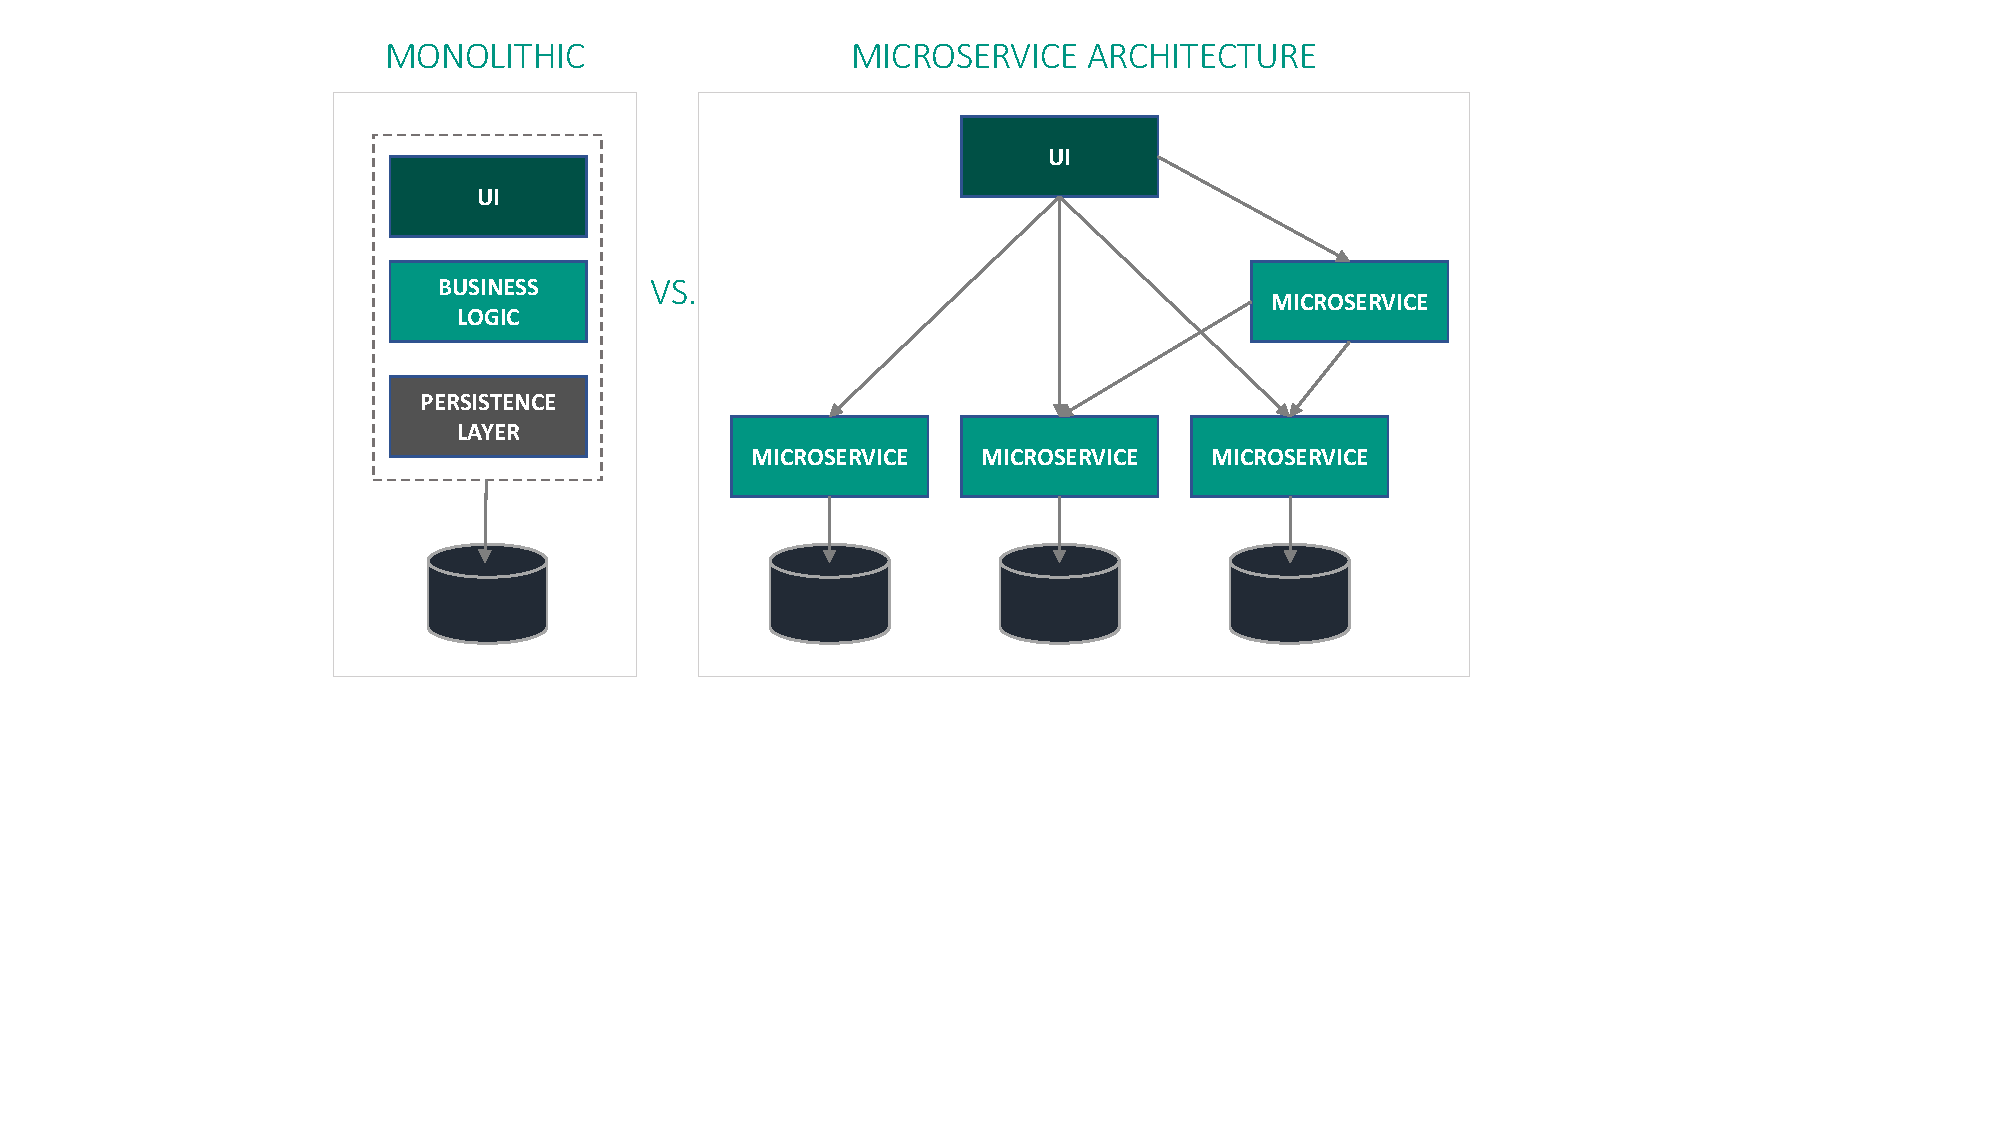
\includegraphics[width=\textwidth, trim={5cm 8cm 8cm 3cm}]{img/Architektur.pdf}
	\caption{Monolithic vs. Microservice Architecture}
	\label{fig:architekturMonolithVsMS}
\end{figure}

\subsection{Definition}
Yet, the term microservices is not formally defined in academia. A popular definition of microservices is  "a collection of cohesive and loosely coupled components, where each service implements a business capability"\cite{ObjectAwareAmiri}.
Amiri introduces three principles upon which the architecture is build: \textit{Bounded Context, Size, Independence} \cite{ObjectAwareAmiri}. \\
The first principle is about related functionality, that is combined in a single business capability - the  \textit{bounded context} \cite{FunctionalDecompositionHeinrich}. Each capability is implemented by one microservice. 
The \textit{Size} of a microservice is defined by the number of features it provides (namely bundled functional capabilities)  \cite{WorkloadbasedClustering}. There is no consensus about the "proper" size of a microservice \cite{DomainEngineeringMunezero}, but several guidelines exists: Services should focus on one business capability only \cite{ObjectAwareAmiri}. Others state, that the size of a microservice should not exceed a level, where it cannot be rewritten within six weeks \cite{WorkloadbasedClustering}. However, the sizes vary from system to system \cite{FunctionalDecompositionHeinrich} and even different sizes for each microservice in a specific system are possible \cite{DomainEngineeringMunezero}. The bottom line of \textit{Independence} is in Amiri's description of microservices as "a collection of high cohesive and loosely coupled components" \cite{ObjectAwareAmiri}. High cohesive services implement a relatively independent piece of business logic (at the most one business capability). Further, microservices should hardly depend on each other, which is the idea of being loosely coupled \cite{DataflowDrivenChen}.\\
Communication between microservices is achieved by lightweight message passing mechanisms such as \textit{REST}. Each service exposes a well defined interface (\textit{API}) with endpoints that provide information using standard data formats \cite{FunctionalDecompositionHeinrich}. 
The design of microservices mainly follows the \textit{Single Responsibility Principle (SRP)}: Each service should not have more than one reason to change \cite{TowardsUnderstandingEvolution}. The SRP mainly corresponds to the idea of not implementing more than one business capability.
The following covers the benefits and challenges of the microservice architecture.





\FloatBarrier

\subsection{Benefits}
\textbf{Fast and Independent Deployment} \\
As a matter of fact, each microservice is deployed independently \cite{interfaceAnalysisBaresi}. Changes to the code do not result in a full redeployment of the entire application \cite{FunctionalDecompositionHeinrich}. Consequently, software developers are able to react much quicker to changes in business requirements. This includes an acceleration in error correction. Per contra, any changes in a monolithic code base require a time consuming build of a new version and the redeployment of the entire application \cite{Fowler}. \\

\noindent
\textbf{Availability, Resilience and Fault Isolation} \\
Microservices are designed to operate independently of each other and to tolerate failure of services \cite{Fowler}. Large parts of the application remain unaffected of partly failures and the availability of the system is, at least partly, guaranteed. Monolithic application do not provide this type of fault isolation. If a failure occurs, the whole application remains unavailable as it is usually running in a single process \cite{ExtractionMazlami}. \\
 
\noindent
\textbf{Scalability and Resource Utilisation} \\
Small and independent microservices allow more fine-granular horizontal scaling \cite{WorkloadbasedClustering}. Single services can be duplicated to cope with changing workload during runtime \cite{DataflowDrivenChen}. Thus, dynamic (de-)allocation of resources on demand prevent infrastructure from being idle \cite{HeuristicsAlwis}. Scaling monoliths can only be attained by duplicating the entire application, leaving resources unused \cite{ClassificationOfRefactoring}. Further, each microservice is deployed on the best suitable infrastructure for its needs, allowing a more efficient system organization \cite{infoq}. \\

\noindent
\textbf{Improved Productivity} \\
In traditional software development, teams are divided based on their expertise: Database architects, UI-developers and server-side engineers, resulting in a three-tiered application (cf. Sec.\ref{sec:background:monolith}). Additionally, software engineers are responsible for the development only. Deployment is part of the operations team. This team structure results in high communication overhead and slows down the productivity \cite{Mazlami}. \\
In contrast, microservices are organized around business capabilities and require cross-functional, independent teams \cite{ObjectAwareAmiri}. Each team has the full range of skills required for the end-to-end realization of a microservice, including UI-development, database architecture, back-end engineers and project management. 
This minimizes the communication and interaction between the teams and thus, speeds up the productivity. Ultimately, microservices enable a more agile flow of development and operation \cite{ClassificationOfRefactoring}, also referred as \textit{DevOps}. 
\\


\noindent
\textbf{Neutral development technology} \\
Microservices are highly decoupled from each other, as they use standardized and lightweight communication mechanisms such as REST \cite{FunctionalDecompositionHeinrich}. Microservices can be realized using different programming languages, technologies and even deployment environments \cite{DataflowDrivenChen}. Developers are consequently not longer limited to use a single technology for the whole application. They can choose the most appropriate technology for each particular business problem or try out some new technology without rewriting the whole application \cite{ServiceCutter} \cite{TowardsTechnique}. 
 



\subsection{Challenges}
The previous section provides a vast amount of benefits that come with microservices. However, microservices are not the panacea of software engineering. System developers have to face challenges that can mitigate the benefits as described previously. The challenges are described in the following. \\ 

\noindent
\textbf{Expensive Communication}\\
Microservice use network protocols such as \textit{HTTP} to communicate with each other. Compared to standard, inter process communication (\textit{IPC}) as used in monoliths, remote procedure calls a more expensive \cite{SystematicMappingStudyMicroservice}. As a consequence, applications experience a decrease in performance as network communication is generally slower than \textit{IPC}.\\

\noindent
\textbf{Technical Challenges}\\
Microservices require a high degree of infrastructure automation \cite{MigratingTowardsSurvey}. The benefits of fast and independent deployment cannot be utilized, if it has to be done manually. Dynamic (de-)allocation of resources when scaling individual microservices need a well defined and structured cloud environment \cite{MigratingCloud}. 
Besides, the distributed microservice landscape complicates the logging mechanisms and performance monitoring \cite{SystematicMappingStudyMicroservice}. Traditional centralized logging, as it is used in monolithic applications, is not longer applicable. Instead, a careful aggregation system to gather logging and monitoring data from each service is required.\\

\noindent
\textbf{Organizational Challenges}\\
The microservice approach needs the establishment of cross-functional teams \cite{Fowler}. Adopting \textit{Continuous Practices}, such as \textit{Continuous Deployment}, are essential for the success of a profitable microservice architecture. Therefore, closer collaboration between development teams, operational staff and management has to be established. In summary, a costly and time consuming restructuring process of the entire organization is required \cite{NikoProseminar}. \\



\noindent
\textbf{Data Consistency}\\
Distributed systems need to share data. Heinrich et al. propose two concepts for the database architecture \cite{FunctionalDecompositionHeinrich}: The first concept applies the basic idea of the microservice approach, as it splits the database into several parts. Each microservice has its own database which manages the entities that belong to the corresponding bounded context. Higher speed and horizontal scaling are facing data consistency issues. Data needs to be synchronized which leads to inconsistency, if services are unavailable. The second concept is about sharing a single database. This approach overcomes the issue of consistency, as data is stored centrally. But sharing results in a loss of independence. Scaling can only be achieved through replicating the whole database. Research revealed, that the first concept is preferred \cite{FunctionalDecompositionHeinrich}. \\



\noindent
\textbf{Decomposition}\\
Decomposing a system into microservices is a very complex task that requires experienced system architects and domain experts \cite{Fowler}. It is irrelevant whether an existing system is decomposed into microservices or whether a new system is designed as a microservice-based application. The effort is very high in both cases.\\
Identifying the right granularity of microservice is one of the key issues. Too fine grained services cause inefficiency due to a high amount of expensive inter-service calls \cite{DomainEngineeringMunezero}. Developing the basic communication infrastructure adds additional complexity and slows down the initial developing process \cite{infoq}. \\



\section{Use Cases}
\label{sec:PrepApproach:UC}
Use Cases are a widely adopted technique to document software system requirements. Generally, they describe the interaction between actors (usually system users) and the software system itself. In this thesis, use cases are provided as semi-structured tables (following the notation presented by Cockburn et al. \cite{Cockburn}). \\ An example is given in Table \ref{tab:exampleUseCase}: Each use case has a unique identifier and a short description, followed by necessary preconditions and a trigger that causes the execution. The standard process is the main part and describes the success steps of the Use Case. Extensions provide additional information like alternatives or exceptional processes that occur in case of an unsuccessful step. 




\begin{table}[!h]
	\centering
	\begin{tabularx}{\textwidth}{|l||X|}
		\hline
		UC 5 & Show Stock Reports \\ 
		\hline
		Brief Description &  The opportunity to generate stock-related reports is provided
		by the Trading System. \\
		\hline
		Precondition & The reporting GUI at the Store Client has been started. \\
		\hline
		Trigger & The Store Manager wants to see statistics about his store. \\
		\hline
		Postcondition & The report for the Store has been generated and is displayed on
		the reporting GUI. \\
		\hline 
		Standard Process &
		
		1. The Store Manager enters the store identifier and presses the button Create
		Report.  \\
		& 2. A report including all available stock items in the store is displayed. \\  
		\hline
		Extensions & (none) \\ \hline
		
		
	\end{tabularx}
	\caption{Example Use Case in Tabular Form, Source: \cite{CoCoMEOld}}
	\label{tab:exampleUseCase}
	
\end{table}

\noindent
Besides being a widely adopted technique to specify system requirements, the textual use case notation is understandable without further technical knowledge. Neither previous knowledge in specific graphic notations like UML, nor the capability to create a complex domain model is necessary. Consequently, all sort of stakeholders (non-technical and technically experienced) are capable to provide the necessary information in terms of use cases. \\
However, the transformation into business models as presented in Sec.\ref{sec:PrepApproach:TransformUCtoBPMN} is not always trivial and requires some manual effort to produce high quality business processes. Nevertheless, it is necessary as the system requirements of the running example are given in form of textual use cases.





\section{Business Process and Model Notation}
\label{sec:PrepApproach:BPMN}
The Business Process and Model Notation (BPMN) is a graph oriented language to describe business processes. Originally, BPMN was designed to describe activities and their control flow dependencies only \cite{VisualizeBPMN}. Since the introduction of BPMN 2.0, it is possible to model the data needs and the data results of activities \cite{OMG}. Consequently, BPMN is capable to express the control flow and to approximate the data flow of business processes \cite{DataFlowErrorBPMN}. In the remainder, we use BPMN and BPMN 2.0 interchangeably. \\
BPMN is easy-to-use, powerful and widely adopted in academia and industry. Hence, BPMN is a suitable approach to extract the implicitly given data flow and control flow in the use case description. Sec.\ref{sec:PrepApproach:TransformUCtoBPMN} introduces a formal approach to generate BPMN processes from use case sets. Next, the BPMN 2.0 process definition is shortly introduced:

%"l, b, r, t"
\begin{figure}[h!]
	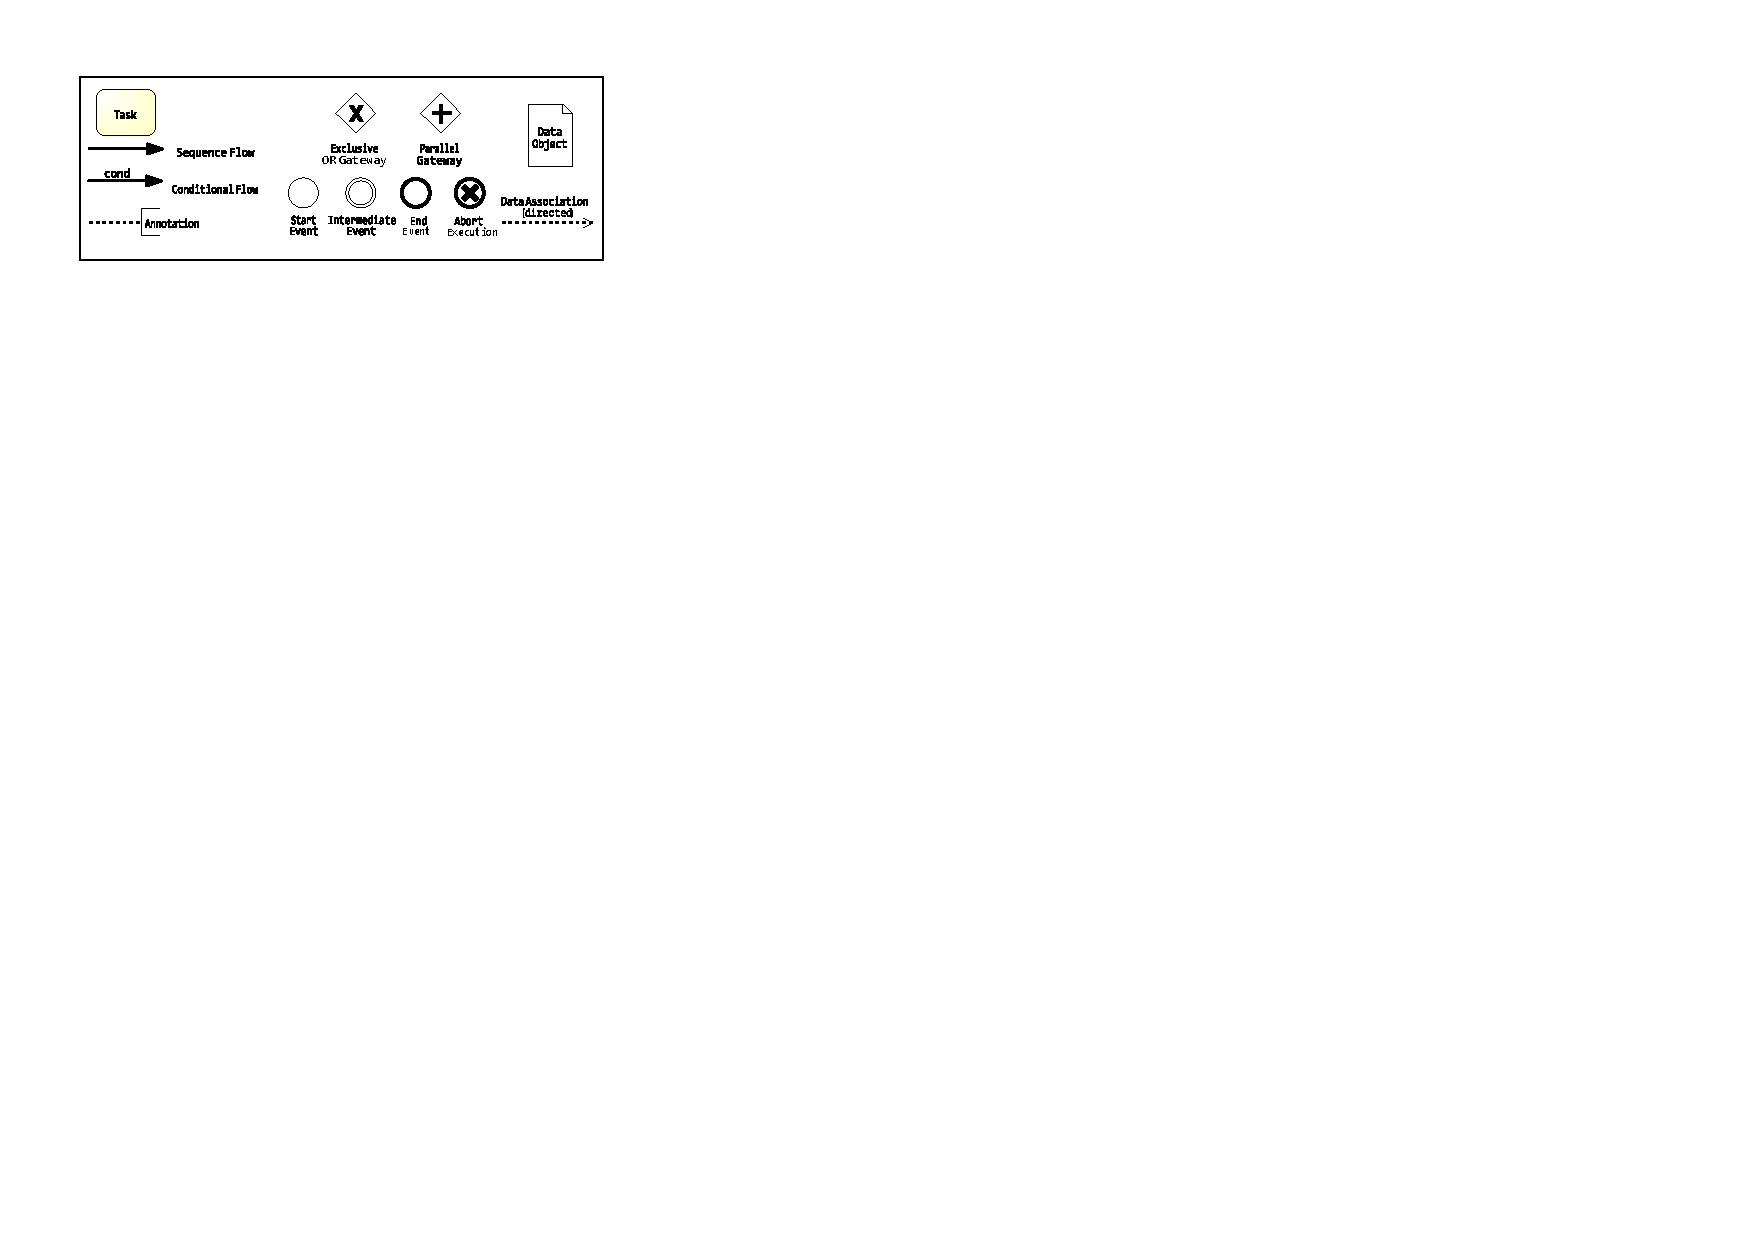
\includegraphics[width=\textwidth, trim={1cm 16.8cm 19.5cm 1cm}]{img/Overview.pdf}
	\caption{BPMN Notation (Subset)}
	\label{fig:BPMNSubset}
\end{figure}

\noindent
Fig.\ref{fig:BPMNSubset} presents the subset of BPMN symbols, that is required for the approach presented in this thesis \footnote{The entire specification is available at https://www.omg.org/spec/BPMN/2.0/}. Control flow activities are modelled as atomic \textit{Tasks} and connected through \textit{Sequence Flow Arcs}. \textit{Conditional Flow Arcs} integrate decision points into the control flow. Navigation decisions are based on the conditions related to the individual arcs. Such decision point are the \textit{Exclusive Or Gateway} and the \textit{Parallel Gateway}. Regarding the first one, if one of the incoming flows is triggered exactly one outgoing flow is activated based on the condition. For the latter, all outgoing flows are activated as soon as all of its incoming flows are activated. Each BPMN process starts with a \textit{Start Event} and ends with an \textit{End Event}. In case of several branches (due to Gateways), stop events need to be placed to each end. \textit{Intermediate Events} mark any other events that occur during the process. The trigger for an event is modelled using the \textit{Annotation} symbol. The \textit{Abort Execution Event} extend the \textit{End Event} and marks the error-prone end of a business process. \\
When it comes to data, each \textit{Task} may or may not require and/or produce data. Directed \textit{Data Association Arcs} provide the opportunity to model data needs and data results. In case a task requires data, the corresponding \textit{Data Objects} are connected to the task with the arrowhead attached to the task. Producing data works in the opposite direction. \\









\chapter{CoCoME}
\label{ch:CoCoME}

\section{Introduction to CoCoME}
\label{sec:CoCoME:Introduction}


\chapter{State of the Art}
\label{ch:StateOfTheArt}
This chapter outlines the current state of the art regarding microservice identification.  Sec. \ref{sec:StateOfTheArt:LiteratureReview} presents the search strategy and several existing approaches (Table \ref{tab:overviewLiterature}) that deal with the identification of microservices. Thereupon, the approaches are further explained and finally compared on the basis of several criteria.

\section{Literature Review}
\label{sec:StateOfTheArt:LiteratureReview}
The approaches mentioned in table \ref{tab:overviewLiterature} are the result of an extensive literature research which was conducted using the digital libraries IEEE \footnote{http://ieeexplore.ieee.org }, ACM \footnote{http://portal.acm.org} and SpringerLink \footnote{http://www.springerlink.com }. The web search enginge Google Scholar \footnote{http://scholar.google.com} provided further approaches and general information. \cite{FunctionalDecompositionHeinrich} was provided by the supervisor of this thesis and \cite{ServiceCutter} was cited by various approaches, including \cite{interfaceAnalysisBaresi}. The following search string was used:

\begin{centering}
{\itshape
   ["identify" OR "identification" OR "migrating" OR "monolith" OR "decomposition" OR "decompose monolith"
  	OR "decompose"] AND  "microservice"  \\
  	   OR \\  "microservice"  AND ["identification" OR "transformation" OR "refactor"]
}
 
   
\end{centering}

\noindent
Table \ref{tab:overviewLiterature} presents the 8 most promising approaches regarding the criteria mentioned in table //TODO!!!!!!. Now, a short introduction to each approach is given.




\begin{table}[h!]

\centering
     
	
	 \rowcolors{2}{gray!25}{white}
	\begin{tabularx}{\textwidth}{lXXlX}
		\rowcolor{gray!50}
		Link & Titel & Author   & Origin & Search String  \\
		
		\rowcolor{gray!50}
		& & (Year) & & \\
		
		\cite{ExtractionMazlami} & Extraction of Microservices from Monolithic Software Architectures  & G. Matzlami et. al. (2017) & Google Scholar&  {\itshape microservice identification }  \\
		
		
		\cite{ObjectAwareAmiri} & Object-Aware Identification of Microservice & M. J. Amiri (2018) & IEEE & \textit{identification microservices}\\\
		
		\cite{interfaceAnalysisBaresi} & Microservices Identification Through Interface Analysis & L. Baresi et. al. (2017)& SpringerLink & \textit{microservice identification}\\
		
		
		
		 
		 \cite{FunctionalDecompositionHeinrich}& Identifying Microservices Using Functional Decomposition & S. Tyszberowicz et. al. (2018) & \textit{provided} & \textit{n/a} \\
		 
		 \cite{DomainEngineeringMunezero} & Partitioning Microservices: A Domain Engineering Approach & I. J. Munezero et. al. (2018) & ACM & \textit{partition microservices}\\
		 
		 
		 \cite{DataflowDrivenChen} & From Monolith to Microservices: A Dataflow-Driven Approach & R.Chen et. al & IEEE & monolith microservice \\
		 
		\cite{HeuristicsAlwis} & Function-Splitting Heuristics for Discovery of Microservices in Enterprise Systems & A. De Alwis et. al. (2018 )& Google Scholar & identify microservices \\
		
	\cite{ServiceCutter} & 	Service Cutter: A Systematic Approach to Service Decomposition& M. Gysel et. al. (2016) & \cite{interfaceAnalysisBaresi} & \textit{n/a} \\
	
	\end{tabularx}
	\caption{List of authors and approaches}
	\label{tab:overviewLiterature}
\end{table}


\clearpage





\section{Approaches}


\noindent
\textbf{Extraction of Microservices from Monolithic Software Architectures   } \\
The approach presented in \cite{ExtractionMazlami} is a class based extraction model, that uses (meta-)information of a version control system \textit{(VCS)} such as Git\footnote{https://github.com/} to identify microservices. The approach is divided in two phases: The \textit{Construction Phase} and the \textit{Clustering Phase}.
Starting with a given code base, the approach uses three different coupling strategies and the information provided by the \textit{VCS} to transform the monolith into a weighted graph. Here, the nodes represent classes, and the edges have weights according to the chosen coupling strategy. In the second phase, a clustering algorithm determines possible microservices (each cluster is a microservice candidate). \\

\noindent
\textbf{Object-Aware Identification of Microservice  } \\
\cite{ObjectAwareAmiri} identifies microservices from business processes, using the widely known \textit{Business Process and Model Notation (BPMN)}. The activities in a business process represent functionality in the system. They also perform read and write operations on data objects. The goal is to identify microservices by using the structural and data object dependencies of the business processes. Therefore, the author proposes a clustering technique


\cite{ObjectAwareAmiri} uses clustering based on structural dependency and data object dependency. The system is modelled 





The approach models a system as a set of business processes using the well known graphical representation 
\noindent
\textbf{Microservices Identification Through Interface Analysis   } \\


\noindent
\textbf{Identifying Microservices Using Functional Decomposition  } \\


\noindent
\textbf{Partitioning Microservices: A Domain Engineering Approach } \\


\noindent
\textbf{From Monolith to Microservices: A Dataflow-Driven Approach } \\

\noindent
\textbf{Function-Splitting Heuristics for Discovery of Microservices in Enterprise Systems  } \\


\noindent
\textbf{Service Cutter: A Systematic Approach to Service Decomposition  } \\




\chapter{Preparation of Approach}
\label{ch:PrepApproach}









%TODO Nochmal drüber lesen kommt das in die DIscoussion?!


\section{Control Flow and Data Flow in BPMN Processes}
\label{ch:PrepApproach:ControlDataFlowBPMNProcess}
 


\subsection{Extract Data Flow of BPMN Processes}

As previously described, BPMN is only capable to express the data needs and the data results of single activities, whereas the data flow describes the flow of data in a process. By way of Fig.\ref{fig:restoreDataFlow}, \textit{Step 1} reads \textit{Data Object 1} and writes \textit{Data Object 2}. Despite the information about the data reads and writes of \textit{Step 1}, it is not possible to determine without further knowledge, if any information of \textit{Data Object 1} is used to write into \textit{Data Object 2}. Usually, this information has to be provided by system experts. \\
However, the approach presented in this thesis aims to reduce the required expertise or at least the additional information that is necessary when applying the approach. 
As a consequence, it is fundamental to approximate the data flow based on the data needs and writes of each activity. The approximation of the data flow works similar to the previous process. First of all, control flow related parts like sequence flows arcs, gateways, events and triggers are deleted. The remaining parts are tasks, data objects and data associations. Now, the tasks are not connected to their previous neighbours, with which they might exchange data, where the data exchange is synonymous with the flow of data.
To re-establish the possible data flow, follow the previously deleted control flow and reconnect the tasks with data association arcs by applying the following rules:












\chapter{Solution}
\label{ch:Solution}
This chapter presents the solution to tackle the issue of microservice identification. 
As noted in the \textit{State of the Art} chapter \ref{ch:StateOfTheArt}, existing approaches support two initial situations: They either conduct the extraction of microservices from existing (monolithic) systems or they are based on microservice greenfield development. Both types have their advantages and disadvantages. Existing systems, for instance, provide more information about the system specification and requirements. Legacy code and log files can be used to extract data dependencies or process structures. However, shortcoming in the design of the legacy application might have an impact on the extracted information and influence the microservice extraction in a negative manner. In contrast, greenfield development is not affected by any previously committed design decisions. As a matter of fact, the greenfield approach can be applied to existing systems as well by discarding legacy code and additional information that arose during the development. Solely the system requirements that existed before the implementation started serve as input. Nevertheless, this type has to manage the identification process with less input.\\
The solution we propose is based on pre-existing system requirements. No existing implementation is used and consequently, the presented approach is to be classified as greenfield method.\\



\section{Basic Approach}


\vspace{0.5cm}
\par
\begingroup
\leftskip=1cm
\rightskip=1cm

\noindent
\textbf{RQ1: Which is the most appropriate strategy to decompose a system into microservices? }

\endgroup
\vspace{0.5cm}



\noindent
This thesis proposes a formal, graph-based microservice identification approach using clustering on control flow and data flow. It is  inspired by Amiri’s work on \textit{Object-aware Identification of Microservices} \cite{ObjectAwareAmiri}. In chapter \ref{ch:StateOfTheArt}, eight suitable approaches to identify microservices are presented and compared using well-defined criteria. Most of them require special prerequisites and cannot be applied to various types of systems, i.e. no greenfield applications, systems without meaningful VCS meta-data or the absence of log files.
\\
By the way of contrast, Amiri proposes an approach to extract structural and data object dependencies from business point of view in order to generate possible microservice candidates. In doing so, he relinquishes to use any further information besides BPMN models. Using both, structural and data object dependencies promotes high cohesiveness and loose coupling on functional and data object level. In other words, high cohesive functionality is divided into the same microservices, together with the data objects that are accessed. \\
However, Sec.\ref{sec:stateOfTheArt:comparison} outlines the limitations and drawbacks of the approach. Whereas the control flow is depicted clearly, the data flow remains vague. The weight definitions regarding data object dependencies lack formal explanation. Further, the aggregation of structural and data object dependencies, and consequently the aggregation of control flow and data flow contains a significant problem: In Amiri's approach, the aggregation is conducted by summing up two relation matrices. The matrix entries representing the dependencies highly influence the results. For instance, a large amount of data reads and writes sum up to great numbers, outweighing the structural dependencies. Thus, the identification process would be almost based on data dependencies only, discarding any identified structural dependencies. \\
The following sections introduces a formal approach to tackle \textit{RQ2}. First, a basic overview of the approach is provided. Afterwards, each step is introduced in detail including alternatives and examples. 




\vspace{0.5cm}
\par
\begingroup
\leftskip=1cm
\rightskip=1cm

\noindent
\textbf{RQ2: What formal approach can be constructed to identify possible microservices without detailed know-how and manual effort? }

\endgroup
\vspace{0.5cm}



\noindent
To that end, Fig.\ref{fig:thesisProcess} provides an overview of the proposed approach. As depicted previously, the process requires input in form of BPMN models. Therefore, specifying those models marks the beginning of the process. Afterwards, control flow and data flow need to be extracted. To avoid the ambiguity of aggregating data flow and control flow as proposed by Amiri, the approach recommends to create two independent weighted Graphs, using the information from the previous step. In the next step, a clustering algorithm determines two sets of clusters based on the weights in the graphs. At that point, the process determined a set of clusters that is based on the control flow and another one, based on the data flow. In the following, a matching process identifies commonalities between data object-based and structural-based clusters in order to create comprehensive clusters. Based on these clusters, the last step extracts microservice candidates. \\
%TODO  stimmt das noch?
\textit{RQ2} also broaches the subject of necessary know-how and the amount of manual effort. As far as that is concerned, the proposed approach does not require human interaction as soon as the BPMN models are specified. Everything beyond that is based on a structural process.
Admittedly, the manual effort to conduct the process entirely is still not to be neglected, as the extraction process, graph creation and cluster matching is not yet automated. Nevertheless, the structural process enables to implement the entire approach, excluding the BPMN model specification step. However, implementing an approach is beyond the scope of the paper.




 
\begin{figure}[h!]
	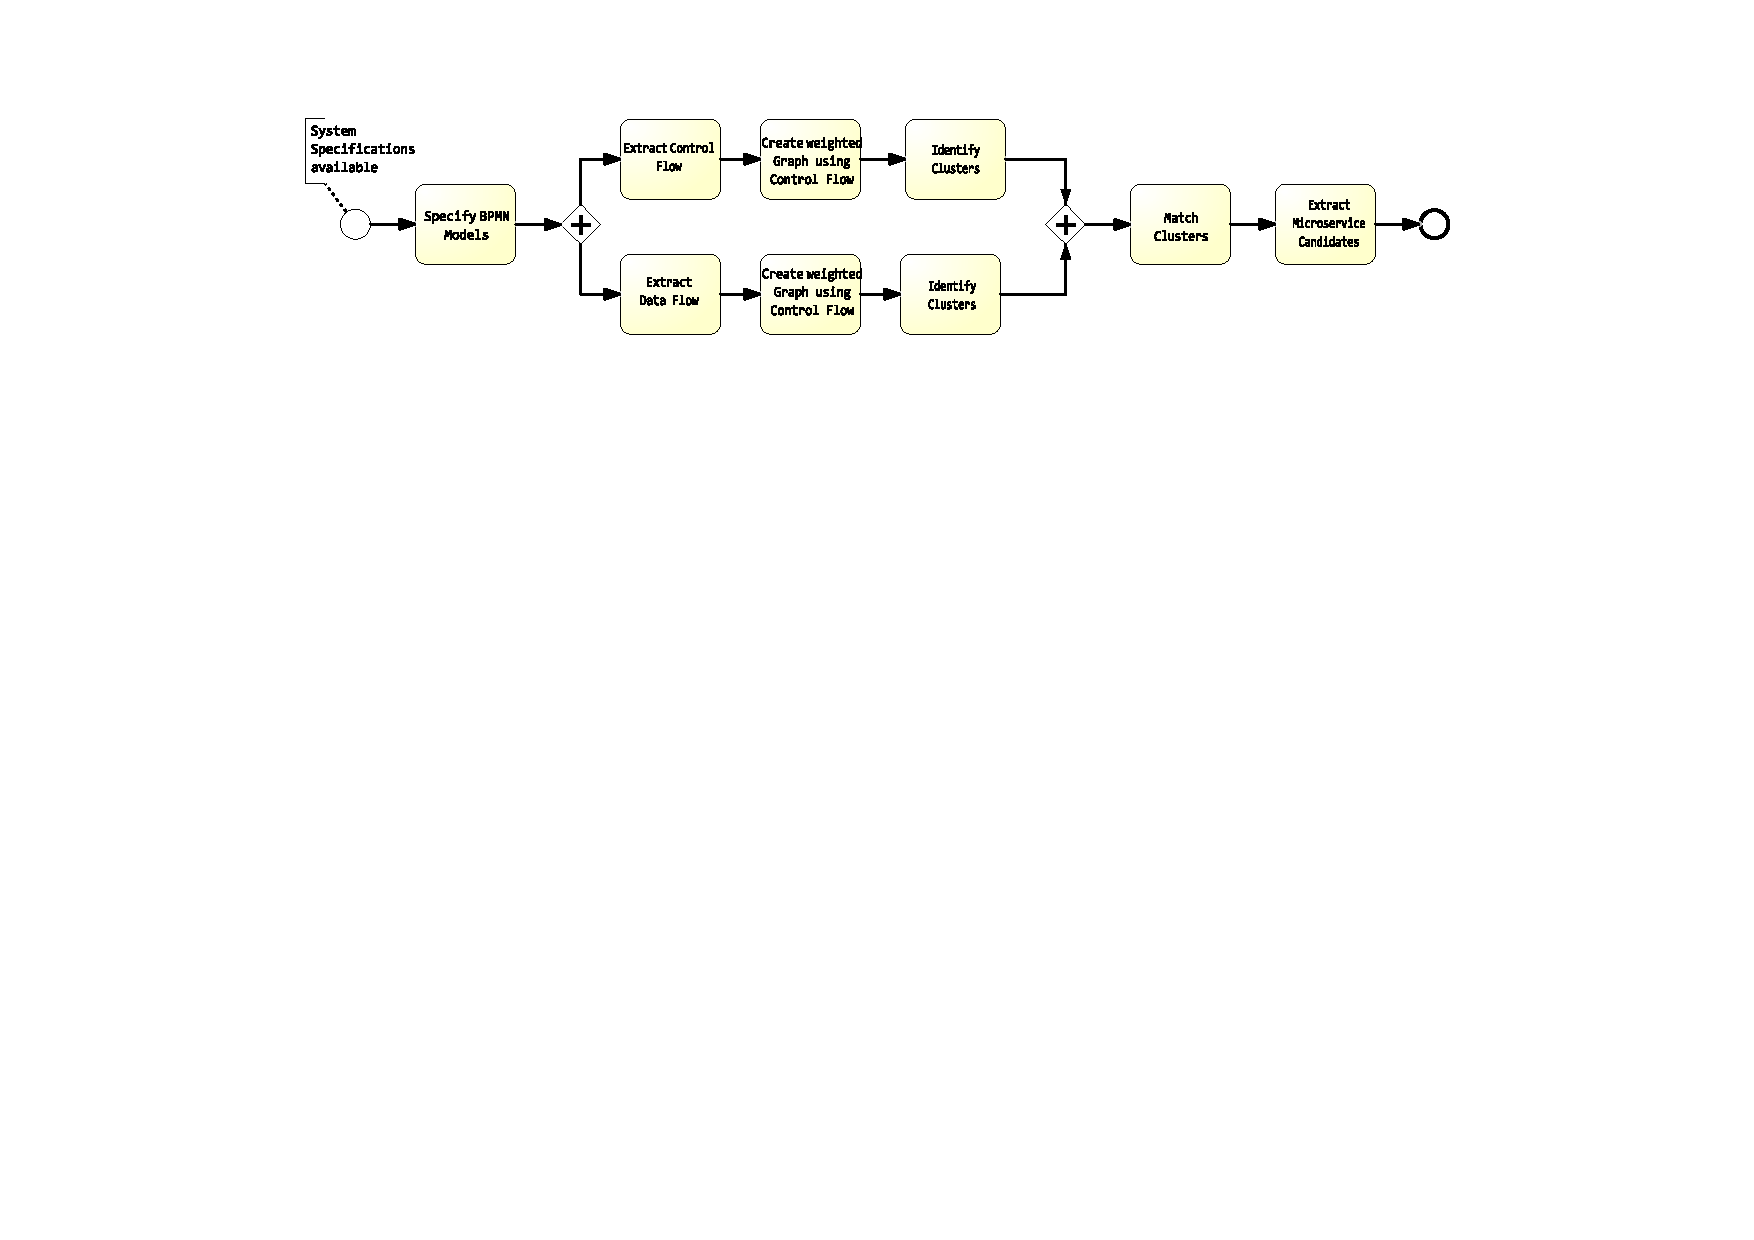
\includegraphics[width=\textwidth, trim={7.5cm 15.3cm 5.0cm 1.5cm}]{img/ThesisProcess.pdf}
	\caption{Overview of the identification approach}
	\label{fig:thesisProcess}
\end{figure}






\section{Specify BPMN Models}
\label{sec:Solution:SpecifyBPMN}
Chapter \ref{ch:PrepApproach}, introduces the BPMN 2.0 modelling language as an easy to use, but yet powerful notation to illustrate business processes including their activities and their data needs.
In the first step of the solution, those business processes need to be specified. Usually, the system specification are not directly given in form of business processes, bur rather in the form of use cases, UML models, domain models or even as textual description in natural language. Therefore, the first step consists of specifying a business model using the available system specification. This can be achieved using various approaches, for instance: \\

\noindent
\textbf{Workshops} At the very beginning of a software project, technical and non-technical stakeholders can participate in a workshop to specify the business process model. As illustrated in the BPMN specification, the "primary goal of BPMN is to provide a notation that is readily understandable by all business users"  \cite{OMG}. Therefore, carrying out a workshop with stakeholders from various departments can produce high quality BPMN models which can be further used as input for the extraction process.\\

\noindent
\textbf{Use Cases} In the case of CoCoME, the system specifications are available as use cases (cf. chapter \ref{ch:CoCoME}). Accordingly, section \ref{sec:PrepApproach:TransformUCtoBPMN} illustrates a process to transform use cases into BPMN models. 
\\

\noindent
\textbf{Others} Business processes can be extracted in various other ways. UML Activity diagrams, for instance, are very similar to BPMN models. Van der Aalst et al. elaborated the Process Mining Manifesto \cite{ProcessMiningManifesto} where he presents general techniques to extract business processes, although it is mainly event log driven. Another approach is the \textit{BPMN Miner}, an automatic discovery tool for BPMN process models \cite{BPMNMiner}. Again, the tool discovers the models dynamically, using log files of a legacy system.



\section{Extract Control Flow}
\label{sec:Solution:ExtractControlFlow}
In the course of the process, activities of the business processes are clustered based on their structural dependency which is extracted from the control flow. Activities (tasks) in business processes play the role of operations in microservices, representing the functionality a service is able to offer. During the process of microservice identification, it is desired to cluster high cohesive functionality into one microservice. To achieve this, one must first extract the structural  dependencies between activities in business processes. \\
The extraction process itself is trivial, as the business process language BPMN was designed to illustrate the control flow between activities (cf. Sec.\ref{sec:PrepApproach:BPMN}). Mainly inspired by the work of M. Amiri in \textit{Object-aware Identification of Microservices} \cite{ObjectAwareAmiri}, we propose a straightforward technique to separate the control flow information from BPMN 2.0 models in section \ref{ch:PrepApproach:ControlDataFlowBPMNProcess}. The control flow has to be extracted for each BPMN model that was specified in the previous step.




\section{Extract Data Flow}
\label{sec:Solution:ExtractDataFlow}
Besides the structural dependencies of activities, data object access plays a significant role in the definition of microservices. As depicted in the background chapter \ref{ch:background}, microservice generally administer their own database with the data entities that belong to the bounded context of the service. Usually, data needs to be shared among services which raises the question where to place a shared data object. However, sharing data among microservices is expensive because it includes network communication instead of inter process communication. It is therefore desirable to reduce the communication between services by distributing data objects into the same microservice if they are accessed together.  
Like the previous section, we propose to use clustering based on data flow to identify high cohesive but loosely coupled set of data object clusters. \\
When BPMN 2.0 was introduced, the language was extended by the ability to represent data objects that are consumed and/or produced by the activities. Despite the fact that BPMN is still a language to illustrate the control flow of business processes, the extension provides the possibility to visualize an approximated data flow based on the data needs and writes of each activity. In Sec.\ref{ch:PrepApproach:ControlDataFlowBPMNProcess}, we present a formal approach to extract the data flow by discarding anything but flow elements used to represent the data flow. Again, the data flow has to be extracted for each BPMN model that was specified in the previous step.



\section{Create a weighted Graph using Control Flow}
\label{sec:Solution:CreateGraphControl}
In section \ref{sec:Solution:ExtractControlFlow}, the control flow is extracted from several BPMN models that represent the entire system.
The visualization of the control flow information as a single graph enables to identify clusters of high cohesive functionality among all BPMN models, thus among the entire system. 
Therefore, we build a directed graph G whose vertices represent the tasks/activities in the BPMN models. Duplicate vertices are not allowed. Hence, activities that occur several times in different BPMN models are only represented once in the graph.
The edges correspond to the control flow arcs: a pair of activities is connected if there is a direct edge in the business processes or if there is a path between them that contains only gateways. This decision is based on the heuristic, that two activities are more likely to be in the same microservice, if they are directly connected in a business process. \\
Speaking of the weights, we decide to assign a value of 1 to each edge notwithstanding of the nature of the connection, which is i) directly connected ii) connected via parallel gateway iii) connected via XOR gateway. Regarding the first and the second case, it is motivated by the fact that activities connected by a parallel gateway and activities that are directly connected are always executed during control flow execution.
In regard of the third case, one can argue that the probability of a condition influences the weight of a connection. For instance, a task has two subsequent tasks that are connected through an exclusive OR gateway and conditional flows. One of the tasks, the "main task", is more likely to be the successor as the alternative. Hence, the edges need a different weight. However, the information regarding the probability is usually not available and specified in business processes. Further, different weighting raises the question of the value determination. With this in mind, the generalization of all types of connections (using a weight of 1 for all edges) seems to be an appropriate solution. \\
In the case of duplicated control flow dependencies due to several BPMN models, the weights are summed up as a pair of connected tasks that occurs in multiple models indicates a stronger cohesion. As a result, the edge in the graph that connects the tasks in questions receives a greater weight (corresponding to the number of occurrences).\\
Fig.\ref{fig:controlFlow} shows an exemplary BPMN process whose object-related information has already been deleted (cf. Sec.\ref{sec:Solution:ExtractControlFlow}). As explained in this section, the control flow information given in this BPMN model is used to create a weighted graph. The corresponding graph is illustrated in Fig.\ref{fig:controlFlowGraph}. 


\begin{figure}[h!]
	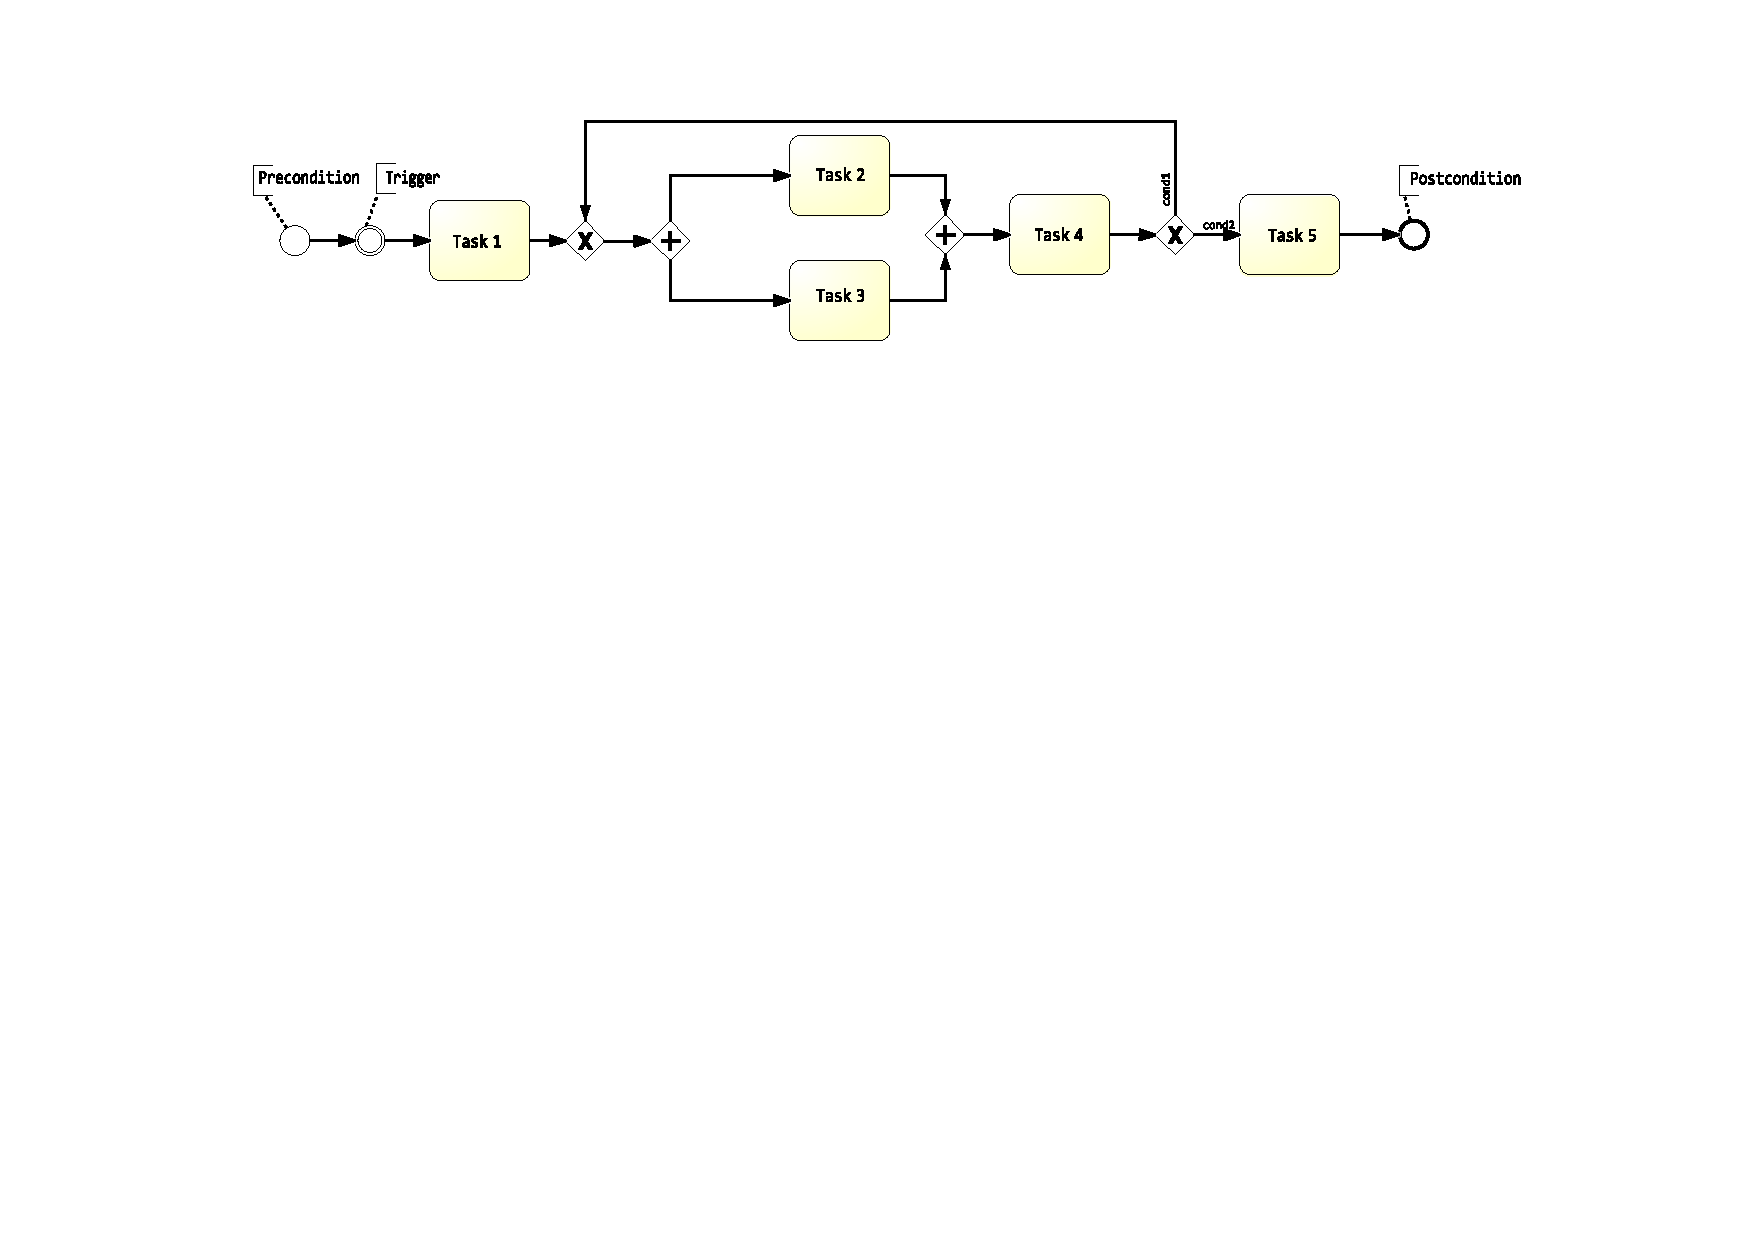
\includegraphics[width=\textwidth, trim={4.5cm 14cm 4.0cm 1.5cm}]{img/ControlFlowExample.pdf}
	\caption{An exemplary BPMN model illustrating the control flow only  }
	\label{fig:controlFlow}
\end{figure}
%"l, b, r, t"
\begin{figure}[h!]
	\centering
	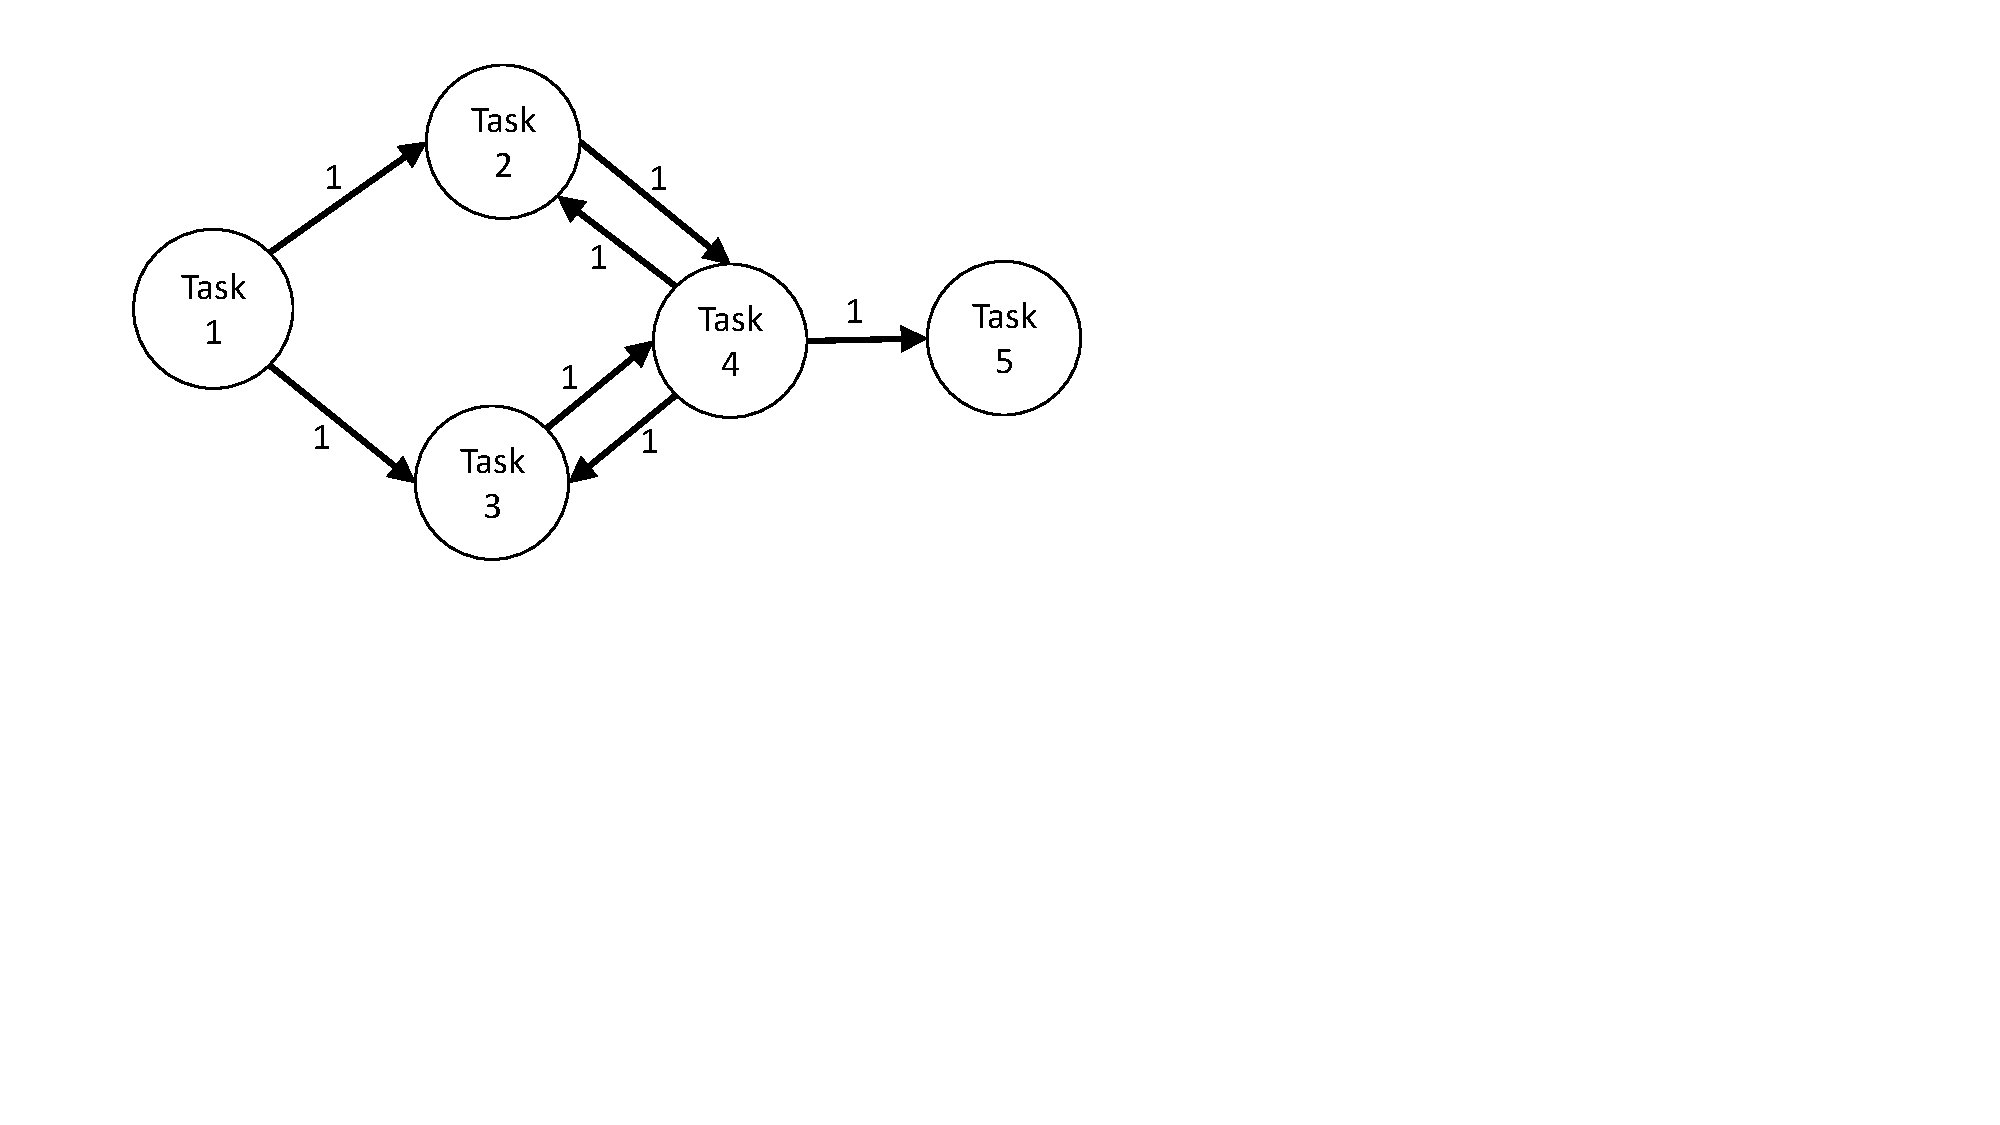
\includegraphics[width=12cm, trim={1.5cm 9.0cm 13.0cm 0cm}]{img/ControlFlowGraph.pdf}
	\caption{Weighted graph using Control Flow Dependencies}
	\label{fig:controlFlowGraph}
\end{figure}

 






\section{Create a weighted Graph using Data Flow}
\label{sec:Solution:CreateGraphData}
To identify high cohesive data object clusters, the data flow information is visualized as a weighted graph, which is similar to the activity graph as described in the previous sections. In this case, the vertices of a Graph G represent the data objects in the BPMN models. Like the activity graph, duplicated vertices are not allowed. Each data object is only represented once in the graph. The edges illustrate the data object dependencies extracted from the data flow. \\
Such dependencies are: i) data objects read by the same task ii) a data object value that is used when writing to (or creating) another data object. \\
Speaking of the first dependency, it is obvious that data which is read by the same task is more likely to be partitioned into the same service. Otherwise, the execution of a task would always cause at least one expensive intra-service call.
Therefore, two vertices that represent a pair of data objects which are read by the same task is to be connected by an edge. \\
The second dependency is based on a similar heuristic. There is a certain connection between two data objects, if information of one data object is used to update or create another one. Placing the information source into another microservice as the information destination would require an inevitable cross-service communication which is meant to be prevented. \\
To create a weighted graph based on data flow dependencies, it is necessary to take a closer look at the extracted data flow (cf. Sec.\ref{sec:Solution:ExtractDataFlow}). It is noticeable that it requires additional information to decide whether two data objects have one of the proposed connections. Fig.\ref{fig:dataFlowExample} represents an exemplary data flow diagram that was extracted from a BPMN process. In the following, we discuss different possibilities to gain the data object dependencies.


%"l, b, r, t"
\begin{figure}[h!]
	\centering
	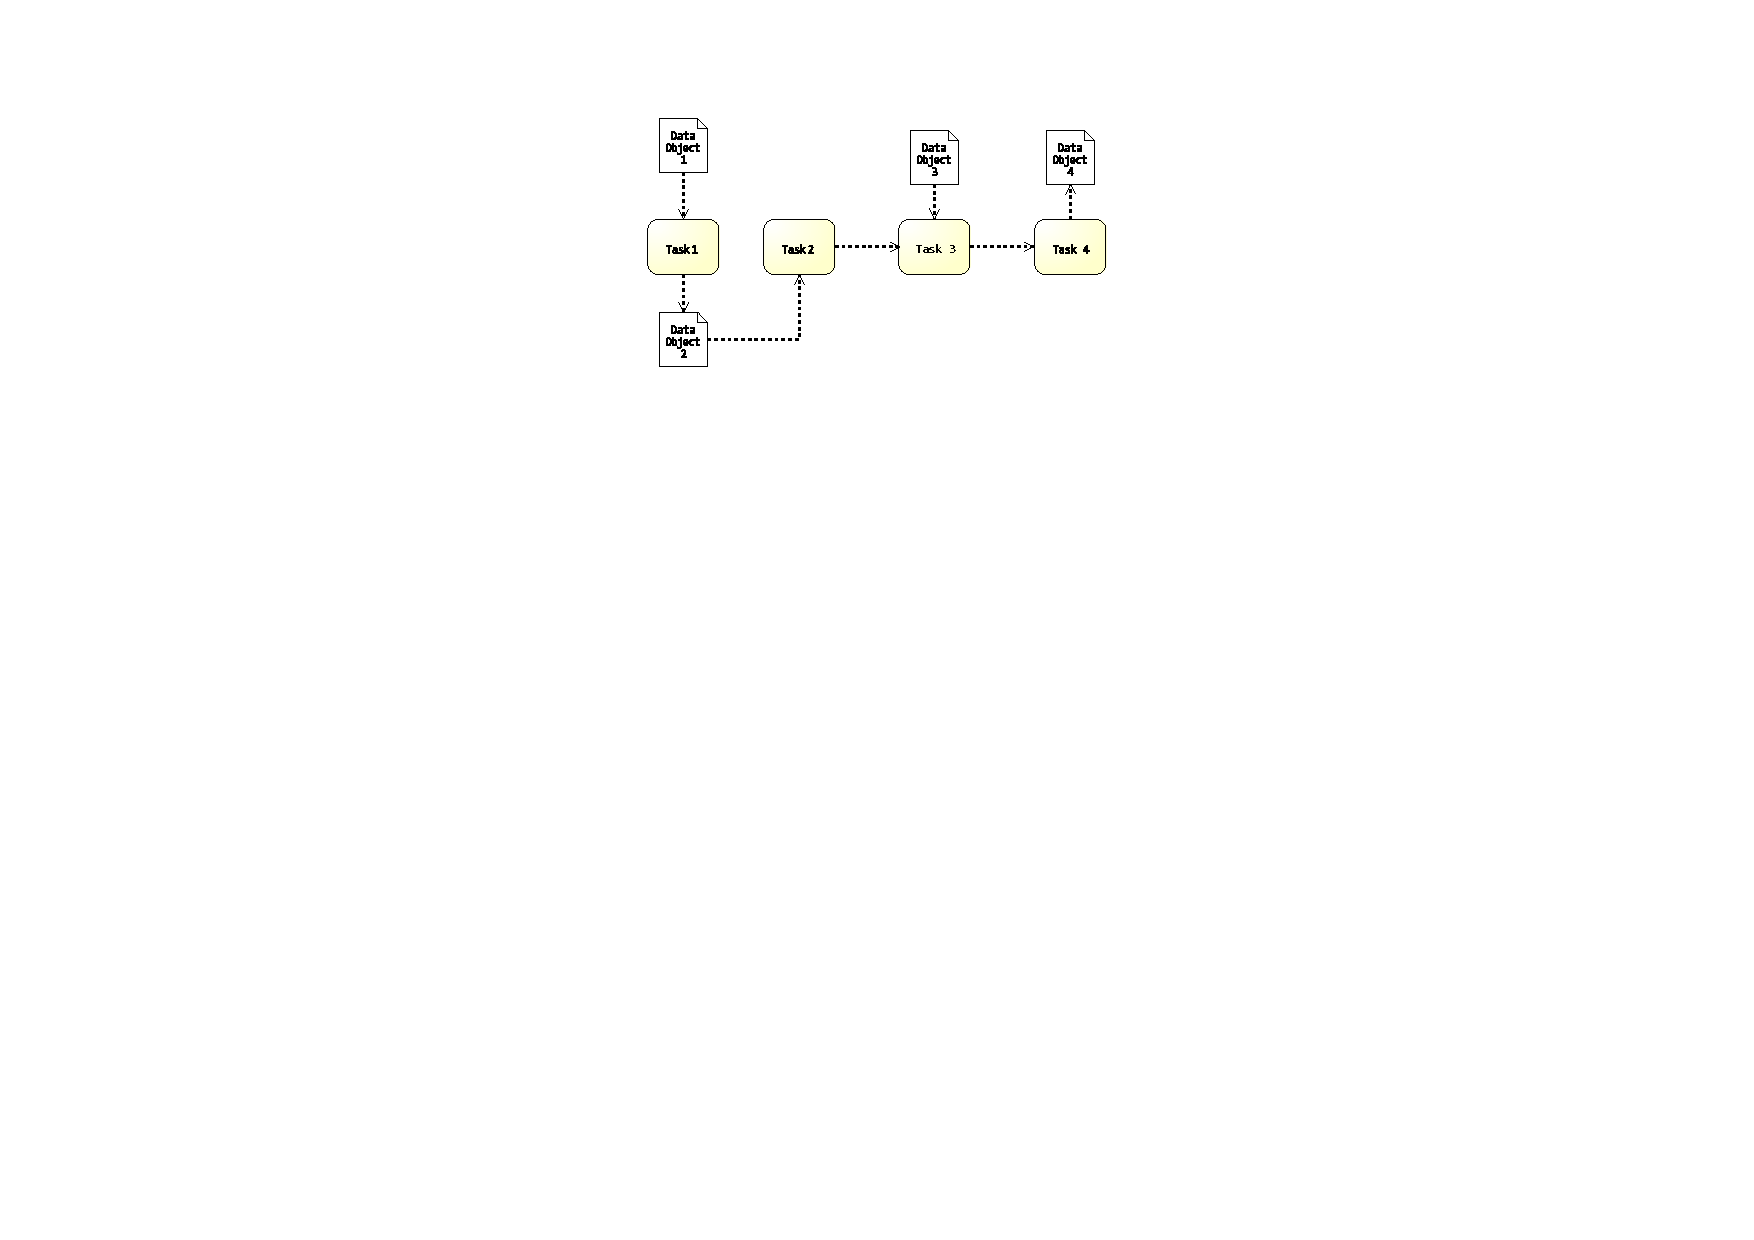
\includegraphics[width=\textwidth, trim={10cm 14.5cm 10cm 2cm}]{img/DataFlowExample.pdf}
	\caption{Data Flow Diagram extracted from BPMN process}
	\label{fig:dataFlowExample}
\end{figure}

Information of one data object can flow into another one. That is the case, if a data object is updated or created using information of another data object which was read beforehand. 
For instance, \textit{Task 3} processes information of \textit{Data Object 3}, passes it to \textit{Task 4}, which uses the information of the data object to update \textit{Data Object 4}. Consequently, \textit{Data Object 3 \& 4} should be connected by an edge in the resulting data object graph. Yet, another possibility is that \textit{Task 3} only reads \textit{Data Object 3} and displays some information to the user. Further, \textit{Task 4} only processes user input to update \textit{Data Object 4}. Hence, \textit{Data Object 3 \& 4} are not to be connected by an edge, as there is no information flow in between. \\
The same line of reasoning can be applied to \textit{Task 1}: Information of \textit{Data Object 1} may or may not flow into \textit{Data Object 2}, although both data accesses are executed by the same task. As a final point, the information of several data objects may flow into another one. For example, \textit{Data Object 2}, produced by \textit{Task 1} and \textit{Data Object 3}, read by \textit{Task 3}, may be used to create \textit{Data Object 4}.\\
Given these points, identifying data object dependencies has to be estimated. The following possibilities are available to estimate the data dependencies:


\begin{itemize}
	\item Dependency between a pair of data objects, only if both data objects are read and written by the same task.
	\item Dependency between a pair of data objects, if \textit{n} tasks\footnote{n $\in [0..]$, where 0 represents neighbouring tasks} are in between a task that reads the first data object and another task that writes into the other data object\footnote{Following the Data Flow Arcs when counting}.
	

	
	\item Use additional information to determine the actual data flow dependencies
\end{itemize}
\noindent
The dependencies are expressed by connecting the vertices in question (which represent the data objects) with a weighted edge. 
Obviously, the third possibility is the most accurate one. The identified data object dependencies correspond to the reality. Though, one of the thesis' goals is to reduce human involvement to a minimum, so that the approach is able to run without further user interaction. Consequently, this possibility is discarded. \\
Regarding the first option, data object dependencies are frequently underestimated, as no information flow from one task to another is discerned. For this reason, option one is also discarded. \\
With this in mind, the second option seems to be the most appropriate one to determine the data flow dependencies based on the data flow graph. Still, the number \textit{n} has to be defined. Having \textit{n=0}, only data objects that are processed by neighbouring tasks are considered to share a dependency, therefore connected by an edge. This is reasonably similar to the control flow dependency, where only neighbouring tasks are connected by an edge as well. However, we empirically examined the data flow with \textit{n=0} and experienced an underestimation of the existing data flow dependencies. This is due to the fact that data processing and data storing is quite often distributed among several tasks. Fig.\ref{fig:ExampleDataProcessing} illustrates an example: 


%"l, b, r, t"
\begin{figure}[h!]
	\centering
	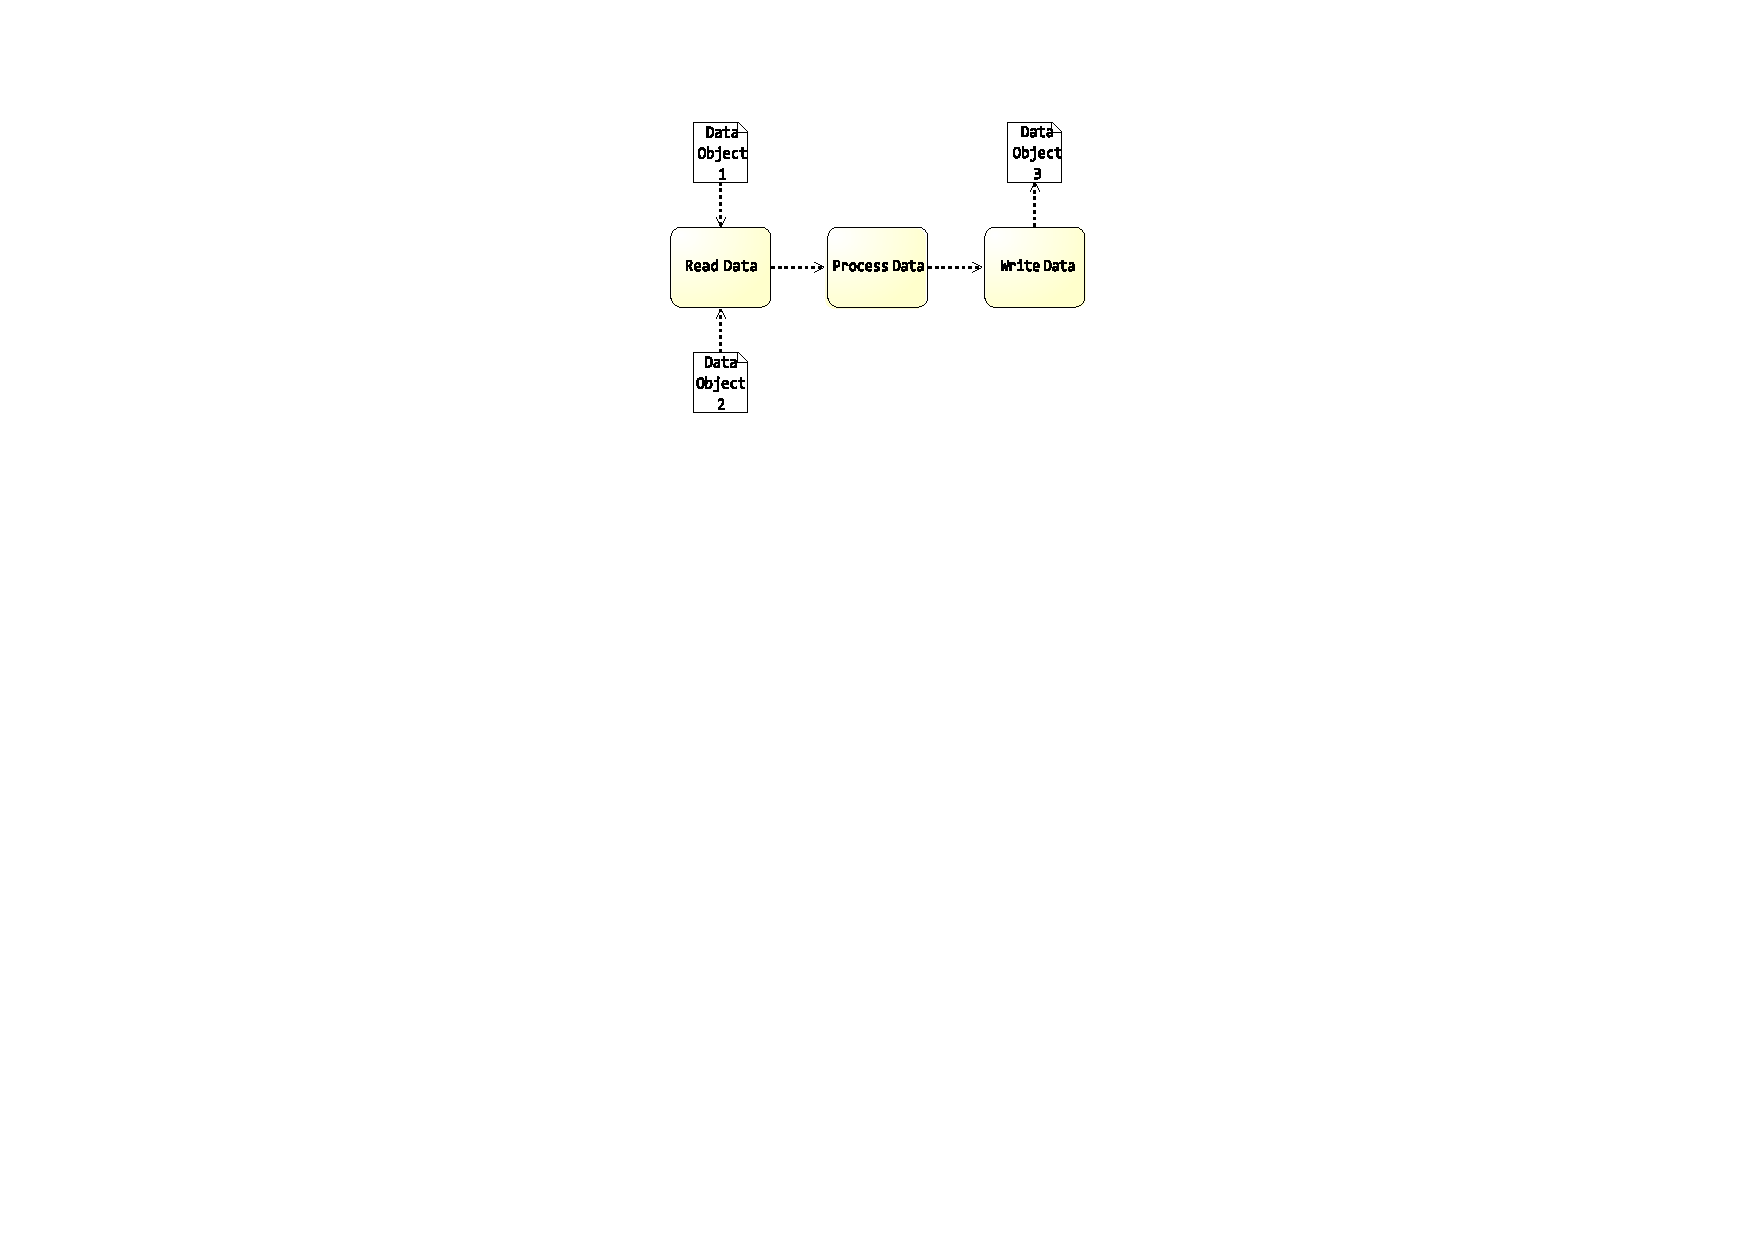
\includegraphics[width=11cm, trim={10cm 14.0cm 10cm 1.9cm}]{img/ProcessDataDFD.pdf}
	\caption{Data Flow Diagram to demonstrate data processing and data storing}
	\label{fig:ExampleDataProcessing}
\end{figure}

\noindent
Two data objects are read by the first task and passed to its neighbour, which is only in charge of processing it. Finally, the merged information is stored by a third task. To represent this common pattern of data processing, a value \textit{n>0} is required. \\
Nonetheless, reading and processing the data can be distributed among several tasks, depending on the granularity of the business processes. For instance, a more fine-granular business model divides the processing of \textit{Data Object 1} and \textit{Data Object 2} into two tasks, which still represents the same process.
Thus, determining the parameter \textit{n} highly depends on the granularity of the business processes. On the one hand, the value has to be big enough to cover data dependencies that are distributed among several tasks due to a more fine-grained process modelling. On the other hand, it should not be too big in order to prevent an overestimation of data dependencies due to data access which is executed by distant tasks. In our case, \textit{n=1} produced the best results. \\
Speaking of the weights, we decided to assign a weight of 1 to each each edge notwithstanding of the connection type, which again is i) two data objects are read by the same task ii) a data object value that is used when writing to another data object. Other approaches, like the one proposed by Amiri \cite{ObjectAwareAmiri}, often differentiate between data reads and data writes, where the latter is generally weighted higher. However, the cross-service communication outweighs the difference between both data access types. In detail, a cross-service data read is generally much more time consuming compared to a inter-service write, due to the expensive network communication. Consequently, we propose to generalize data accesses by considering binary data dependencies only: two data objects are dependent according to the rules mentioned previously or they are not. 
In the case of duplicate data flow dependencies due to several tasks across various BPMN models that process the same data objects, the weights are summed up. This is motivated by the fact that multiple appearances of the same data object dependencies indicate a stronger cohesion.
Fig.\ref{fig:dataFlowGraph} illustrates the Graph that is produced when applying the approach to the data flow described in Fig.\ref{fig:dataFlowExample}.






%"l, b, r, t"
\begin{figure}[h!]
	\centering
	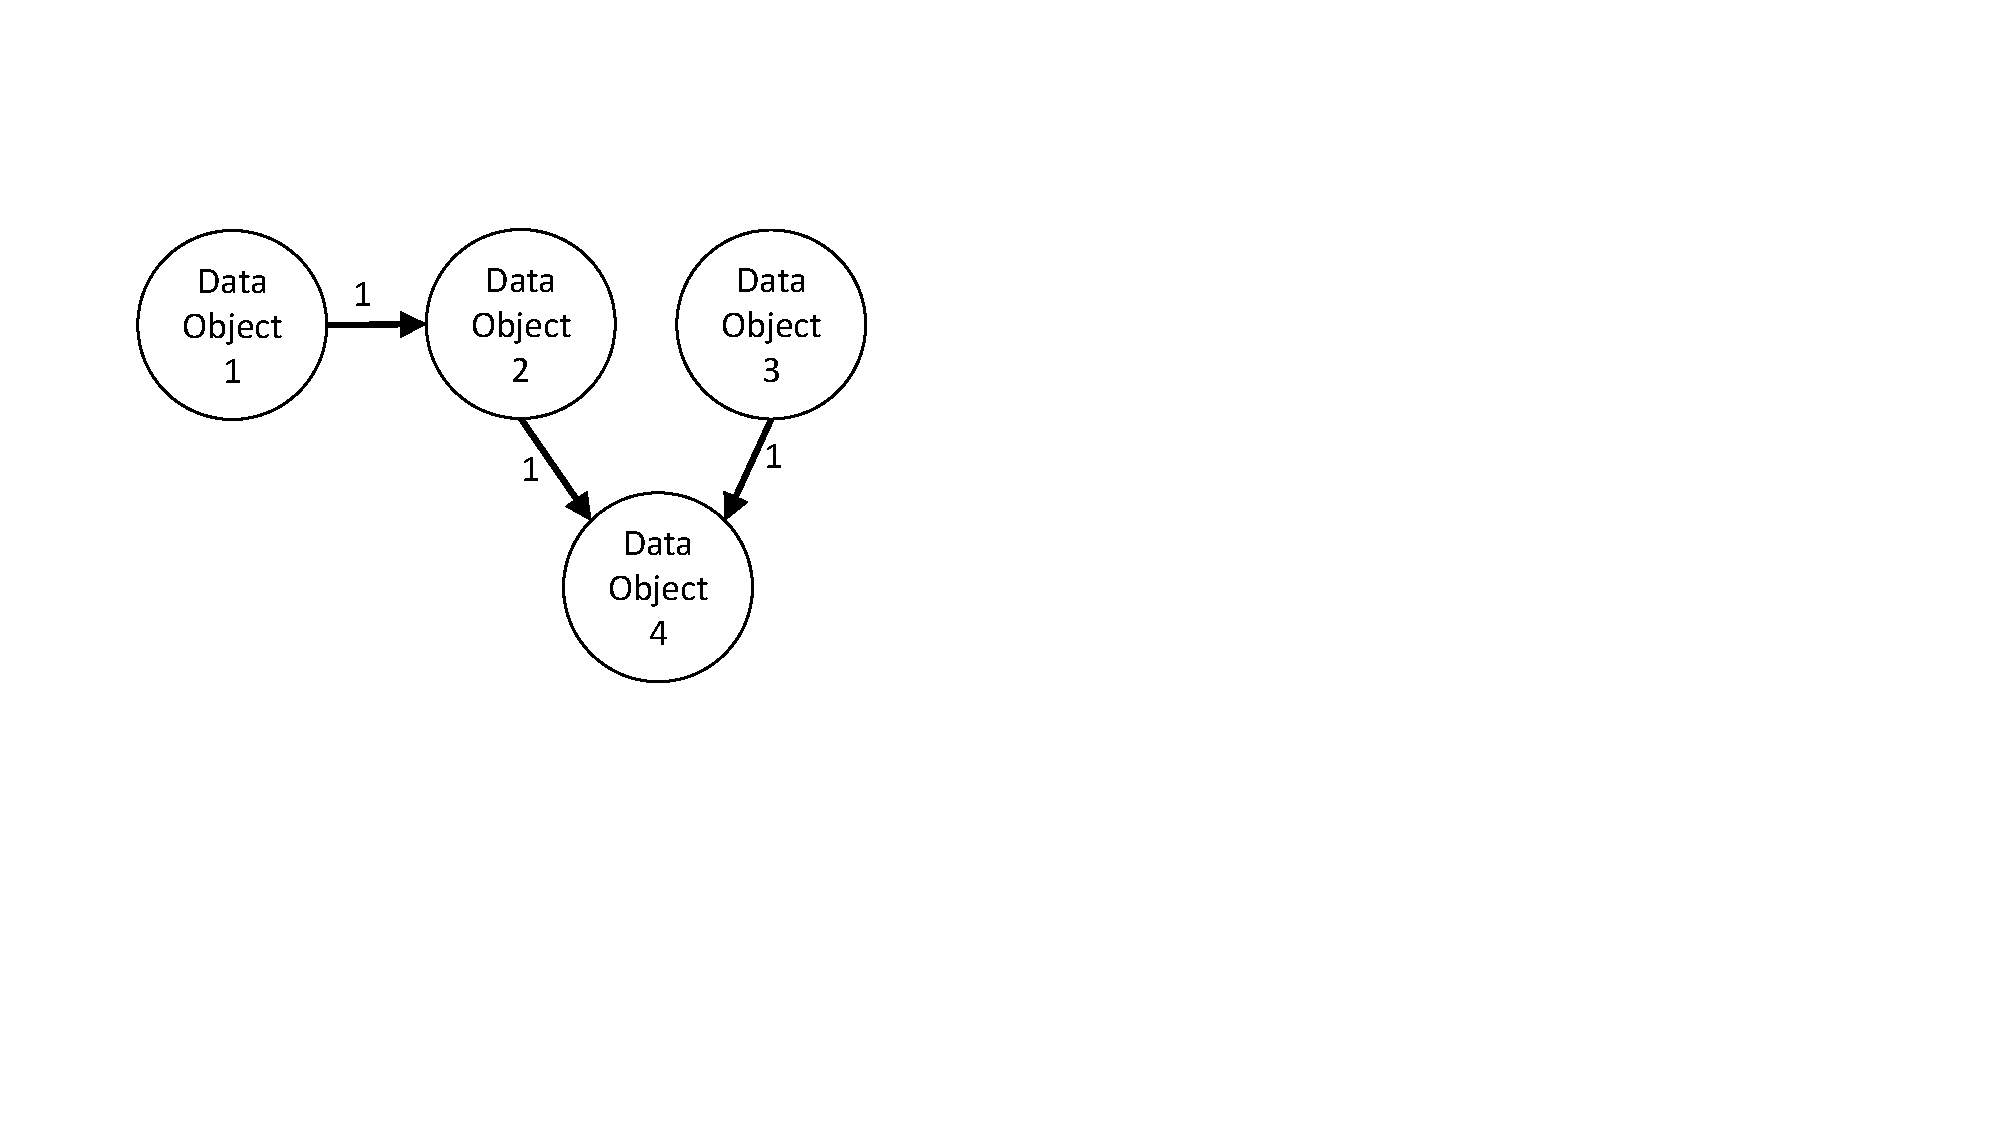
\includegraphics[width=10cm, trim={1.5cm 9.5cm 16.0cm 0cm}]{img/DataFlowGraph.pdf}
	\caption{Weighted graph using Control Flow Dependencies}
	\label{fig:dataFlowGraph}
\end{figure}


%"l, b, r, t" width=12cm, trim={1.5cm 7.5cm 13.0cm 2cm






\section{Identify Cluster}
\label{sec:Solution:IdentifyCluster}
The previous sections define strategies to represent the data flow and control flow dependencies as bi-directed weighted graphs. In this step of the identification process, the graphs are cut into disjunct set of nodes, called clusters. Common clustering techniques enable to identify sets of nodes with strong internal relationships and weak connections to the other clusters. The clustering is to be applied to both graphs equally, as they do not have any conceptual differences. At this point, it is important to emphasize that the elaboration of a clustering algorithm is beyond the scope of the paper. Therefore, we use existing tools for the visualization and identification of clusters. \\
In the course of this work, the first attempt to identify clusters involved the use of the graph visualization tool \textit{Gephi} \footnote{https://gephi.org/}. To layout the graph, the tool uses a force-directed algorithm based on gravity and repulsion called \textit{Force Atlas} \cite{gephi}. For the clustering, it uses a heuristic algorithm elaborated by Blondel et al. to find "high modularity partitions of large graphs" \cite{modularity}. Whereas the activity clustering produced continuously constant results, the data object clustering did not. Despite using the same settings, the tool produced fair different sets of clusters when executing the algorithm. Obviously, the tool is not suitable for relatively small graphs as in the case of CoCoME.  \\
Upon further research, we choose a tool called \textit{Bunch}, which is a clustering tool that creates a graph decomposition by treating clustering as an optimization problem \cite{bunch}. \textit{Bunch} uses a genetic algorithm and a fitness function called \textit{Turbo-MQ} \cite{turbo-MQ}. In each iteration, the algorithm randomly picks \textit{K} clusters and calculates \textit{Turbo-MQ} to measure the fitness of the selected partition. In the next iteration, the algorithm tries to improve the fitness by making changes to the previous selected clusters. The algorithm stops, as soon as the overall fitness converges.\\
Mitchell et al. defined the "modularization quality \textit{MQ} measurement" \cite{turbo-MQ}, in such a way, that it rewards intra-cluster coupling while penalizing inter-cluster coupling:

\vspace{1cm}
\noindent
\begin{minipage}{.25\linewidth}
	
	\flushleft
	\begin{math}
	  Turbo-MQ = \sum_{i=1}^{k} CF_{i} 
	\end{math}
	

\end{minipage}%
\begin{minipage}{.5\linewidth}
	\flushleft
	\begin{math}
      CF_{i} = \begin{cases}
       0 & \mu_{i} = 0 \\
        \frac{\mu_{i}}{\mu_{i} + \epsilon_{i}}  & otherwise
      \end{cases}
  \end{math}


\end{minipage}
\vspace{1cm}


The \textit{MQ} value of a partition with \textit{k} clusters is calculated by adding the \textit{Cluster Factor (CF)} of each cluster. $CF_{i}$ describes the normalized ratio between the total amount of internal edges $\mu_{i}$ and the amount of edges $\epsilon_{i}$ that originate in cluster \textit{i} and end in another cluster. The \textit{CF} value is between 0 (no internal edges) and 1 (no edge to another cluster), where larger values indicate a better quality of the partition. \\
Bunch requires the input graph in a simple textual form: The Graph is represented as list of edges, where each edge is described in a separate row by \textit{<start node>} \textit{<end node>} \textit{<weight>} (without the pointed brackets). The output is in the \textit{DOT} format \cite{DOT}, which is a powerful graph description language. To visualize the clustered graph, we use the open-source tool \textit{Graphviz} \footnote{https://www.graphviz.org/}.




\section{Match Cluster}
\label{sec:Solution:MatchCluster}
Having both sets of clusters, it is now necessary to match the activity clusters and the data clusters in a way that reduces the required inter-microservice communication. As a first step, it is necessary to count how many times an activity cluster accesses each data object cluster. When doing this, it is not desired to differentiate between read and write accesses for the same reasons that the weighting for the object dependencies was chosen (cf. Sec. \ref{sec:Solution:CreateGraphData}). The calculation of data access is a trivial task and only requires to examine the BPMN models one more time: For each activity that accesses a data object, identify the activity cluster the activity is located and the data object cluster the data is located. Finally, summarize for each pair of activity cluster and data cluster to obtain a relationship between the sets regarding the amount of accesses.\\
To process the obtained information, i.e. to match both sets of cluster, different approaches were elaborated during the course of the thesis:

\begin{itemize}
	\item Strongest relationship matching (data object cluster oriented)
	\item Strongest relationship matching (activity cluster oriented)
	\item Clustering on data access dependency
	\item White box approach: Split and/or merge cluster
\end{itemize}

For the first three approaches, the respective clusters are considered from the black box point of view, as no closer look is taken into the actual clusters. Each cluster is represented as a node and connected by an undirected weighted edge, where the weights correspond to the respective amount of data accesses between the activity and the data cluster. Fig. \ref{fig:matchCluster} provides an example.\\

%"l, b, r, t"
\begin{figure}[h!]
	\centering
	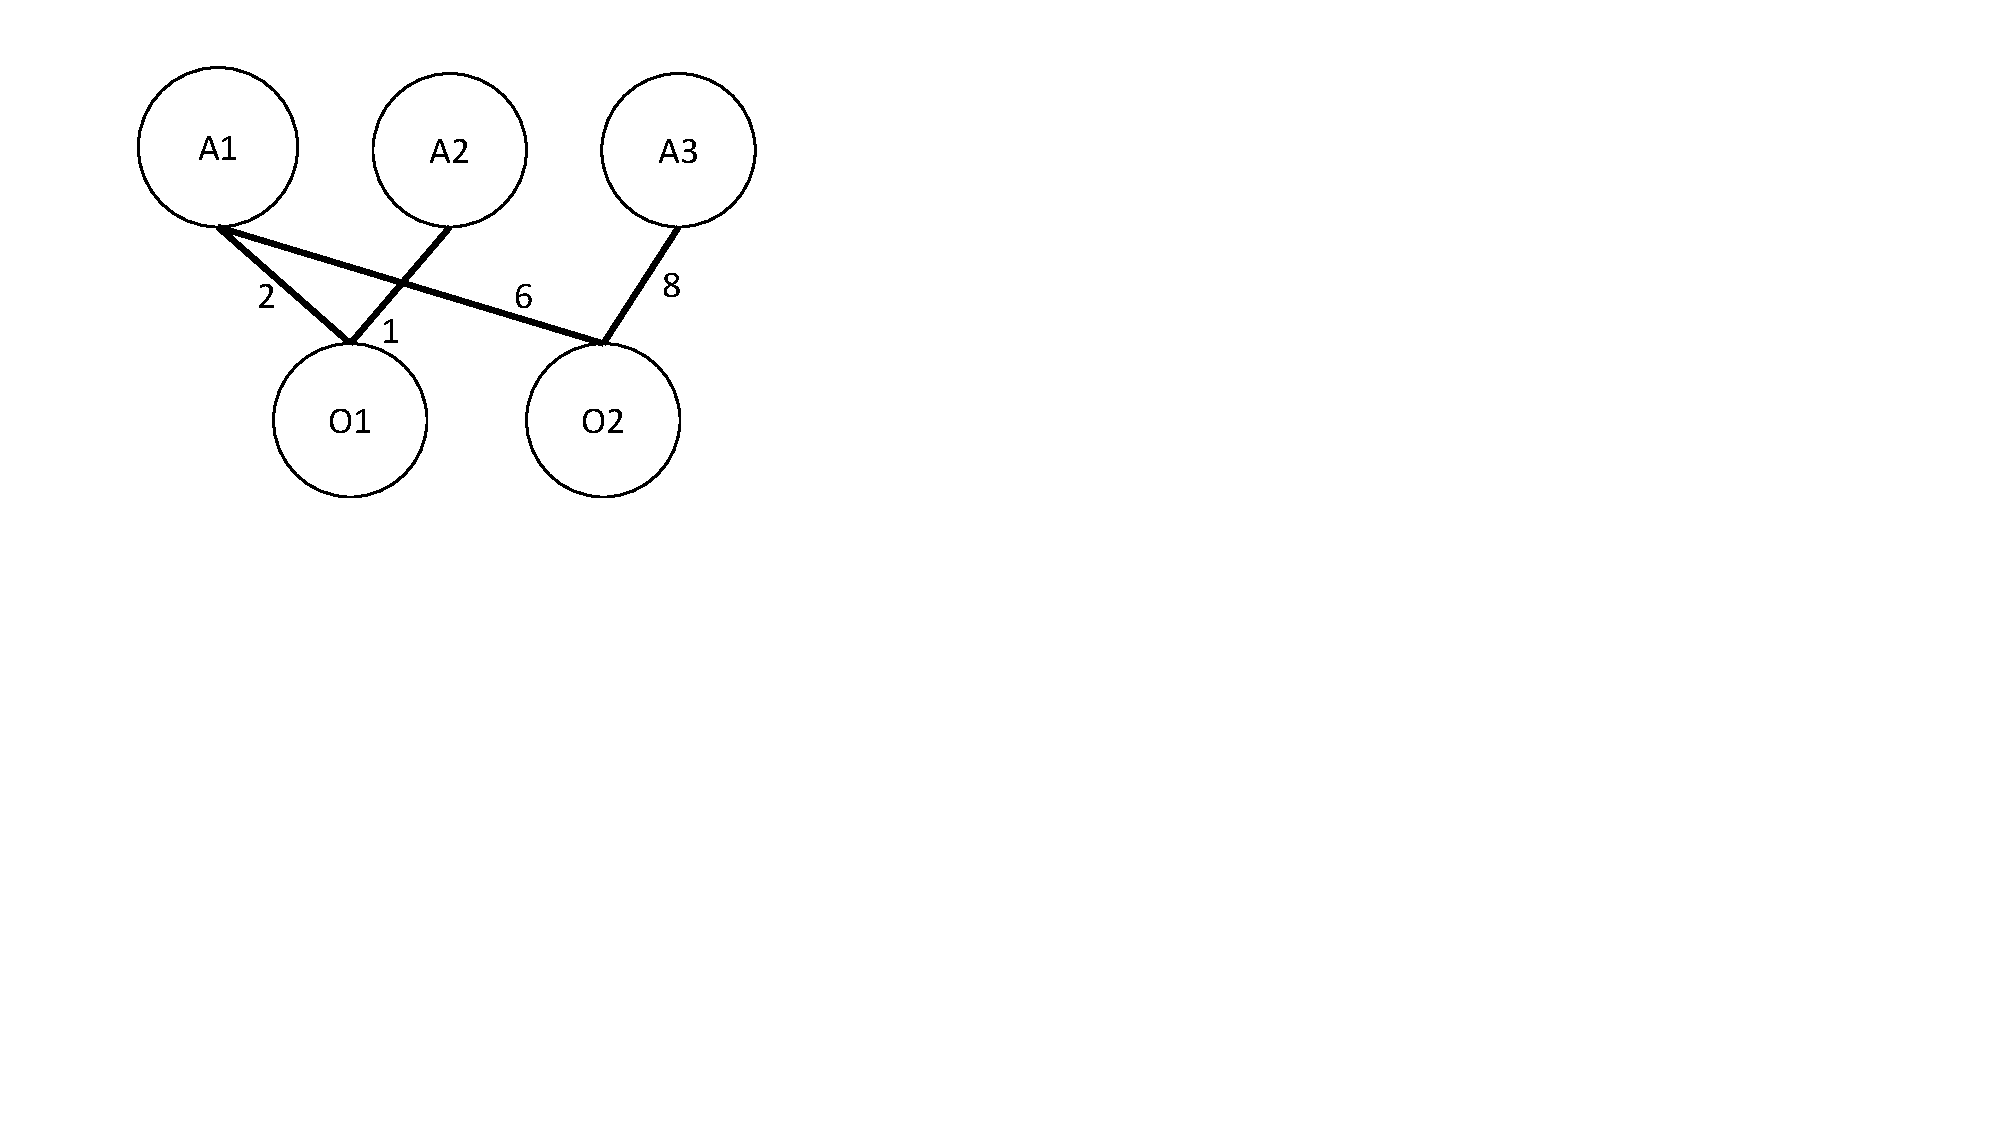
\includegraphics[width=10cm, trim={1.5cm 9.5cm 16.0cm 0cm}]{img/MatchCluster.pdf}
	\caption{Match Activity Cluster (A1-A3) and Object Cluster (O1-O2)}
	\label{fig:matchCluster}
\end{figure}


Speaking the first approach, each data object cluster is simply matched to the activity cluster that is connected by th edge with the highest weight. Further, merge object clusters that match the same activity cluster. Activity clusters that have not been matched to a data object cluster remain without accompanying data objects, i.e. not merge with another activity cluster to avoid the combination of two different bounded contexts. Whereas this approach is straight forward and easy to apply, it has drawbacks: The cluster matching from data object point of view does not consider the overall dependencies. Regarding Fig.\ref{fig:matchCluster}, the result would be \textit{(O1,A1),(O2,A3),A2}. Despite the fact that \textit{A1} accesses \textit{O2} six times, it is outweighed by the combination \textit{O2,A3}.  \\
The second approach is similar as each activity cluster is matched to the object cluster that is connected by th edge with the highest weight. Activity clusters that match the same object clusters are merged. Solely object clusters that remain unmatched in the end need to be matched with one of its connected activity clusters, as the data needs to be available somewhere. The best fit in regard to data accesses is the connected activity cluster node with the highest edge weight. In this case, the result obtained from Fig.\ref{fig:matchCluster} would be \textit{(A1,A3,O2),(A2,O1)}. Like the first approach, overall dependencies are not noticed. \\
In order to avoid this, i.e. to consider the dependencies holistically, the third approach uses the same clustering algorithm as proposed in Sec.\ref{sec:Solution:IdentifyCluster}. Thus, high cohesive activity and data object clusters are combined. In regard to the case study \textit{CoCoME}, this approach provided satisfactory results. However, the clustering method usually merges activity clusters which can result in a too coarse-grained final microservice decomposition recommendation. So far, none of the approaches consider to split data object or activity clusters. For that, a closer look to the actual activity-data-relationships has to be taken. \\
In the following, we present a conceptual solution to match the two types of clusters according to their profound relationships. Hence, a white box approach is proposed: First, the clustering as presented previously is applied to achieve a first decomposition. As mentioned before, this step combines high cohesive data object clusters and activity clusters. In the next step, each combined cluster is scrutinized more precisely. In the situation that a combined cluster consists only of one activity and one data object cluster, there is nothing to do. If two (or more) activity clusters are merged and reference one data object cluster, it is necessary to take a closer look at the actual data objects they reference. In case both activity clusters reference mostly the same set of data objects in that cluster, merging is useful as distributing the activities in different services causes inevitable cross-service communication. Splitting object clusters is reasonable if it becomes apparent that one part of the data objects are referenced mostly by one activity cluster and the other part by the other activity clusters. Consequently, the previously identified set of activity clusters and the data cluster is divided into smaller parts while preserving the internal cohesion between data and activities and while keeping the combined cluster small. \\
This solution is not yet mature and only presented conceptional. Neither a concise definition is provided nor has it been tested on several case studies. However, we believe in the potential of the solution and propose a more detailed case study in the area of cluster matching. Although we are aware that the third solution may produce too coarsely granular results, we chose this one,for now, to match the identified data object clusters and activity clusters. \\





\section{Extract Microservice Candidates}
\label{sec:Solution:ExtractMicroserviceCandidates}
So far, BPMN models were used to extract the control flow and the data flow from a system's business processes. Based on heuristics, we determined dependencies between the activities and between the data objects and visualized them as two graphs to identify clusters of dense relationships that are weakly connected to other clusters. In the previous section, we proposed different approaches to match the activity clusters and the object clusters in order to obtain combined cluster. Those clusters correspond to the microservice candidates: The activities describe the functionality that the microservice provides. The data object clusters describe the data object which the microservice has to administer. This includes the availability of interfaces to share data with other services if necessary.
Those combined clusters are good candidates to become a microservice, because:
\begin{itemize}
	\item Most of the data objects are accessed by activities within the service, which satisfies the low coupling criteria.
	\item Cohesive functionality is placed in the same service, which satisfies the high cohesion criteria.
	\item The approach reduces inter-service communication to a minimum, which enhances the performance.
\end{itemize}

This step finalizes the microservice identification approach. In the following, it is applied to the case study CoCoME (cf. Chapter \ref{ch:CoCoME}). 











\chapter{Application of the Approach}
\label{ch:SolutionApplication}
This chapter applies the previously presented approach to identify microservices from the business point of view, using clustering on control flow and data flow. It is applied to CoCoME, whose system specifications are defined in chapter \ref{ch:CoCoME}. Speaking of the order, this chapter follows the process overview illustrated by Fig.\ref{fig:thesisProcess}.

\section{Use Cases as BPMN Models}
CoCoME's system specifications are given in terms of use cases. A short overview is available in chapter \ref{ch:CoCoME}, whereas a more detailed version can be found in the \textit{Technical Report} \cite{CoCoMETechnical}. We decide to omit  \textit{UC 8 - Product Exchange} as independent BPMN model, because both reference sets either did not take it into consideration or implemented it differently. However, it was added as extension to \textit{UC 1} as single activity named \textit{Product Exchange}. In the same way, \textit{UC 2 - Manage Express Checkout} is added to \textit{UC 1} as single activity named \textit{Manage Express Checkout}. \textit{UC 2} extends \textit{UC 1} and therefore, has to be associated with \textit{UC 1} anyway.  Fig.\ref{fig:UC1} illustrates \textit{UC 1,2} and \textit{8} as BPMN model. The remaining BPMN models are available in the appendix (cf. \ref{sec:appendix:BPMN Models}). For the sake of clarity, the models are not yet joined as described in section \ref{sec:PrepApproach:TransformUCtoBPMN}. Apart from Fig.\ref{fig:UC1}, each use case is illustrated as single BPMN process. However, the BPMN models that represent \textit{UC 3} and \textit{UC 4} as well as \textit{UC 4} and \textit{UC 1} need to be joined, as preconditions and postconditions are equal. 

%TODO Connection 


%"l, b, r, t"
\begin{figure}[h!]
	\centering
	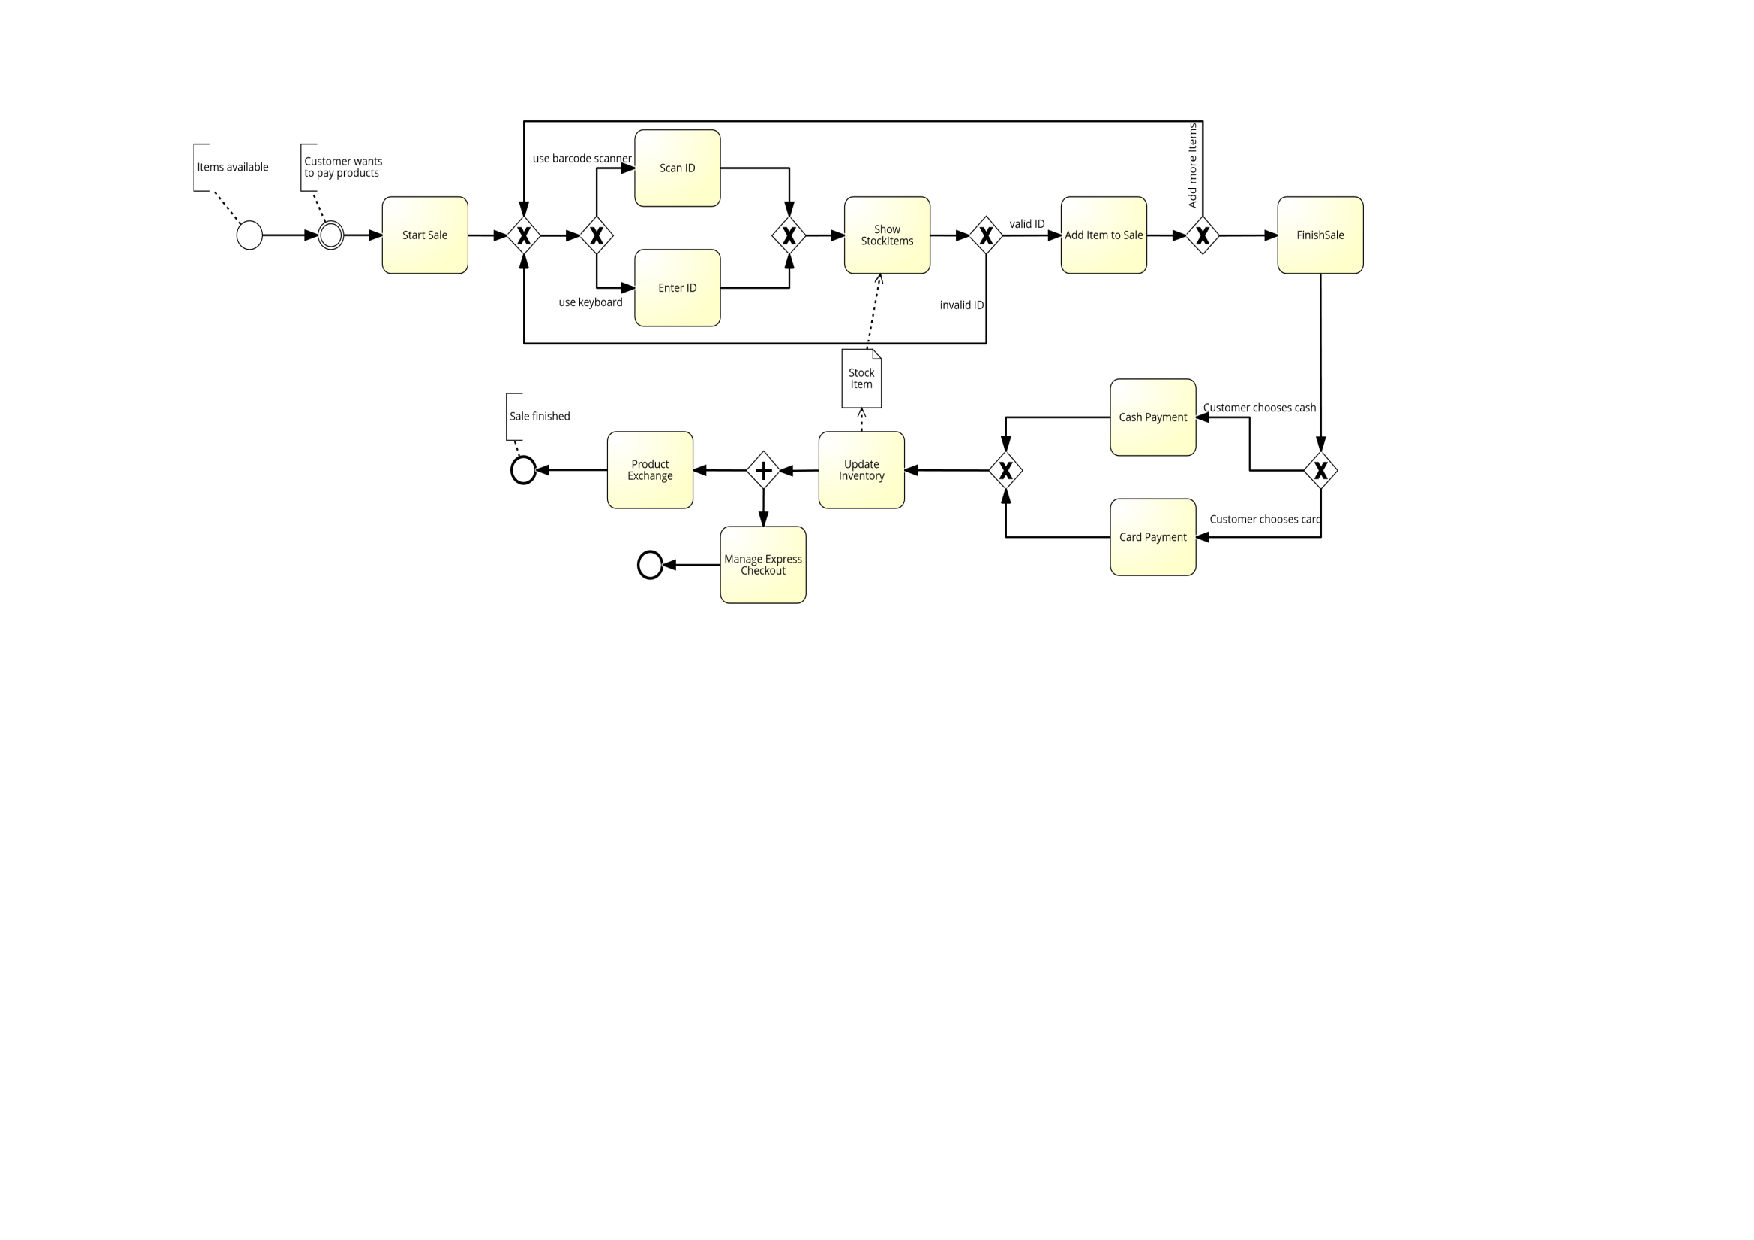
\includegraphics[width=\textwidth, trim={4cm 10.5cm 8cm 2cm}]{img/UC1.pdf}
	\caption{UC1-Process Sale (with UC2 and UC8)}
	\label{fig:UC1}
\end{figure}




\section{Extracted Control Flow}

In this step, the control flow is extracted from the BPMN models. Sec. \ref{sec:Solution:ExtractControlFlow} provides the detailed extraction process, but in a word, everything but the control flow elements are deleted. Fig.\ref{fig:UC3Control} presents the control flow for \textit{UC 3}. The remaining control flow diagrams are available in the appendix (cf. \ref{sec:appendix:ControlFlow}).  

%"l, b, r, t"
\begin{figure}[h!]
	\centering
	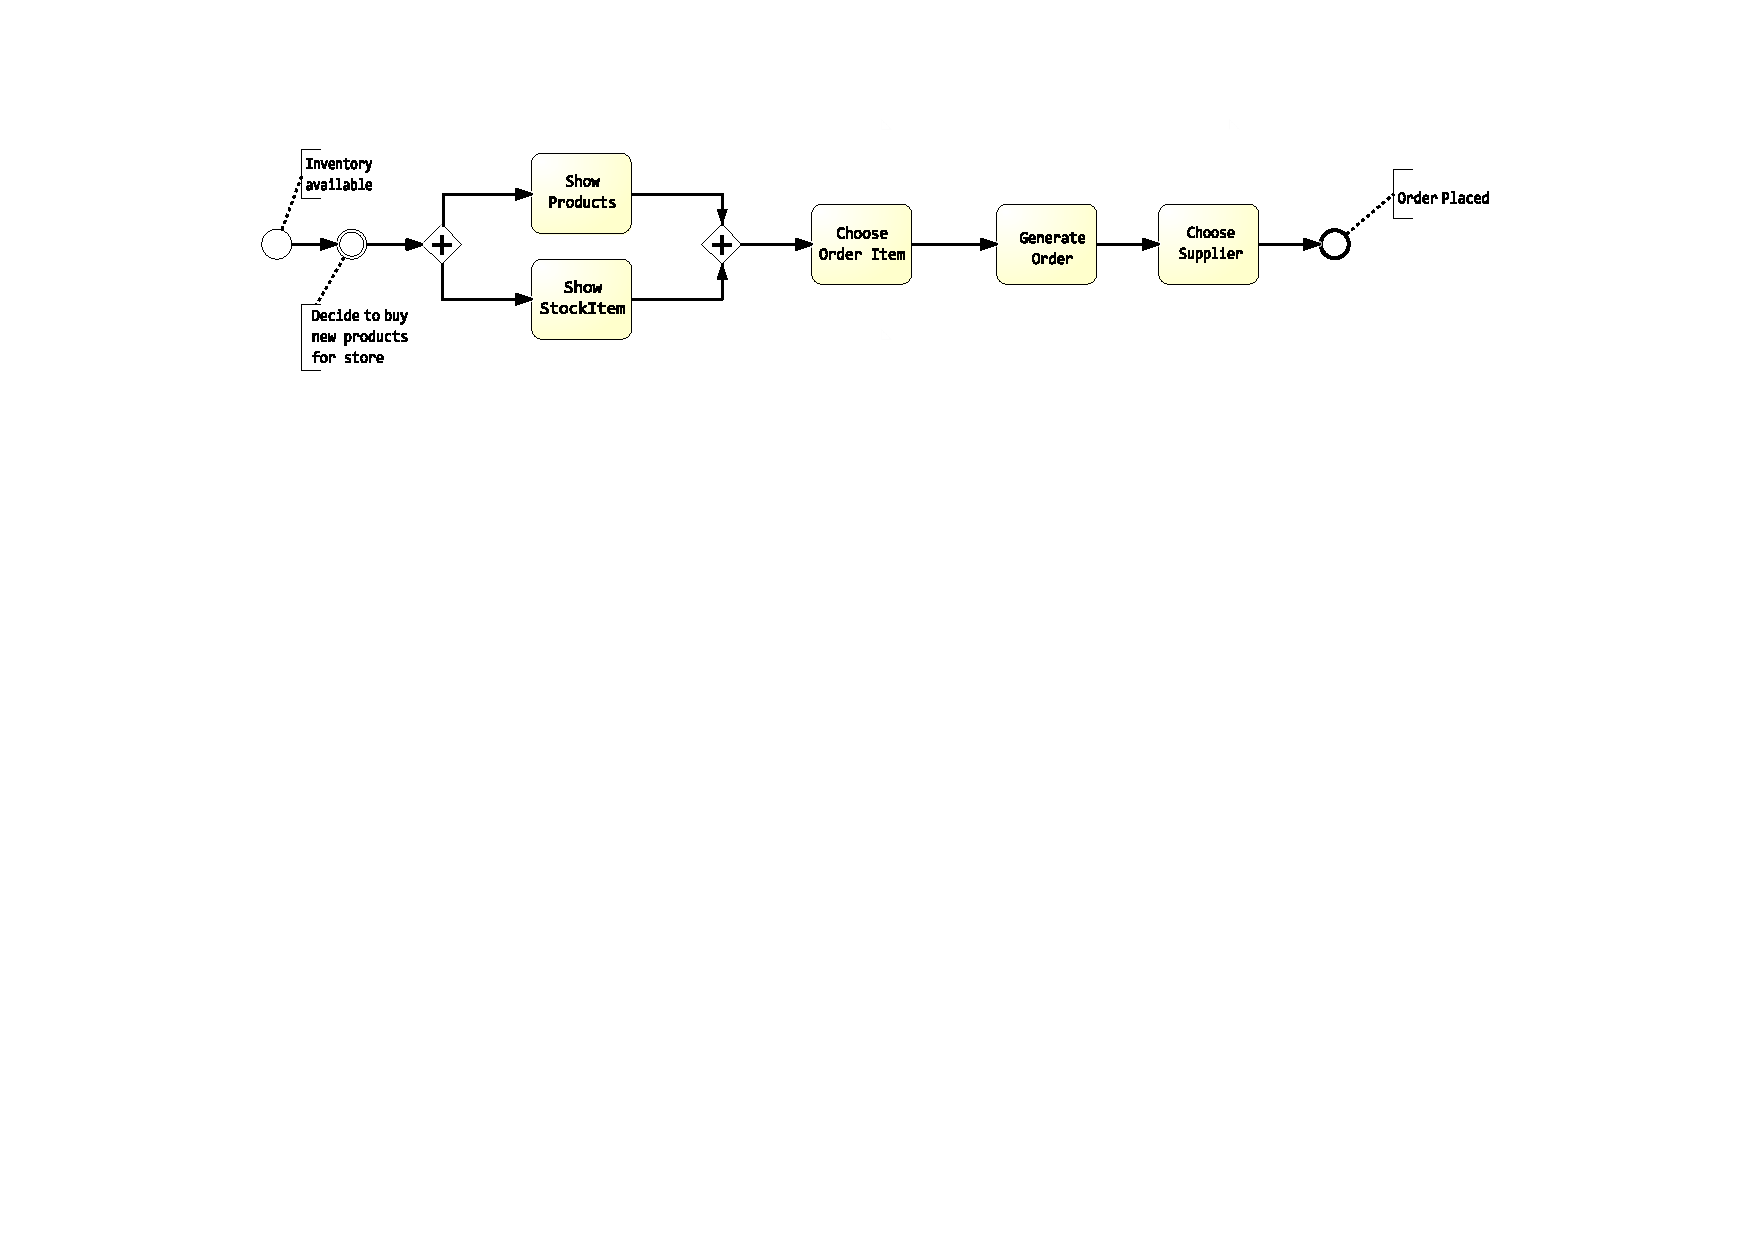
\includegraphics[width=\textwidth, trim={5cm 14cm 6cm 2cm}]{img/UC3Control.pdf}
	\caption{Control Flow UC3 - Order Products}
	\label{fig:UC3Control}
\end{figure}

\section{Extracted Data Flow}

Like the previous step, the data flow is extracted from the BPMN models as described in Sec.\ref{sec:Solution:ExtractDataFlow}. Fig.\ref{fig:UC3Control} presents the data flow for \textit{UC 3}. The remaining data flow diagrams are available in the appendix (cf. \ref{sec:appendix:DataFlow}).

%"l, b, r, t"
\begin{figure}[h!]
	\centering
	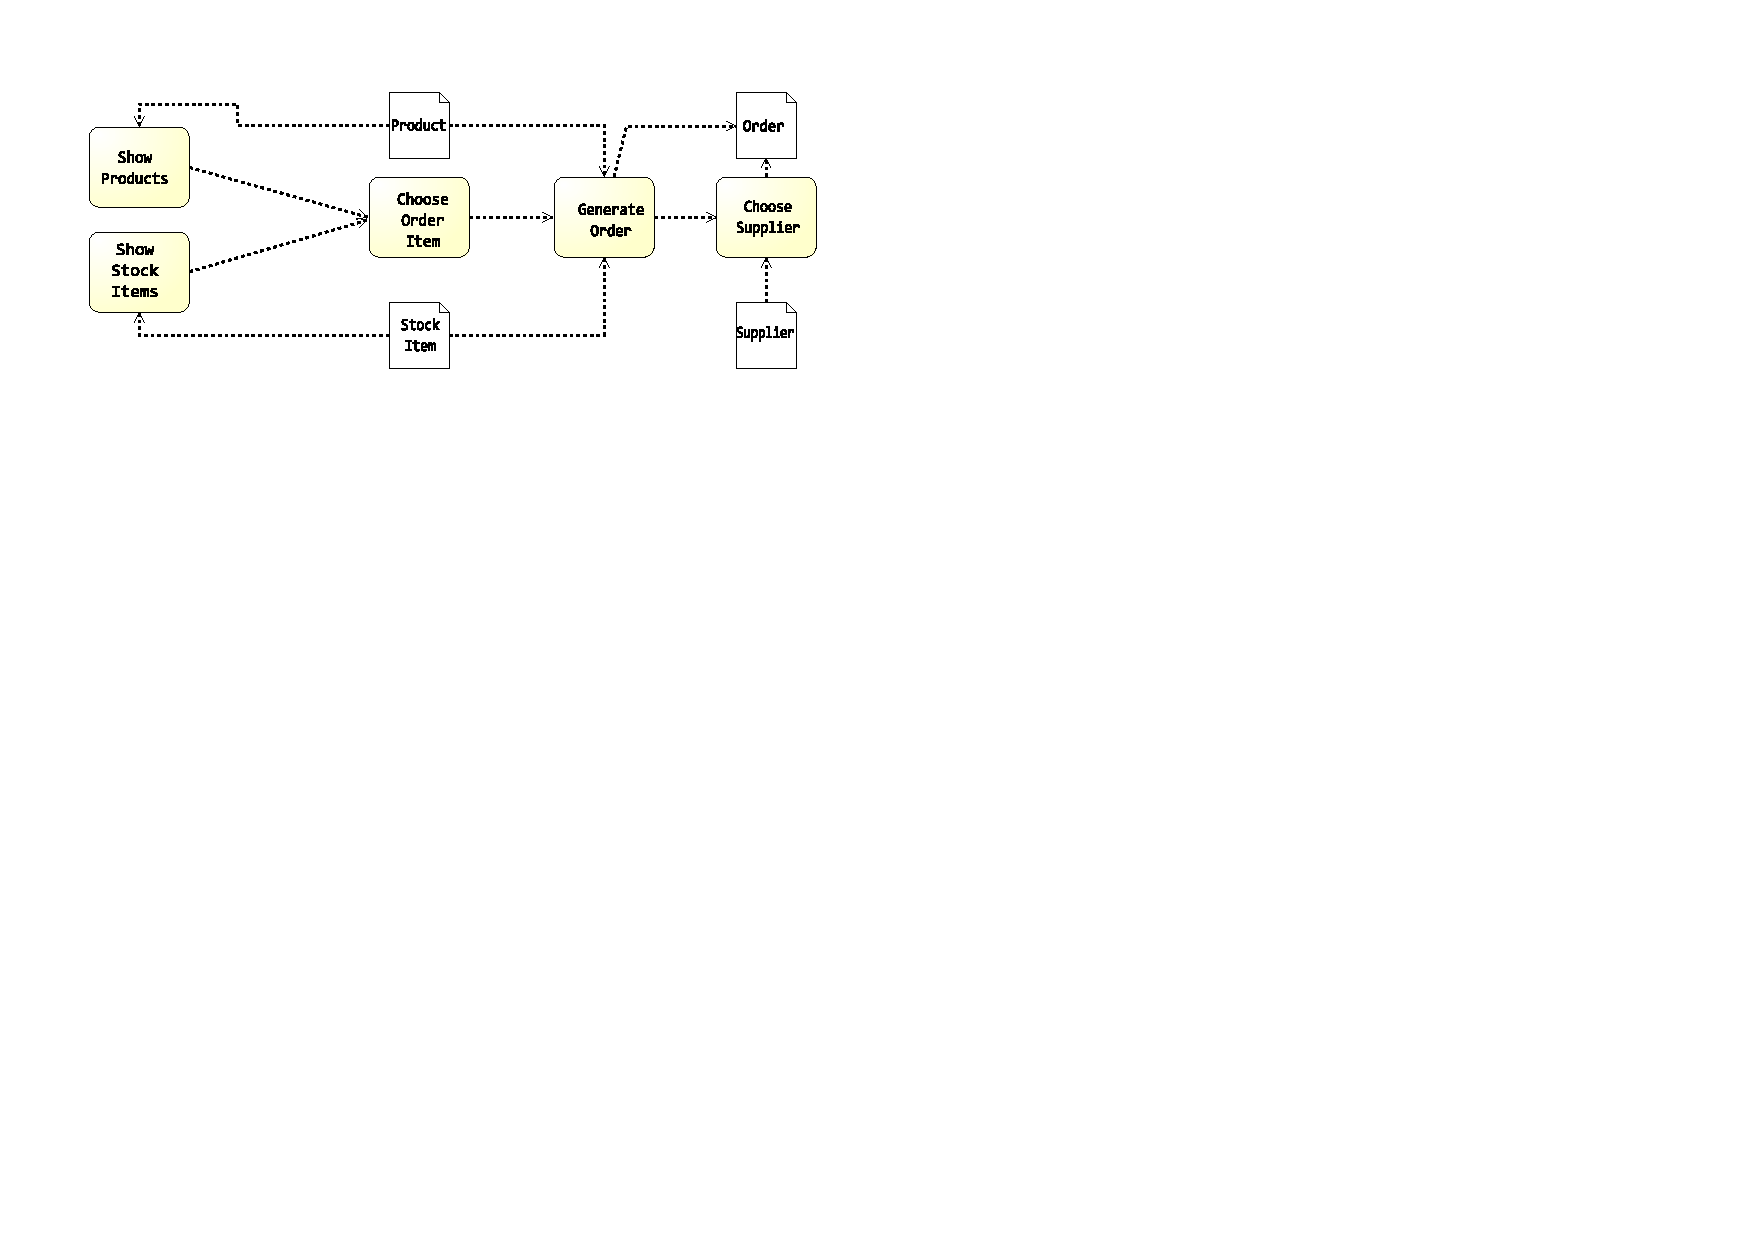
\includegraphics[width=8cm, trim={5cm 14cm 17cm 0cm}]{img/UC3DFD.pdf}
	\caption{Control Flow UC3 - Order Products}
	\label{fig:UC3DFD}
\end{figure}

\section{Control Flow Graph}
Fig.\ref{fig:CoCoMEControlFlowGraph} illustrates the control flow graph of CoCoME which is derived from the control flow diagrams. 

%"l, b, r, t"
\begin{figure}[h!]
	\centering
	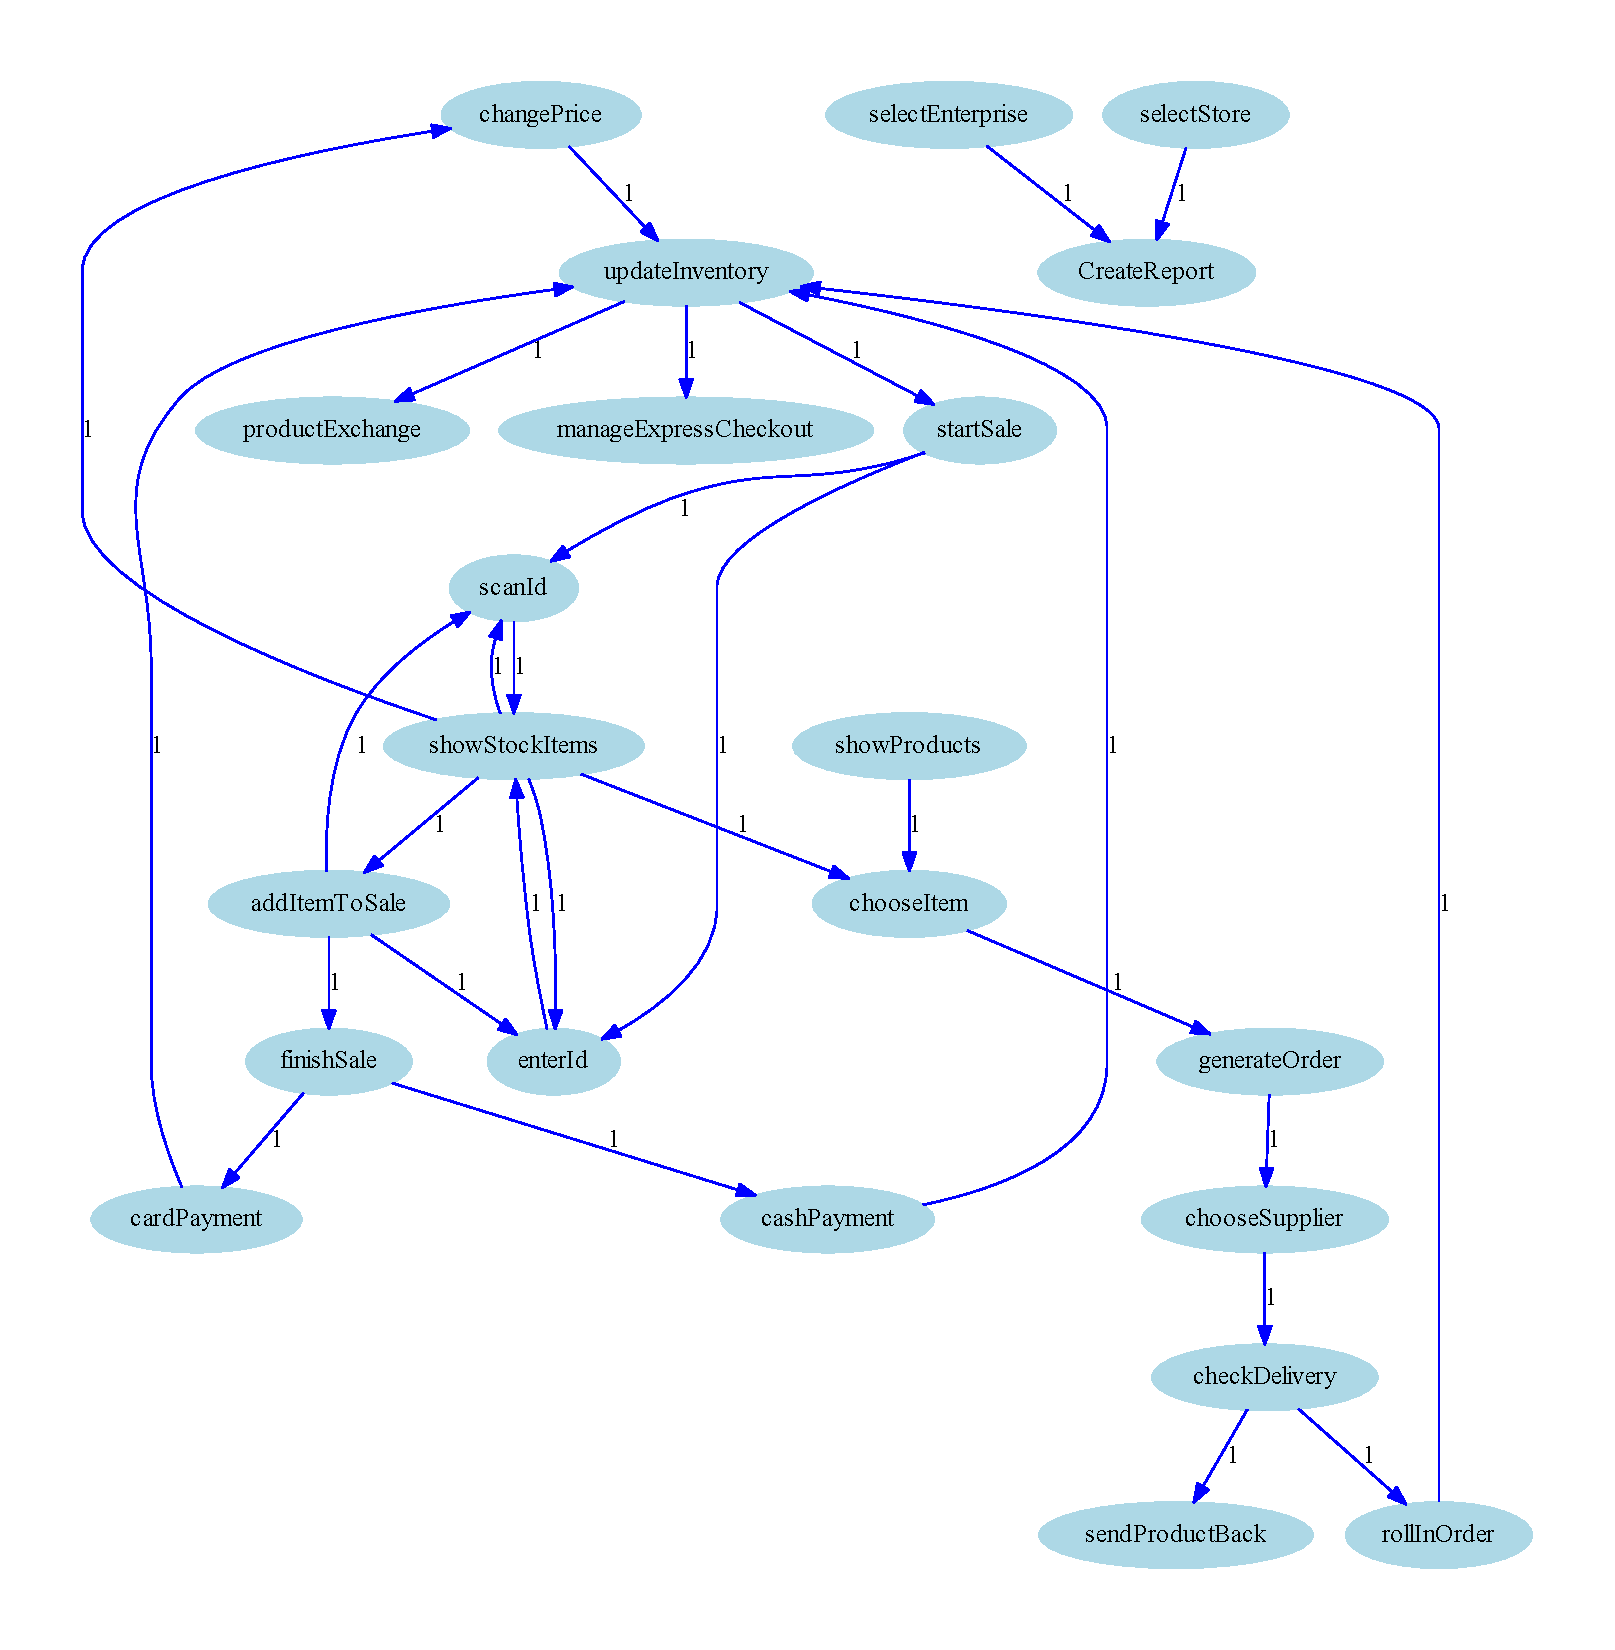
\includegraphics[width=\textwidth, trim={2cm 0cm 2cm 0cm}]{img/CoCoMEControlFlowGraph.pdf}
	\caption{Control Flow Information as Graph CoCoME}
	\label{fig:CoCoMEControlFlowGraph}
\end{figure}


\section{Data Flow Graph}

Fig.\ref{fig:CoCoMEDataFlowGraph} illustrates the data flow graph of CoCoME which is derived from the data flow diagrams. When identifying the data flow dependencies, it is necessary to choose a value for the parameter \textit{n}, that describes the maximum distance between a pair of activities that consume and produce a data object. We use \textit{n=1}, as it produces the most appropriate results compared to the final microservice decomposition. 

%"l, b, r, t"
\begin{figure}[h!]
	\centering
	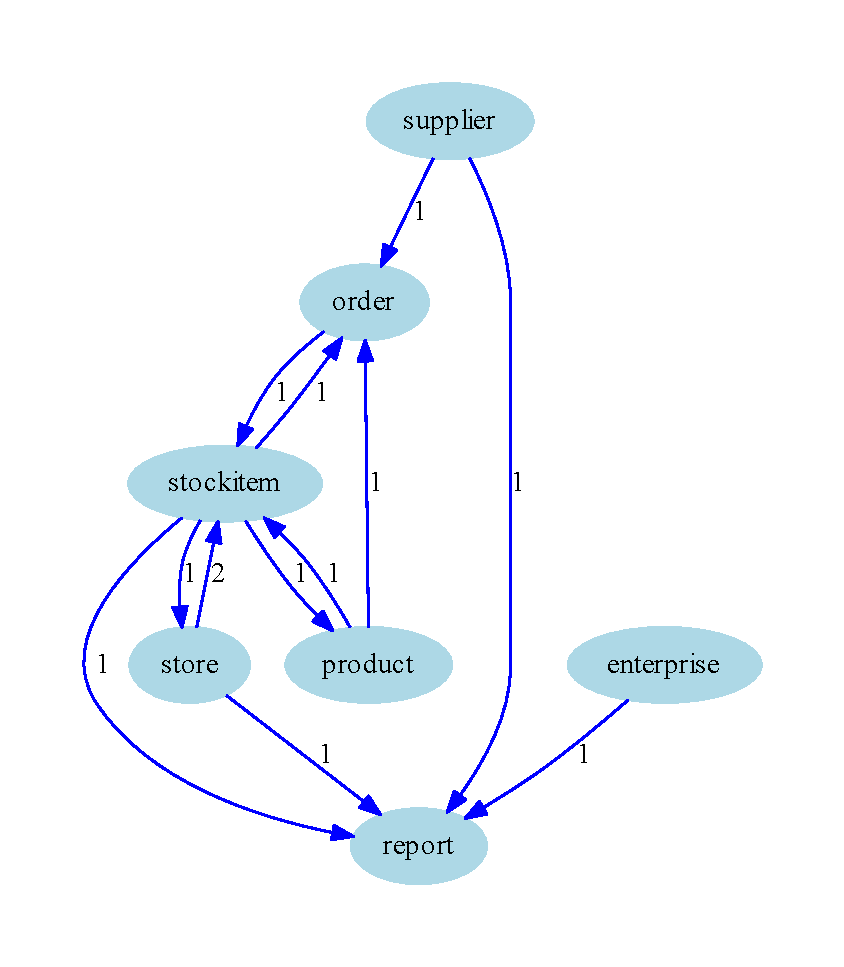
\includegraphics[width=10cm, trim={1cm 0cm 2cm 0cm}]{img/CoCoMEDataFlowGraph.pdf}
	\caption{Data Flow Information as Graph CoCoME}
	\label{fig:CoCoMEDataFlowGraph}
\end{figure}

\pagebreak

\section{Activity Clusters}
Fig.\ref{fig:CoCoMEActivityCluster} shows the activity clusters that are identified using the clustering algorithm described in Sec.\ref{sec:Solution:IdentifyCluster}. The naming is inspired by the actual implementation of CoCoME \cite{NikoCoCoMEImpl}.

%"l, b, r, t"
\begin{figure}[h!]
	\centering
	\begin{sideways}
		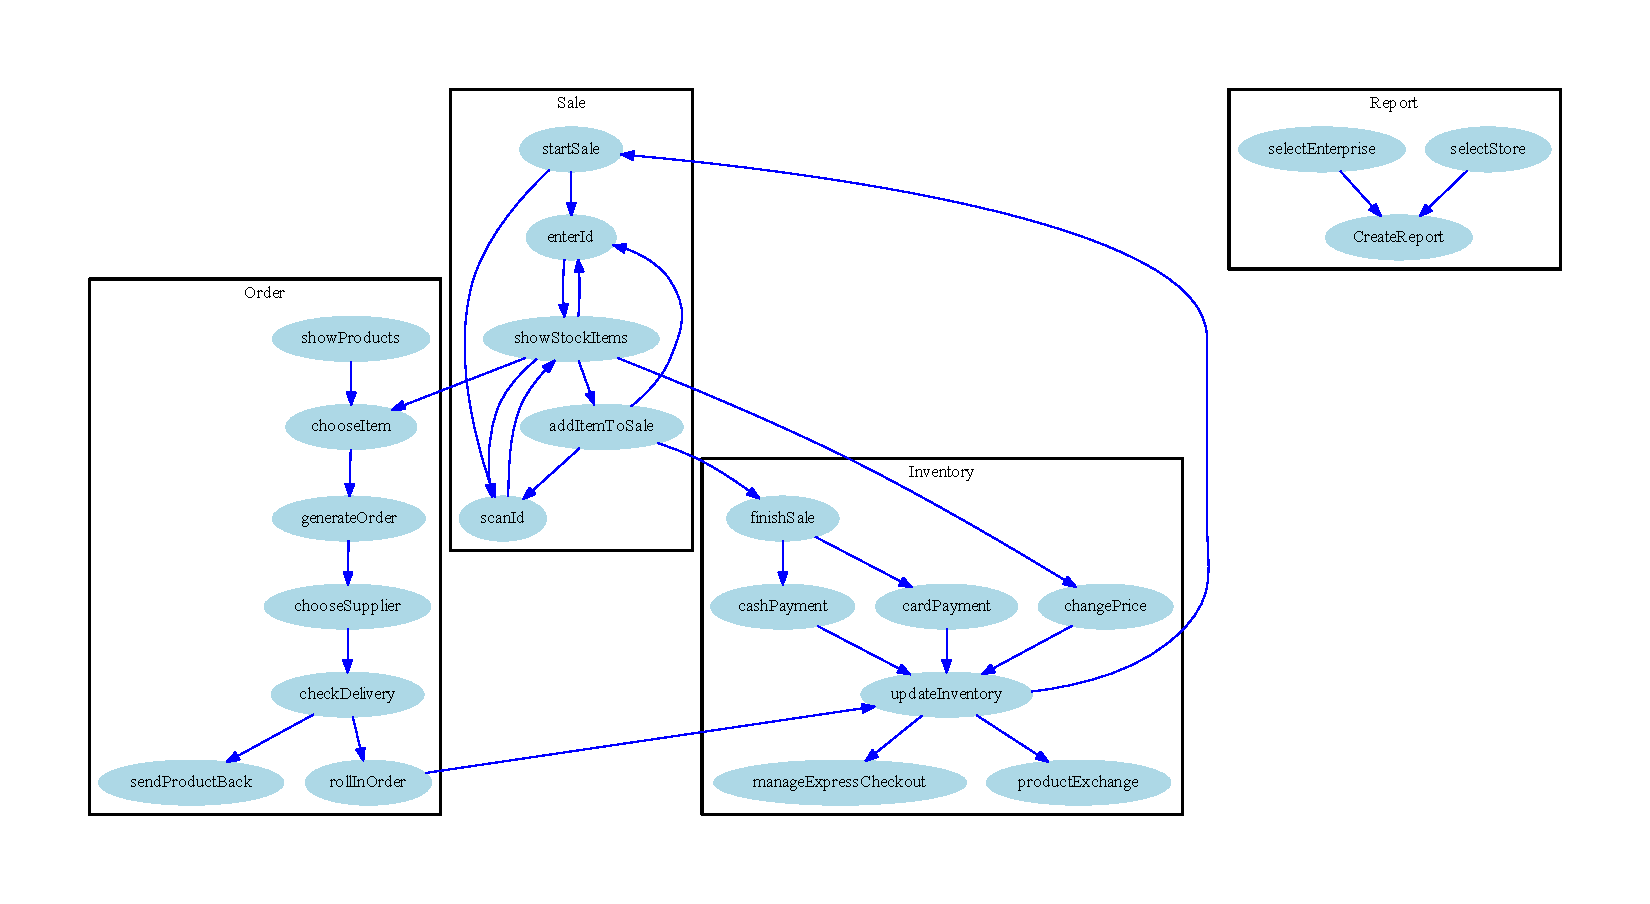
\includegraphics[width=19.0cm, trim={1.5cm 0cm 1.8cm 0cm}]{img/CoCoMEActivityCluster.pdf}
	\end{sideways}
	
	\caption{Clustering on CoCoME's Activities}
	\label{fig:CoCoMEActivityCluster}
\end{figure}



\section{Data Object Clusters}
Fig.\ref{fig:CoCoMEActivityCluster} shows the data object clusters that are identified using the clustering algorithm described in Sec.\ref{sec:Solution:IdentifyCluster}.
%"l, b, r, t"
\begin{figure}[h!]
	\centering
	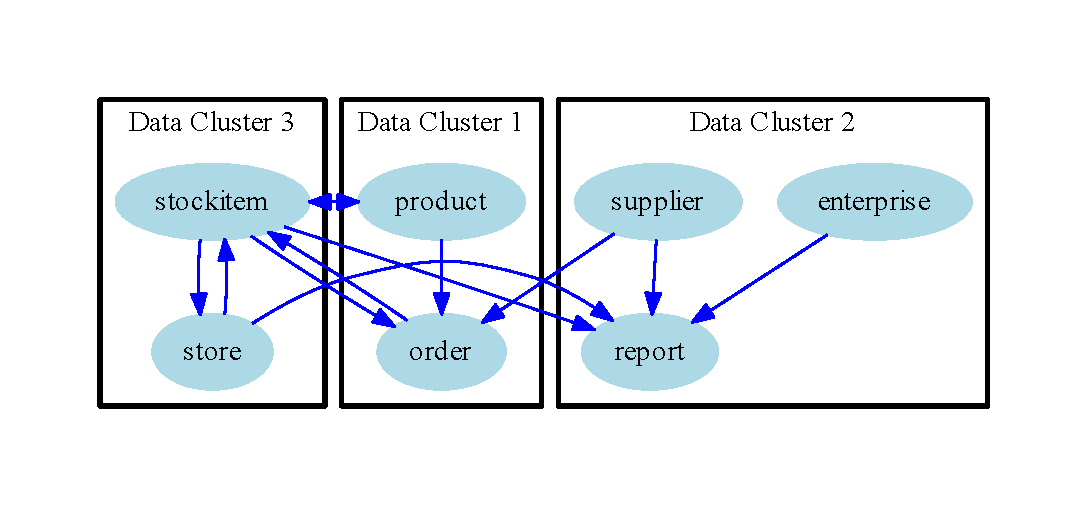
\includegraphics[width=12cm, trim={2cm 0cm 2cm 0cm}]{img/CoCoMEDataClusterWith1.pdf}
	\caption{Clustering on CoCoME's Data Objects}
	\label{fig:CoCoMEDataCluster}
\end{figure}

\section{Match Clusters}
In the following, the data object clusters and the activity clusters are matched. Section \ref{sec:Solution:MatchCluster} provides several solutions, including one that is only given conceptional and still raises too many uncertainties. Consequently, the matching is done by applying the black box clustering approach. Hence, the data access dependencies between data object and activity cluster need to be elaborated first. \\




%"l, b, r, t"
\begin{figure}[h!]
	\centering
	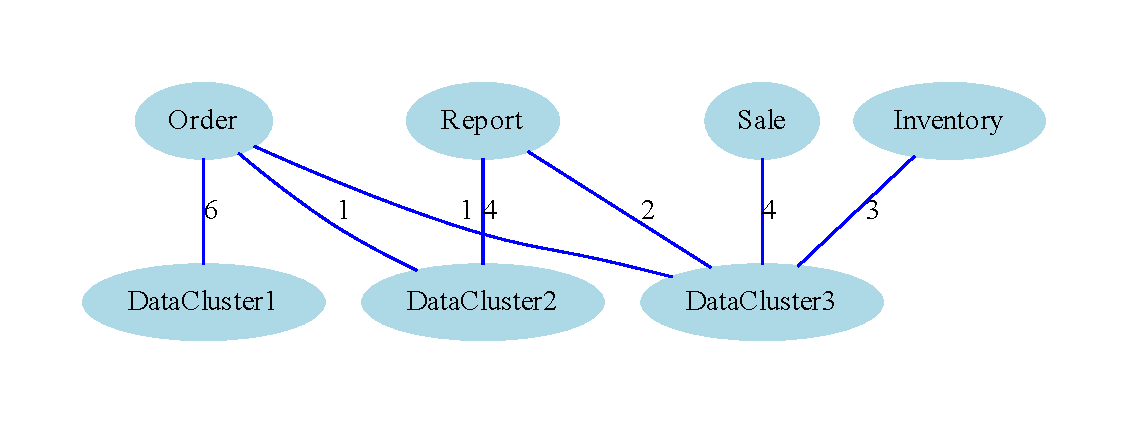
\includegraphics[width=12cm, trim={2cm 1cm 2cm 0cm}]{img/MatchClusterGraph.pdf}
	\caption{Data Access Dependencies between Data Object Clusters and Activity Cluster of CoCoME}
	\label{fig:CoCoMEClusterGraph}
\end{figure}

 Fig.\ref{fig:CoCoMEClusterGraph} illustrates the data access dependencies between the four activity clusters \textit{Order, Report, Sale} and  \textit{Inventory} and the \textit{DataClusters 1-3}. The weights correspond to the amount of read and write accesses between activities and data objects within the corresponding clusters.  \\
 Finally, the clustering method introduced in Sec.\ref{sec:Solution:IdentifyCluster} identifies cohesive clusters of activity cluster nodes and data object cluster nodes.



%"l, b, r, t"
\begin{figure}[h!]
	\centering
	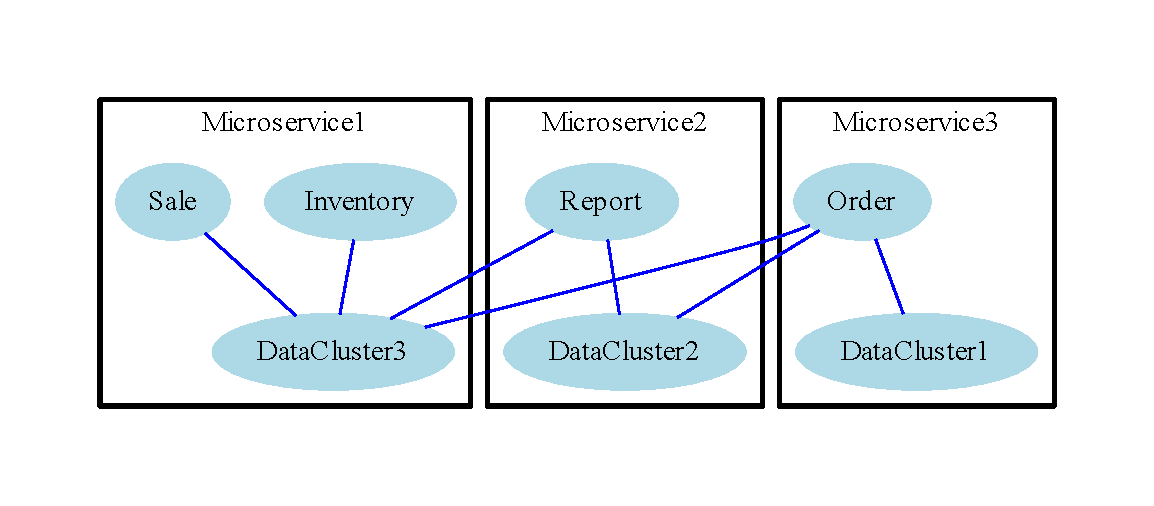
\includegraphics[width=12cm, trim={2cm 1cm 2cm 0cm}]{img/MatchClusterClustering.pdf}
	\caption{Proposed Microservice Decomposition of CoCoME}
	\label{fig:CoCoMEClusterMatching}
\end{figure}



\section{Extract Microservice Candidates}
In the previous step, cohesive clusters of activity cluster nodes and data object cluster nodes are identified. Each of the combined clusters correspond to a microservice candidate. Fig.\ref{fig:CoCoMEClusterMatching} illustrates the  microservices that are identified. To compare the outcome with other results, it is necessary to elaborate the functionality that is provided by each microservice as well as the accompanying data objects. To be able to compare it with the reference sets, the functionalities must be renamed and abstracted. For example, \textit{startSale} and \textit{finishSale} become \textit{Handle sale} or \textit{enterId} and \textit{showStockItems} become \textit{Identify stock items}. \\



\begin{multicols}{3}
	\textbf{Microservice 1}
	\begin{flushleft}
	\begin{itemize}[noitemsep]
	\item Handle sale
	\item Handle payment
	\item Manage express checkout
	\item Exchange products
	\item Identify stock items
	\item Handle inventory
	\item Change price
	\item \textbf{Data objects}: stockItem, store
	\end{itemize}
	\end{flushleft}


	\vfill
	\columnbreak
	\textbf{Microservice 2}
	\begin{flushleft}
	\begin{itemize}[noitemsep]
	\item Create delivery report
	\item Create stock report
	\item \textbf{Data Objects}: supplier, report, enterprise
    \item[]
    \item[]
    \item[]
    \item[]
    \item[]
    \item[]
	\end{itemize}
	\end{flushleft}
	
	
	\vfill
	\columnbreak
	\textbf{Microservice 3}
	\begin{flushleft}
	\begin{itemize}[noitemsep]
		\item Show products
		\item Create orders
		\item Handle deliveries
		\item Show suppliers
		\item \textbf{Data Objects}: product, order
	\end{itemize}
\end{flushleft}
\end{multicols}












\chapter{Evaluation}
\label{ch:Evalutation}
In the introduction chapter, the \textit{Research Questions} are presented. The third question relates to the elaborated approach and its evaluation. 


\vspace{0.5cm}
\par
\begingroup
\leftskip=1cm
\rightskip=1cm

\noindent
\textbf{RQ1.3: What is the accuracy of the approach? }

\endgroup
\vspace{0.5cm}

\noindent
To answer this question efficiently, a \textit{Goal Quality Metrics Plan } (GQM) is to be created that specifies the key aspects of the evaluation. 
Chapter \ref{ch:SolutionApplication} applies the identification approach to the running example. As a result, a set of microservices is identified where each microservice provides some functionalities and administers data objects.\\
In order to evaluate this approach, we compare those results to two reference sets. In doing so, not only is it checked whether the right services have been found, but also whether the functionality and the data objects have been divided up correctly. During the evaluation, those aspects are examined independently. Functionality in this sense is a service offered by a microservice that is comprehensible and understood by non-technical stakeholders. \\
The rest of the chapter is structured as follows: First, the evaluation goals and metrics are introduced. Second, the design of the evaluation is demonstrated, including the presentation of two reference sets which are used to compare the output of the approach, when applied to the running example. Third, the evaluation results are presented. Second to last, the evaluation results are discussed. Eventually, the threats to the validity are outlined.


\section{Evaluation Goals and Metrics}

\subsection{Evaluation Goals}
\label{sec:Evaluation:GQM}
Basili \textit{et al.} originally proposed the \textit{GQM Plan} (Goal Quality and Metrics) as a paradigm in software engineering to create specific quality models \cite{BasiliGQM}. \\
The main purpose of the \textit{GQM Plan} is to identify the right metrics to assess the quality of an object in a particular environment. This should prevent the gathering of unnecessary metrics and measurements and consequently reduce the expenditure of work. \\
The \textit{GQM Plan} is a Top-Down approach and is divided in three fundamental steps that precede the measurement and evaluation of results. First, the goal of the evaluation is defined on a conceptual level. Second, questions are delineated to achieve the specific goal. Finally, to answer the questions in a measurable way, metrics have to be defined that are associated with the questions. \\
In the following, the \textit{GQM Plan} for the consecutive evaluation is detailed out:

\begin{itemize}
	\item \textbf{G1:} Determination of the accuracy of the approach to demonstrate that it is capable to identify adequate microservice candidates.
	\item \textbf{G1.Q1:} What is the \textit{Precision and Recall} of the identified microservices compared to the reference sets?
	\item \textbf{G1.Q1.M1:} Measure \textit{Precision and Recall } of the identified microservice.
	\item \textbf{G1.Q2:} What is the \textit{Precision and Recall} regarding the functionality of the identified microservices compared to the reference sets?
	\item \textbf{G1.Q2.M1:}  Measure \textit{Precision and Recall} of the identified functionalities.
	\item \textbf{G1.Q3:} What is the \textit{Precision and Recall} regarding data objects each microservice administers compared to the reference sets?
	\item \textbf{G1.Q3.M1:}  Measure \textit{Precision and Recall} of the identified data objects.

\end{itemize}




\subsection{Evaluation Metrics}
\label{sec:Evaluation:Metrics}

Using metrics is mandatory to measure the quality of the elaborated approach. In this case, it is required to choose a metric that is capable of classifying a set of instances regarding their relevance.
In regard to the following evaluation, those instances are either microservices, functionalities offered by microservices or data objects administered by microservices. Two reference sets are available as further depicted in Sec.\ref{sec:Evaluation:ReferenceSets}. \\
A metric that is capable to measure the relevance of a set of instances compared to a reference set is \textit{Precision and Recall}. Subsequently, the proposed metric is briefly presented.

\subsection{Precision and Recall}
\label{sec:Evaluation:Metrics:sPrecRecall}
\textit{Precision and Recall} is a classification metric that measures the relevance of retrievable items with respect to a reference set \cite{PrecisionRecall}. Commonly, two distinctions for items in the reference set are made: First, Retrieved or not Retrieved. More precisely, an item is retrieved if it is part of the selected items and vice versa. Secondly, Relevant or Not Relevant. As a result, all retrievable items belong to exactly one of four cells in the following matrix:


\begin{table}[!h]
	\centering
	\begin{tabular}{|l||l|l|l|}
		\hline
		& Relevant & Not Relevant & Sum \\ \hline
		Retrieved     &     $N_{ret\cap rel}$     &     $N_{ret\cap \overline{rel}}$            &     $N_{ret}$  \\ \hline
		Not Retrieved &      $N_{\overline{ret}\cap rel}$      &      $N_{\overline{ret}\cap \overline{rel}}$          &    $N_{\overline{ret}}$   \\\hline
		Sum           &         $N_{rel}$   &      $N_{\overline{rel}}$          &    $N_{total}$   \\ \hline
		
	\end{tabular}
\caption{Retrieval Matrix, Source: \cite{PrecisionRecall}}
    \label{tab:PrecRecall}
    
\end{table}

\pagebreak

\noindent
\textbf{Recall} describes the completeness of the retrieval. In other words, how many relevant items are selected in regard to all possible relevant items.

\begin{centering}
	\vspace{1cm}
	
	$Recall=\dfrac{N_{ret\cap rel}}{ N_{rel} }  $
	
	\vspace{1cm}
\end{centering} 

\noindent
\textbf{Precision} illustrates the purity of the retrieval because it puts into proportion the number of retrieved relevant items and the number of all retrieved items.

\begin{centering}
	\vspace{1cm}
	
	$Precision=\dfrac{N_{ret\cap rel}}{ N_{ret} }  $
	
	\vspace{1cm}
\end{centering} 

 
\noindent
In both cases, the values range from zero to one, where a higher value represents a more satisfying value in terms of completeness and purity of the retrieval.
It is important to notice that $N_{\overline{ret}}$ and $N_{\overline{rel}}$ are not part of the formulas. With that in mind, it is possible to apply \textit{Precision and Recall} to the prevalent evaluation scenario. With respect to Table \ref{tab:PrecRecall}, the reference set used forms the relevant items, or $N_{rel}$. Accordingly, $N_{ret}$ constitutes the retrieved items which are either the actual microservices, the functionality provided by the microservices or the data objects administered by the microservices.
The remaining parts which are the non-relevant and non-retrieved items ($N_{\overline{ret}\cap \overline{rel}}$) are unimportant. The following list draws the analogy between Table \ref{tab:PrecRecall} and the predominant evaluation scenario:
\begin{itemize}
	\item \textbf{True Positives:}  $N_{ret\cap rel}$  
	
	\begin{itemize}
		\item Identified microservices that have a similar partner in the reference set \textbf{OR}
		\item Identified functionality that is assigned to the appropriate microservice \textbf{OR}
		\item Identified data objects that are assigned to the appropriate microservice
	\end{itemize}
	
	
	\item  \textbf{False Positives:}  $N_{ret\cap \overline{rel}}$ 
	\begin{itemize}
		\item Identified microservices that do not have a similar partner in the reference set \textbf{OR}
		\item Identified functionality, that is assigned to the wrong microservice  \textbf{OR}
		\item Identified data objects, that are assigned to the wrong microservice
	\end{itemize}
	
	\item \textbf{False Negatives}:  $N_{\overline{ret}\cap rel}$ 
		\begin{itemize}
		\item Microservices in the reference set that are not discovered by the proposed approach  \textbf{OR}
		\item Functionality in the reference microservices which is not discovered and allocated by the proposed approach  \textbf{OR}
		\item Data objects in the reference microservices which are not discovered and allocated by the proposed approach
	\end{itemize}
	
	\item \textbf{True Negatives}\footnote{Note, that this amount consists of all imaginable microservices and is therefore an infinite set. As it is not used to calculate either of the metrics, it is negligible. }: $N_{\overline{ret}\cap \overline{rel}}$
	 	\begin{itemize}
	 	\item  Microservices that are neither discovered by the approach, nor part of the reference set   \textbf{OR}
	 	\item Functionality that is neither distributed into a microservice, nor part of any microservice of the reference set  \textbf{OR}
	 	\item Data objects that are neither distributed into a microservice, nor part of any microservice of the reference set
	 \end{itemize}
	
	
	
\end{itemize}



\begin{figure}[!h]
	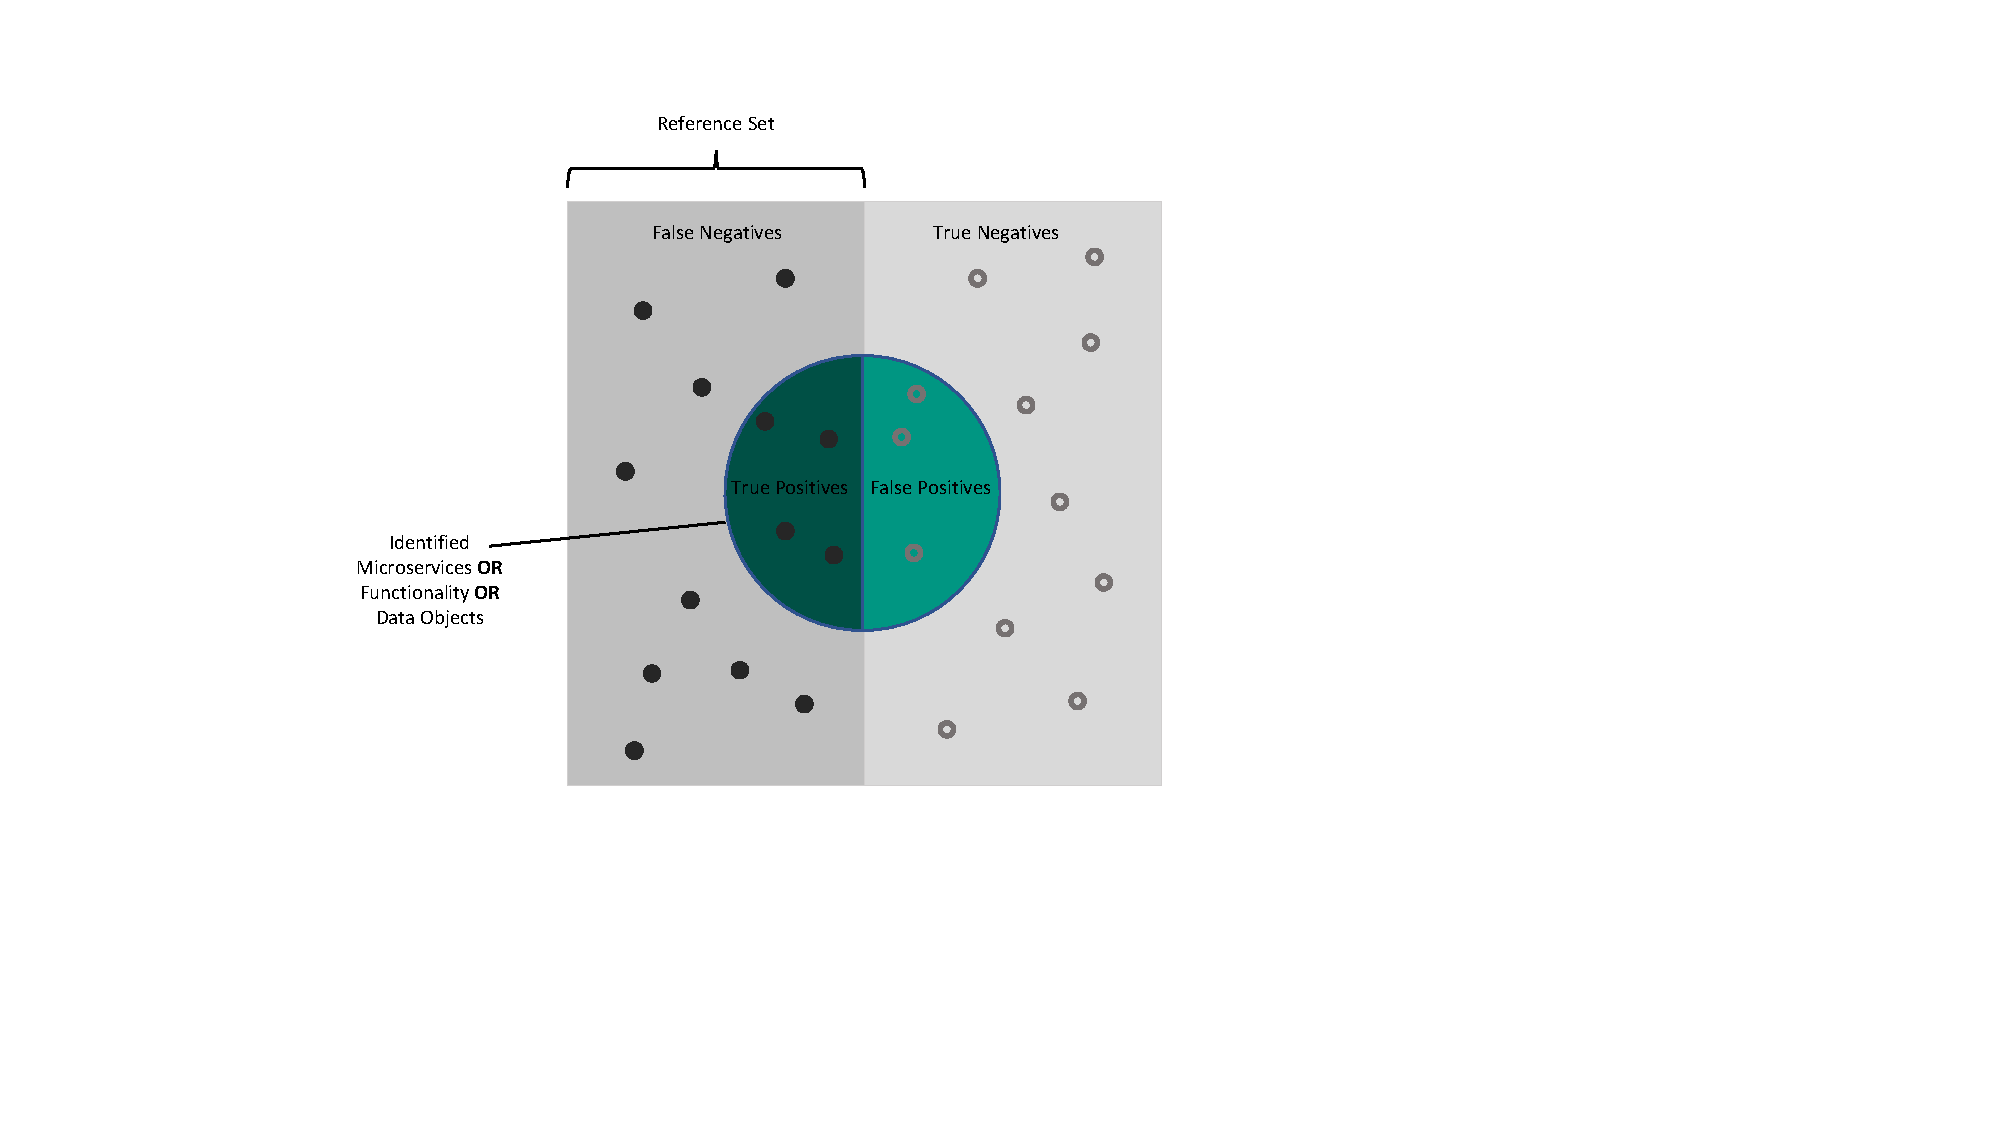
\includegraphics[ trim={7cm 5.5cm 8cm 0.5cm}, scale =1]{img/PrecisionRecall.pdf}
	\caption{Precision and Recall for Microservices}
	\label{fig:PrecisionRecall}
\end{figure}




\section{Evaluation Design}

\subsection{Evaluation Setup}
The primary goal of the evaluation is to determine the accuracy of the elaborated approach in order to answer \textbf{RQ1.3}. To achieve this, an \textit{Outcome Evaluation} is an appropriate method \cite{Evaluation}, as it shows how effective the approach is in terms of the expected results which are in this case adequate microservices. Therefore, the approach is applied to \textit{CoCoME} and the outcome is compared to two reference sets. \\
\textit{CoCoME} was initiated in a GI Dagstuhl research seminar as a community case study for software architecture, modelling and analysis.
In recent years, it has been applied in various areas as a demonstrator for software evolution methods\cite{CoCoMETechnical}. \textit{CoCoME} is structured like a typical, distributed and component-based information system and is therefore well suited as a demonstrator for this new type of software evolution - the migration to a microservice-based software architecture. 




\subsection{Reference Sets}
\label{sec:Evaluation:ReferenceSets}
To evaluate the approach, the identified set of microservices (cf. Sec.\ref{sec:Evalutation:Results}) is compared to two alternative decompositions of CoCoME: First, a decomposition proposed in the paper \textit{Identifying Microservices Using Functional Decomposition} \cite{FunctionalDecompositionHeinrich} and second, a set of microservices which we manually identified. \\

\noindent
\textbf{Reference Set 1: Functional Decomposition Approach} \\
\textit{Identifying Microservices Using Functional Decomposition} \cite{FunctionalDecompositionHeinrich} is a systematic approach to find an appropriate division of a system into microservices. This paper emerged as a result of the collaboration of the Academic College Tel-Aviv Yafo, the Karlsruhe Institute of Technology and the Southwest University China and uses CoCoME as demonstrator as well.\\
As depicted in Sec.\ref{sec:stateOfTheArt:approaches}, Tyszberowicz \textit{et al.} utilize the use case specifications of CoCoME \cite{CoCoMEOld} as input for their decomposition approach. Several external tools are used to extract verbs an nouns from the use cases that serve as \textit{system operations} and \textit{state variables}. Irrelevant nouns, verbs and synonyms are eliminated via brainstorming. The relationships between the aforementioned concepts are stored in a relation table. A relation exists, if a \textit{system operation} reads or updates a \textit{state variable}. Thereupon, the relation table is visualized as a weighted graph, which enables the identification of clusters of dense relationships. Each cluster serves as a microservice candidate.\\
As mentioned in Sec.\ref{sec:stateOfTheArt:comparison}, the compulsory and non-trivial revision of nouns and verbs to eliminate synonyms etc. is a substantial disadvantage.\\
Regarding the evaluation, Tyszberowicz \textit{et al.} claim that their approach identifies good microservices for a microservice-based system decomposition of CoCoME. The aforementioned evaluation includes a comparison to three independent software projects that implemented CoCoME. Two groups identified, apart from the naming, a similar set of microservices. The third group identified a more detailed decomposition of CoCoME, but a revision reveals that the additional microservices are only a refinement of the proposed microservices. \\
However, the evaluation lacks profundity: Microservices are only compared on a more abstract level, since it is not checked whether functionality and data objects are assigned to the correct microservice. The following microservices are identified: 



\begin{multicols}{2}
	\textbf{Sale}
	\begin{flushleft}
		\begin{itemize}[noitemsep]
			\item Handle Sale
			\item Handle Payment
			\item Identify stock Item
			\item \textbf{Data objects}: -  
		\end{itemize}
	\end{flushleft}
	
	
	\vfill
	\columnbreak
	\textbf{ProductList}
	\begin{flushleft}
		\begin{itemize}[noitemsep]
			\item Create orders
			\item Change price
			\item \textbf{Data Objects}: product
			
			
		\end{itemize}
	\end{flushleft}
	
\end{multicols}




\begin{multicols}{2}
	\textbf{StockOrder}
	\begin{flushleft}
		\begin{itemize}[noitemsep]
			\item Create stock report
			\item Handle inventory
			\item \textbf{Data objects}: stockItem, order
		\end{itemize}
	\end{flushleft}
	
	
	\vfill
	\columnbreak
	\textbf{Reporting}
	\begin{flushleft}
		\begin{itemize}[noitemsep]
			\item Create delivery report
			\item Handle deliveries
			\item \textbf{Data Objects}: - 
			
		\end{itemize}
	\end{flushleft}
\end{multicols}



\noindent
\textbf{Reference Set 2: Manual Decomposition} \\
In the course of this thesis, we implemented a microservice-based version of CoCoME. The microservice identification process itself was terminated before the literature review for the thesis started. Moreover, we were not aware of the microservice decomposition proposed by Tyszberowicz \textit{et al.} \cite{FunctionalDecompositionHeinrich} by the time we identified possible microservice candidates. Therefore, the process was non-biased. \\
The identification process itself was conducted manually and supported by the previous knowledge of the CoCoME domain. Once more, the time consuming and difficult identification process clarified the necessity of a structured and formal approach to identify microservices. Beside the use case specification, we used a monolithic implementation of CoCoME (the Hybrid Cloud-based Variant \cite{CoCoMETechnical}) as additional information resource to discover requirements, functionality and dependencies. Subsequently, the system was decomposed into loosely coupled and highly cohesive microservices. \\
The following four microservices were identified:




\begin{multicols}{2}
	\textbf{Stores- and Sale}
	\begin{flushleft}
		\begin{itemize}[noitemsep]
			\item Handle sale
			\item Handle payment
			\item Manage express checkout
			\item Exchange products
			\item Identify stock items
			\item Handle inventory
			\item Change price
			\item Handle stores
			\item Handle enterprises
			\item Handle deliveries
			\item \textbf{Data objects}: stockItem, store, enterprise
		\end{itemize}
	\end{flushleft}
	
	
	\vfill
	\columnbreak
	\textbf{Product}
	\begin{flushleft}
		\begin{itemize}[noitemsep]
			\item Show products
			\item Create products
			\item Show suppliers
			\item Create suppliers
			\item \textbf{Data Objects}: product, supplier
		
		
		\end{itemize}
	\end{flushleft}

\end{multicols}




\begin{multicols}{2}
	\textbf{Order}
	\begin{flushleft}
		\begin{itemize}[noitemsep]
			\item Show orders
			\item Create orders
			\item \textbf{Data objects}: order
		\end{itemize}
	\end{flushleft}
	
	
    	\vfill
	\columnbreak
	\textbf{Reports}
	\begin{flushleft}
		\begin{itemize}[noitemsep]
			\item Create delivery report
			\item Create stock report
			\item \textbf{Data Objects}: report  
	
		\end{itemize}
	\end{flushleft}
\end{multicols}





\noindent
\textbf{Differences between both sets} \\
The reference sets contain the same amount of microservices. Apart from the naming, those services are similar: One is responsible for the sale process, another one handles products, the third one is responsible for the orders and the last one is in charge of the reporting. \\
Nevertheless, the two differ from each other in regard to the functionality and data objects. Obviously, \textit{Reference Set 1} features nine functionalities and three data objects whereas \textit{Reference Set 2} contains 18 functionalities and seven data objects. It is important to note that all functionalities and data objects of the first reference set are part of the second one. Since the second reference set corresponds to a real implementation, it can be assumed that the first set is not complete. \\
Furthermore, both sets differ in the distribution of functionality and data objects among services. For instance, in \textit{Reference Set 1} the data object \textit{stockItem} is divided into the order microservice, whereas in \textit{Reference Set 2} it is divided into the sale's microservice. To provide another example, the functionalities \textit{Create Stock Report} and \textit{Create Delivery Report} are distributed differently: In the first reference set, \textit{Create Stock Report} is part of the \textit{Report} microservice and \textit{Create Delivery Report} is part of the order microservice whereas in the second reference set, both functionalities belong to the report service, which is more reasonable from the domain point of view. This example indicates a discrepancy between \textit{Reference Set 1} and \textit{Reference Set 2} where the latter corresponds to a real implementation. \\
Thus, a stronger focus is placed on the comparison with the second reference set.




\section{Evaluation Results}
\label{sec:Evalutation:PrecisionAndRecallMeasurement}
In this section, the precision and recall metric (cf. Sec.\ref{sec:Evaluation:Metrics:sPrecRecall}) for the results of the approach (cf. Sec.\ref{sec:SolutionApplication:ExtractMicroserviceCandidates}) is calculated using the reference sets described in Sec.\ref{sec:Evaluation:ReferenceSets}. 
For each reference set, the precision and recall instances are i) identified microservices, ii) identified functionality offered by a microservice and iii) identified data objects administered by a microservice. 

\subsection{Reference Set 1}

\textbf{Microservices} The approach identified three services, \textit{Microservice 1} is similar to \textit{Sale} and \textit{Microservice 2} is comparable to \textit{Reporting}. \textit{Microservice 3}, on the other hand, can neither be clearly assigned to \textit{StockOrder} nor to \textit{ProductList}, since it unites the functionalities of both. More specifically, \textit{Microservice 3} is a more coarse-grained microservice that consists of \textit{StockOrder} and \textit{ProductList}. Therefore it can be concluded that three out of four microservices were successfully identified, and none of the identified microservices are incorrect. 

\hspace{1cm}
\noindent
\begin{minipage}{.4\linewidth}
		\vspace{0.5cm}
	\flushleft

		
	$Recall_{microservice}=\dfrac{3}{4} = 0.75  $
		\vspace{0.5cm}
	
\end{minipage}%
\begin{minipage}{.5\linewidth}
	\vspace{0.5cm}
	\flushleft

		
	$Precision_{microservice}=\dfrac{3}{3} = 1  $
		\vspace{0.5cm}
	
\end{minipage}

\noindent
\textbf{Functionality} Since \textit{Microservice 3} consists of the microservices \textit{StockOrder} and \textit{ProductList}, functions that appear in this microservice and in either of the other two are regarded to be successfully identified. With this in mind, the results are as follows: The reference set counts nine functionalities. The approach identified 13 functionalities, from which five are assigned to the right service. Hence, the precision and recall values are:

\hspace{1cm}
\noindent
\begin{minipage}{.4\linewidth}
	\vspace{0.5cm}
	\flushleft
	
	
	$Recall_{functionality}=\dfrac{5}{9} \approx 0.56  $
	\vspace{0.5cm}
	
\end{minipage}%
\begin{minipage}{.5\linewidth}
	\vspace{0.5cm}
	\flushleft
	
	
	$Precision_{functionality}=\dfrac{5}{13} \approx 0.38  $
	\vspace{0.5cm}
	
\end{minipage}


\noindent
\textbf{Data Objects} Regarding \textit{Microservice 3}, the same line of reasoning is applied to the identified data objects: The reference set counts three data objects. The approach identified seven, from which 2 are assigned to the right service. In this case, the precision and recall values are:


\hspace{1cm}
\noindent
\begin{minipage}{.4\linewidth}
	\vspace{0.5cm}
	\flushleft
	
	
	$Recall_{dataObject}=\dfrac{2}{3} \approx 0.67  $
	\vspace{0.5cm}
	
\end{minipage}%
\begin{minipage}{.5\linewidth}
	\vspace{0.5cm}
	\flushleft
	
	
	$Precision_{dataObject}=\dfrac{2}{7} \approx 0.29  $
	\vspace{0.5cm}
	
\end{minipage}





\subsection{Reference Set 2}



\textbf{Microservices} As described in Sec.\ref{sec:Evaluation:ReferenceSets}, both reference sets contain similar microservices, which differ only by the names at microservice level. The functionalities and data objects, however, are different. Hence, the precision and recall value are identical in regard to identified microservices:

\hspace{1cm}
\noindent
\begin{minipage}{.4\linewidth}
	\vspace{0.5cm}
	\flushleft
	
	
	$Recall_{microservice}=\dfrac{3}{4} = 0.75  $
	\vspace{0.5cm}
	
\end{minipage}%
\begin{minipage}{.5\linewidth}
	\vspace{0.5cm}
	\flushleft
	
	
	$Precision_{microservice}=\dfrac{3}{3} = 1  $
	\vspace{0.5cm}
	
\end{minipage}

\noindent
\textbf{Functionality} Again \textit{Microservice 3} is considered to be a coarse grained union of the microservice \textit{Product} and \textit{Order}. In this case, the reference set counts 18 functionalities. The approach identified 13 functionalities, from which 12 are assigned to the right service. Hence, the precision and recall values are:

\hspace{1cm}
\noindent
\begin{minipage}{.4\linewidth}
	\vspace{0.5cm}
	\flushleft
	
	
	$Recall_{functionality}=\dfrac{12}{18} \approx 0.67  $
	\vspace{0.5cm}
	
\end{minipage}%
\begin{minipage}{.5\linewidth}
	\vspace{0.5cm}
	\flushleft
	
	
	$Precision_{functionality}=\dfrac{12}{13} \approx 0.92  $
	\vspace{0.5cm}
	
\end{minipage}


\noindent
\textbf{Data Objects} The reference set counts seven data objects. The approach identified seven, from which 5 are assigned to the right service. In this case, the precision and recall values are:


\hspace{1cm}
\noindent
\begin{minipage}{.4\linewidth}
	\vspace{0.5cm}
	\flushleft
	
	
	$Recall_{dataObject}=\dfrac{5}{7} \approx 0.71  $
	\vspace{0.5cm}
	
\end{minipage}%
\begin{minipage}{.5\linewidth}
	\vspace{0.5cm}
	\flushleft
	
	
	$Precision_{dataObject}=\dfrac{5}{7} \approx 0.71  $
	\vspace{0.5cm}
	
\end{minipage}

\section{Discussion of the Evaluation Results}
\label{sec:Evalutation:Results}
The measurement of the precision and recall metric in the previous section gives information about the accuracy of the approach. Each of the identified microservices is also represented in the reference sets, which leads to a maximum precision of \textit{1.0}. Due to the coarse-grained \textit{Microservice 3} the recall is at 0.75. Additionally, it has to be noticed that the approach does not produce any incorrect microservices. Regarding the functionality and data objects, the comparisons to the reference sets produces different values for recall and precision:\\

\noindent
Compared to the first reference set, the approach produces less 
satisfying values. Only about half (Recall = 0.56) of the functionality in the reference set is correctly identified.  In addition, only five out of 13 identified functionalities are assigned to the right service which leads to a small precision of 0.38. Regarding the data objects, the approach identifies two out of three correctly with an overall identification of seven data objects. Hence, the recall is at a satisfiable level of 0.67 but the precision is very low at 0.29. However, these non-satisfying values can be explained by the constitution of \textit{Reference Set 1} as described in Sec.\ref{sec:Evaluation:ReferenceSets}. The discrepancy between this reference set and a comparable implementation (\textit{Reference Set 2}) can explain the low recall value of the functionality. The incompleteness in regard to the data objects and the functionality explains the low precision values, as the approach identifies functionality and data objects which are not part of the reference set but obviously part of the CoCoME domain.\\

\noindent
Compared to the second reference set, the values for precision and recall are much better. Almost every identified functionality is assigned to the right microservice, which leads to a precision value of 0.92. Obviously the \textit{Reference Set 2} contains additional functionality that is not identified by the approach. As a consequence the recall value is not as high as the precision. However, it should be noted that the second reference set was created by using additional sources of information such as the source code whereas the approach only uses the provided use cases. With respect to the data objects, both precision and recall are at a satisfying value of 0.71. Finally, it has to be noticed that the approach does not identify any functionalities or data objects that are not part of \textit{Reference Set 2}. Only a few instances are assigned to wrong services. \\
Since a stronger focus is placed on the comparison with the second reference set, four our needs the accuracy of the elaborated approach is satisfying.
 






\section{Threats to Validity}
\label{sec:Evalutation:ThreatsToValidity}
To assess the overall validity of the evaluation results it is necessary to asses threats to the internal and external validity. 


\subsection{Internal Validity}
Internal validity describes to what extend the evaluation allows unfounded results, usually as a result of systematic errors and bias \cite{Validity}. \\
First of all, \textit{Reference Set 2} is based on our own implementation. We do not claim that this implementation represents the best or the only way to decompose CoCoME into appropriate microservices. However, the identification process was based on a sufficient knowledge about the CoCoME domain and the microservice topic. Hence, we claim that \textit{Reference Set 2} can be used to determine the accuracy. However, to eliminate final doubts, either another independent reference set should be consulted or the existing results should be reviewed by unbiased domain experts. \\
In order to compare the results with the reference sets, it is necessary to identify similar functionalities and data objects (cf. Sec.\ref{sec:SolutionApplication:ExtractMicroserviceCandidates}) that appear in each of them. We tried to avoid any biased fitting between the available instances in the reference sets and the result of the approach. However, this cannot be entirely ruled out.\\
Another threat to the validity is the claim that \textit{Microservice 3} consists of the microservices \textit{Order} and \textit{Product}. Functions and data object that appear in \textit{Microservice 3} are regarded to be successfully identified if they are in either of the two reference microservices. Strictly speaking, only two of the four reference services are identified by the approach. Consequently, all functionalities and data objects assigned to \textit{Microservice 3} would be false positives. This, however, distorts the result in the same negative way, since most of the functions and data objects were assigned correctly, but to the coarse-grained \textit{Microservice 3}.




\subsection{External Validity}
In contrast, external validity describes whether the evaluation results can be generalized and applied to other contexts \cite{Validity}. That is to say, the approach also produces good microservice candidates for systems that are not in the context of a supermarket chain like CoCoME. \\
During the development of the approach, no domain restrictions were wittingly enforced. All assumptions were made with the intention of being context-independent. Further, \textit{CoCoME} is structured like a typical, distributed and component-based information system. It is therefore to be expected that the approach also produces adequate results for other information systems. \\
Besides all the precautions, it is still possible that a fitting between CoCoME and the developed approach has happened. It is therefore necessary to apply the approach to other systems in different context to validate it's generality.









\chapter{Discussion}
\label{ch:Discussion}
%TODO Chapter beschreiben

\section{Using Use Cases as Input}
- Das Transformieren mit Data Needs ist nicht komplett trivial --> Falls aber BPMN als Input bereits vorliegen, wäre es perfekt

\section{Control Flow Graph...}
- Bei direkt verbundenen ist es eindeutig. Bei Parallel Gateway auch, da beide gleich oft ausgeführt werden. Problematisch wird es bei XOR, da man nicht weiß, welche der wege mit welcher Wahrscheinlichkeit genommen werden



Rein das wir kein extra DFD wollen als inpout sonder einfachen input verarbeiten --> mehr testen und eventuell doch den DFD extra extrahieren


Sind denn alle zugriffe gleichwertig? Gbt es unterschiede
\chapter{Conclusion}
\label{ch:Conclusion}
This thesis focused on finding a formal way to extract microservices using clustering on control flow and data flow. Chapter \ref{ch:Introduction} motivates the topic and poses the research questions. In Chapter \ref{ch:background}, the monolithic software architecture and the microservice architecture is introduced and shortly compared. Further, challenges and benefits of the microservice architecture are outlined. Also, this chapter introduces use cases and the \textit{Business Process and Model Notation (BPMN)}, which is a graph oriented language to describe business processes. Chapter \ref{ch:CoCoME} presents \textit{CoCoME}, the running example used to evaluate the approach. \textit{CoCoME} is a community case study and has recently been used in other projects to evaluate the results of microservice identification approaches. The current state of the art is introduced in Chapter \ref{ch:StateOfTheArt}, which provides the formal answer to \textbf{RQ1.1}: Several promising approaches and attempts to extract microservices are identified. Most of them require either a vast amount of initial input in form of diagrams, log files, graphs etc. or they require non-trivial user interaction during the extraction process. Also, some approaches cannot be applied to greenfield applications, as they need existing source code or at least a the change history of the software development process. However, a main objective was to identify microservice candidates without detailed know-how and manual effort which non of them can satisfy. \\
To answer \textbf{RQ1.2}, Chapter \ref{ch:Solution} introduces the actual approach to identify microservices based on business process models.  The approach is divided in several steps, where each step is explained in a distinct section. First, the BPMN models are specified. Since CoCoME's systems specifications are given in form of detailed use cases, a transformation method is introduced to transform use cases in BPMN models. In the following, strategies to extract the data flow and the control flow of the BPMN models are explained. Subsequently, a procedure is explained to visualize the data and control flow information as two separate weighted graphs that represent the dependencies between either data objects or activities. The next step introduces a clustering algorithm that uses a fitness function to determine the fitness of a selected partition. This algorithm is applied to the graphs in order to identify high cohesive and loosely coupled activity and data object clusters. In the last steps of the approach, four different methods to match the activity and data clusters are presented, where each combined cluster corresponds to a possible microservice candidate. \\
Chapter \ref{ch:SolutionApplication} applies the approach to the running example. Chapter \ref{ch:Evalutation} introduces a \textit{GQM Plan} to answer \textbf{RQ1.3} efficiently. This includes the introduction of a metric and the presentation of two reference sets. Further, the results of the previous chapter are compared to the reference sets using the metric.


\section{Outcomes}


\vspace{0.5cm}
\par
\begingroup

\noindent
\textbf{RQ1: How to identify microservices based on the system specifications? }

\vspace{0.3cm}
\noindent
\textbf{Outcome:} To that end, an approach was elaborated that uses clustering on control flow and data flow extracted from BPMN models.

\endgroup
\vspace{0.5cm}


\vspace{0.5cm}
\par
\begingroup

\noindent
\textbf{RQ1.1: Which is an appropriate strategy to decompose a system into microservices? }

\vspace{0.3cm}
\noindent
\textbf{Outcome:} The control flow and the data flow are used to identify two separate sets of clusters: Activity clusters based on control flow dependencies and data object clusters based on data flow dependencies. Afterwards, both sets of clusters are matched in order to generate high cohesive and loosely coupled microservices. 

\endgroup
\vspace{0.5cm}

\vspace{0.5cm}
\par
\begingroup

\noindent
\textbf{RQ1.2: What formal approach can be constructed to identify possible microservices without detailed know-how and manual effort? }

\vspace{0.3cm}
\noindent
\textbf{Outcome:} The approach consists of nine steps. The system specifications are in form of BPMN 2.0 models and contain control flow and data flow information. The information is extracted and visualized as two weighted graphs. Subsequently, a generic algorithm identifies dense activity and data object cluster. Based on the data object access between activity and data object clusters, the clusters are finally matched. Still, the manual effort is not negligible as the approach is not yet implemented. However, no additional effort, know-how or user-interaction is necessary, as soon as the BPMN models are specified. 



\endgroup
\vspace{0.5cm}

\vspace{0.5cm}
\par
\begingroup

\noindent
\textbf{RQ1.3: What is the accuracy of the approach? }

\vspace{0.3cm}
\noindent
\textbf{Outcome:} The overall accuracy of the approach is satisfying. No false microservice was identified when applying the approach to CoCoME. Solely one of the identified microservices is more coarse-grained compared to the reference sets. In addition, most of the identified functionalities and data objects were allocated to the right service. 

\endgroup
\vspace{0.5cm}


\section{Discussion}
Using use cases as input causes some trouble as the transformation into BPMN models with data needs is not trivial. It rather requires manual effort to detect synonymous tasks and data objects among all use cases to prevent a distorted result. This stands opposite the main purpose of the approach which is to reduce the required manual work and effort. However, it would be very difficult to create an approach that is capable of handling every form of input. Consequently, the first step, which is specifying the BPMN models, should rather be considered as prerequisite of the approach instead of being part of it. In case the system specifications are given as BPMN models with accompanying data reads and writes, the approach gets by on a minimum amount of required expertise and effort. \\
Section \ref{sec:Solution:CreateGraphControl} introduces the creation of a graph based on the control flow information. Regarding possible alternatives in the control flow (XOR gateways), it was decided not to assess different choices in terms of different weighting. Yet, it is debatable whether this does not distort the actual control flow dependencies and consequently the results. Since the goal was not to identify perfect and fixed microservices, but to deliver candidates with little additional knowledge, this point is rather insignificant. \\
Another debatable topic is the equal weighting of all edges between activities. One can argue that some activities are more relevant and executed more often. For instance, the \textit{Sale} process is probably performed much more often than creating a new product. Hence, activities covering the \textit{Sale} process need to be connected using edges with higher weights to raise the probability of ending in the same service. However, this would require domain experts to judge the relevance of each activity, leading to a much more complex and user-interactive process. \\ 
Probably the most controversial issue is the identification of data flow dependencies (cf. Sec.\ref{sec:Solution:CreateGraphData}). As BPMN 2.0 is not capable to model the data flow but rather the data needs of the activities, it is necessary to extract data flow dependencies between two data object based on heuristics. However, these depend very much on the granularity of the BPMN models. The value for the parameter \textit{n} needs to be adapted to the granularity, where fine-grained business processes demand for a higher value and vice versa. Additionally, the approach may not produce satisfying results if the granularity varies, that is if some business processes are much more fine or coarse grained than others. Consequently, it is perhaps necessary to think about additional input: The BPMN models are still used to extract the control flow information and to create activity clusters. In regard to data clusters, it might be necessary to use actual data flow diagrams that represent the exact data flow dependencies in order to create the data object related graph. Although this increases the necessary amount of input, it might improve the quality of the identified microservices. It is worth mentioning that the approach itself only needs to be adapted at two positions: i) \textit{Extract Data Flow} and ii) \textit{Create a weighted Graph using Data Flow}, which both would be trivial steps if the input is expanded by data flow diagrams. \\
The evaluation also demonstrated how close the result is compared to an actual implementation. However, it shows how important a complete system specification is: The use case specification of CoCoME does not mention tasks like \textit{Create Store} or \textit{Create Products}. Consequently, the result does not contain these either. Since the approach requires no further human intervention, the input must be very precise and detailed.\\
The overall results are sophisticating. The identified microservice, including their functionalities and data objects are mostly correctly identified. Compared to the manual process as presented in Sec.\ref{sec:Evaluation:ReferenceSets} which took days, the approach presented requires only a few hours. 







\section{Limitations and Future Work}
Despite the overall satisfying results, the approach has its limitations. First of all, system requirements need to be transformed into BPMN 2.0 models with additional data needs. Even though the BPMN language is well known to describe business processes, the extension by the data objects is rather unusual. Hence, specifying those models might be a new task for the system designers.  \\
In addition, it needs to be verified whether the approach is capable to detect different granular microservices. For instance, small services like \textit{Order} and \textit{Product} are not identified by the approach, because it merges them to a more coarse-grained microservice which has approximately the size of the other identified services. In this case, further research on different clustering algorithms needs to be conducted. Also, it would be nice to choose the degree of granularity when applying the approach. The current algorithm is not capable of finding various decompositions of a graph that vary in size. \\
In addition, we presented a conceptual algorithm to match cluster by using merging but also splitting. This needs further attention as it might solve the issue of different granular microservices.  Above all, the currently used black box cluster matching process can lead to very large microservices, since only merging is used. Therefore, the conceptional white box clustering algorithm should be further investigated. \\
As already discussed in the previous section, the granularity of the BPMN models determines the choice of the parameter \textit{n}, which influences possible data object dependencies. 
Apart from the fact that a wrong choice of the parameter distorts the result, it is questionable to apply the approach to BPMN models of different granularity. In other words, the approach is able to handle either coarse-grained or fine-grained BPMN models, but not a mix of both. \\
The microservice candidates generated by the approach are not fix and ready to implement but should rather used as a recommendation to inspire the system architect. Additionally, microservices need a clear and well-defined external interface to provide shared functionality and data access to other services. This is not yet covered by the approach, although the information is already provided implicitly. 









%% --------------------
%% |   Bibliography   |
%% --------------------

%% Add entry to the table of contents for the bibliography
\printbibliography[heading=bibintoc]

%% ----------------
%% |   Appendix   |
%% ----------------
\appendix
%% LaTeX2e class for student theses
%% sections/apendix.tex
%% 
%% Karlsruhe Institute of Technology
%% Institute for Program Structures and Data Organization
%% Chair for Software Design and Quality (SDQ)
%%
%% Dr.-Ing. Erik Burger
%% burger@kit.edu
%%
%% Version 1.3.3, 2018-04-17

\iflanguage{english}
{\chapter{Appendix}}    % english style
{\chapter{Anhang}}      % german style
\label{ch:appendix}


%% -------------------
%% | Example content |
%% -------------------
\section{BPMN Models}
\label{sec:appendix:BPMN Models}
		
\setcounter{figure}{0}
		
%"l, b, r, t"
\begin{figure}[h!]
	\centering
	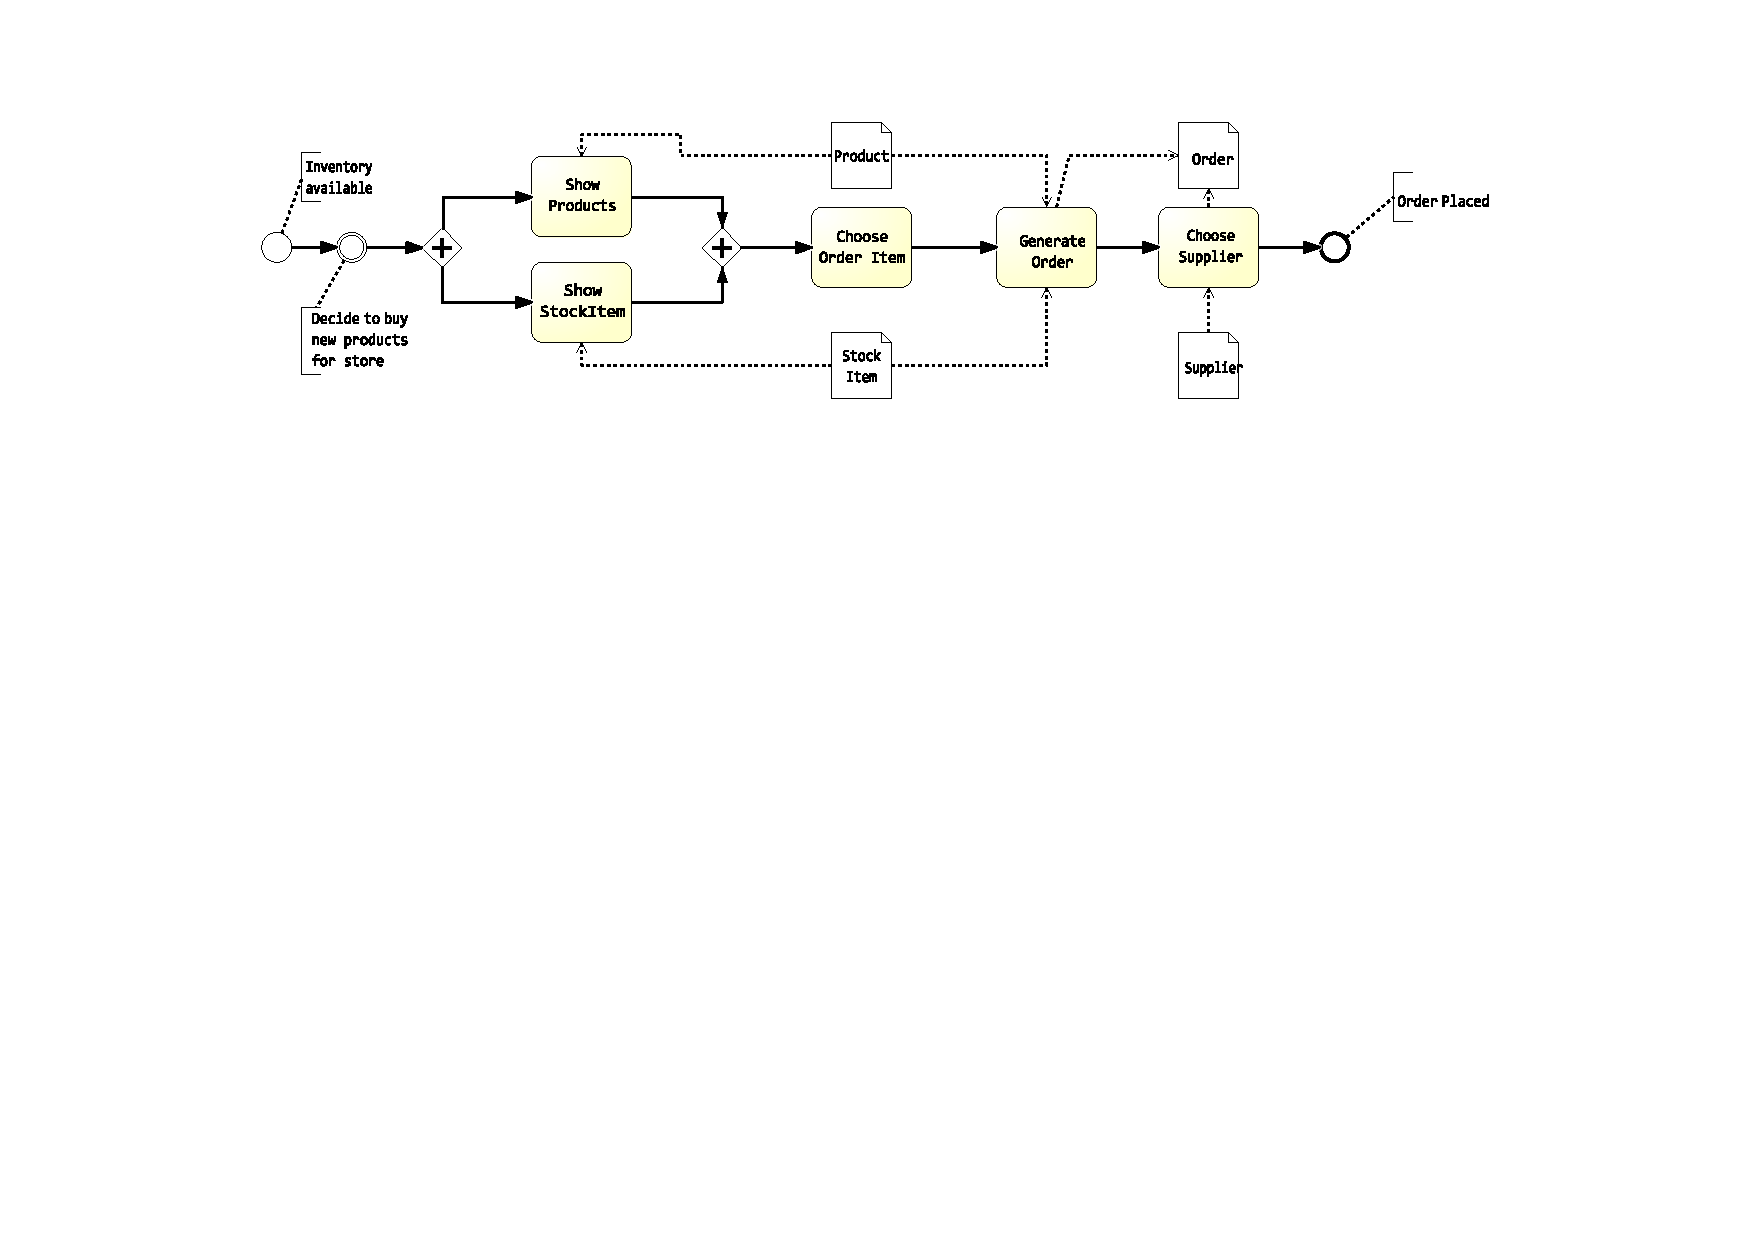
\includegraphics[width=\textwidth, trim={6cm 14cm 6cm 1cm}]{img/UC3.pdf}
	\caption{UC3 - Order Products}
	\label{fig:UC3}
\end{figure}


%"l, b, r, t"
\begin{figure}[h!]
	\centering
	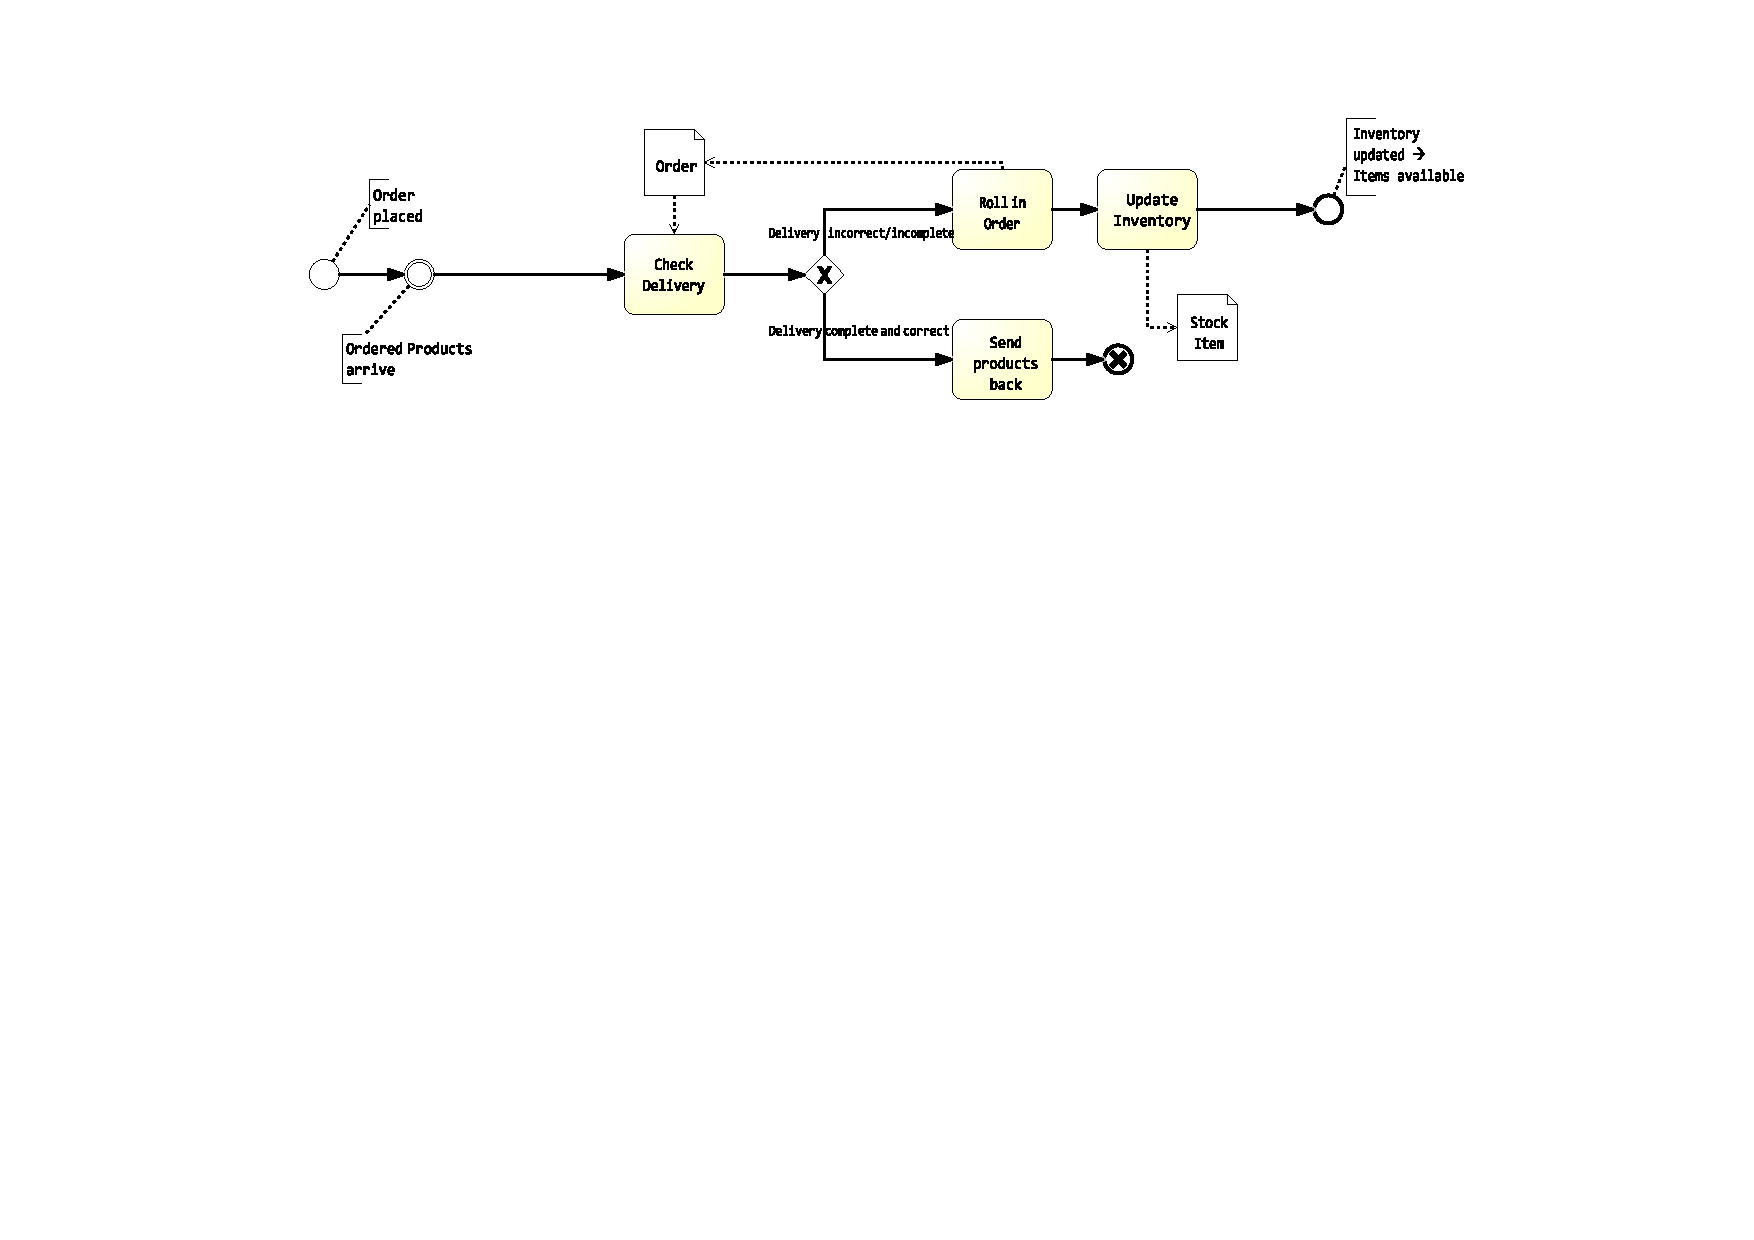
\includegraphics[width=\textwidth, trim={6.5cm 14cm 6cm 1cm}]{img/UC4.pdf}
	\caption{UC4 - Receive Ordered Products }
	\label{fig:UC4}
\end{figure}

\pagebreak

%"l, b, r, t"
\begin{figure}[h!]
	\centering
	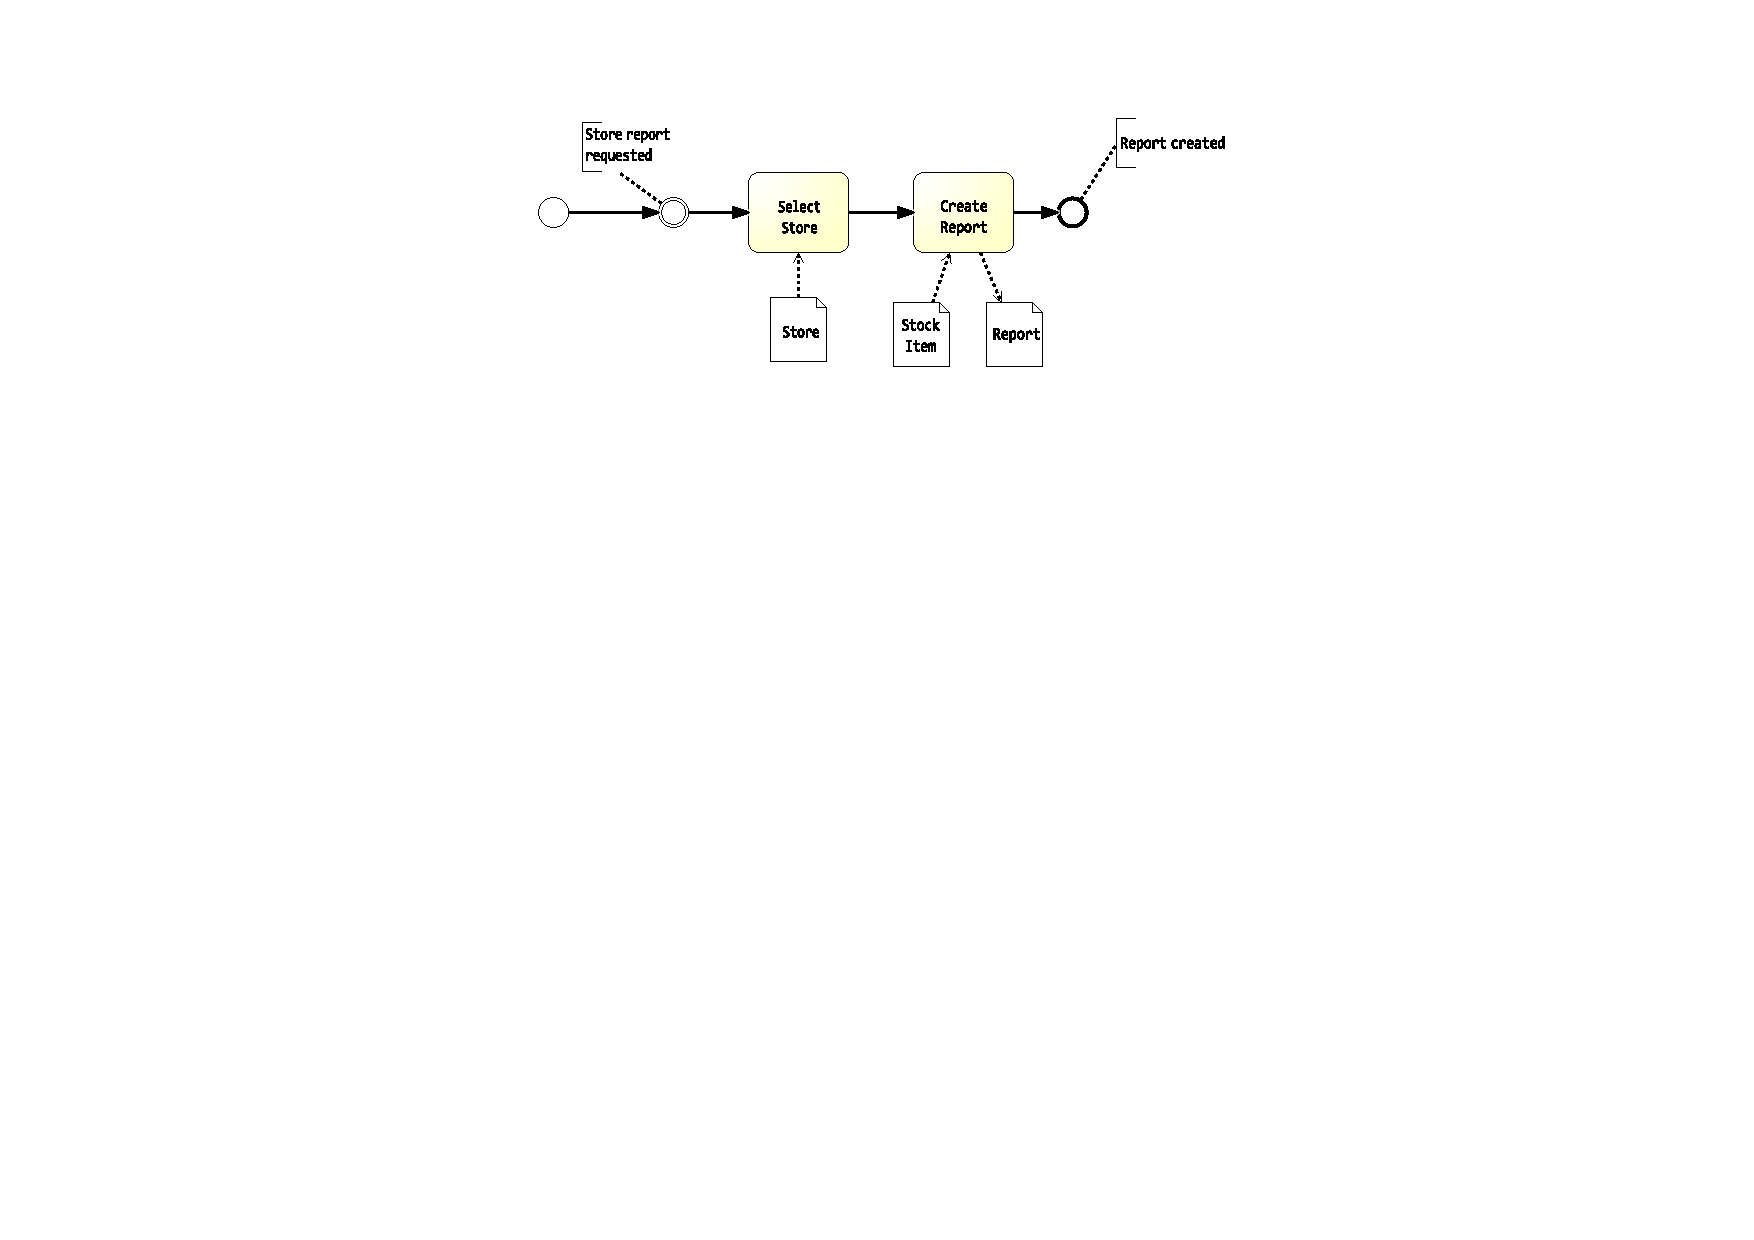
\includegraphics[width=\textwidth, trim={6cm 15cm 7cm 1cm}]{img/UC5.pdf}
	\caption{UC5 - Show Stock Reports }
	\label{fig:UC5}
\end{figure}

%"l, b, r, t"
\begin{figure}[h!]
	\centering
	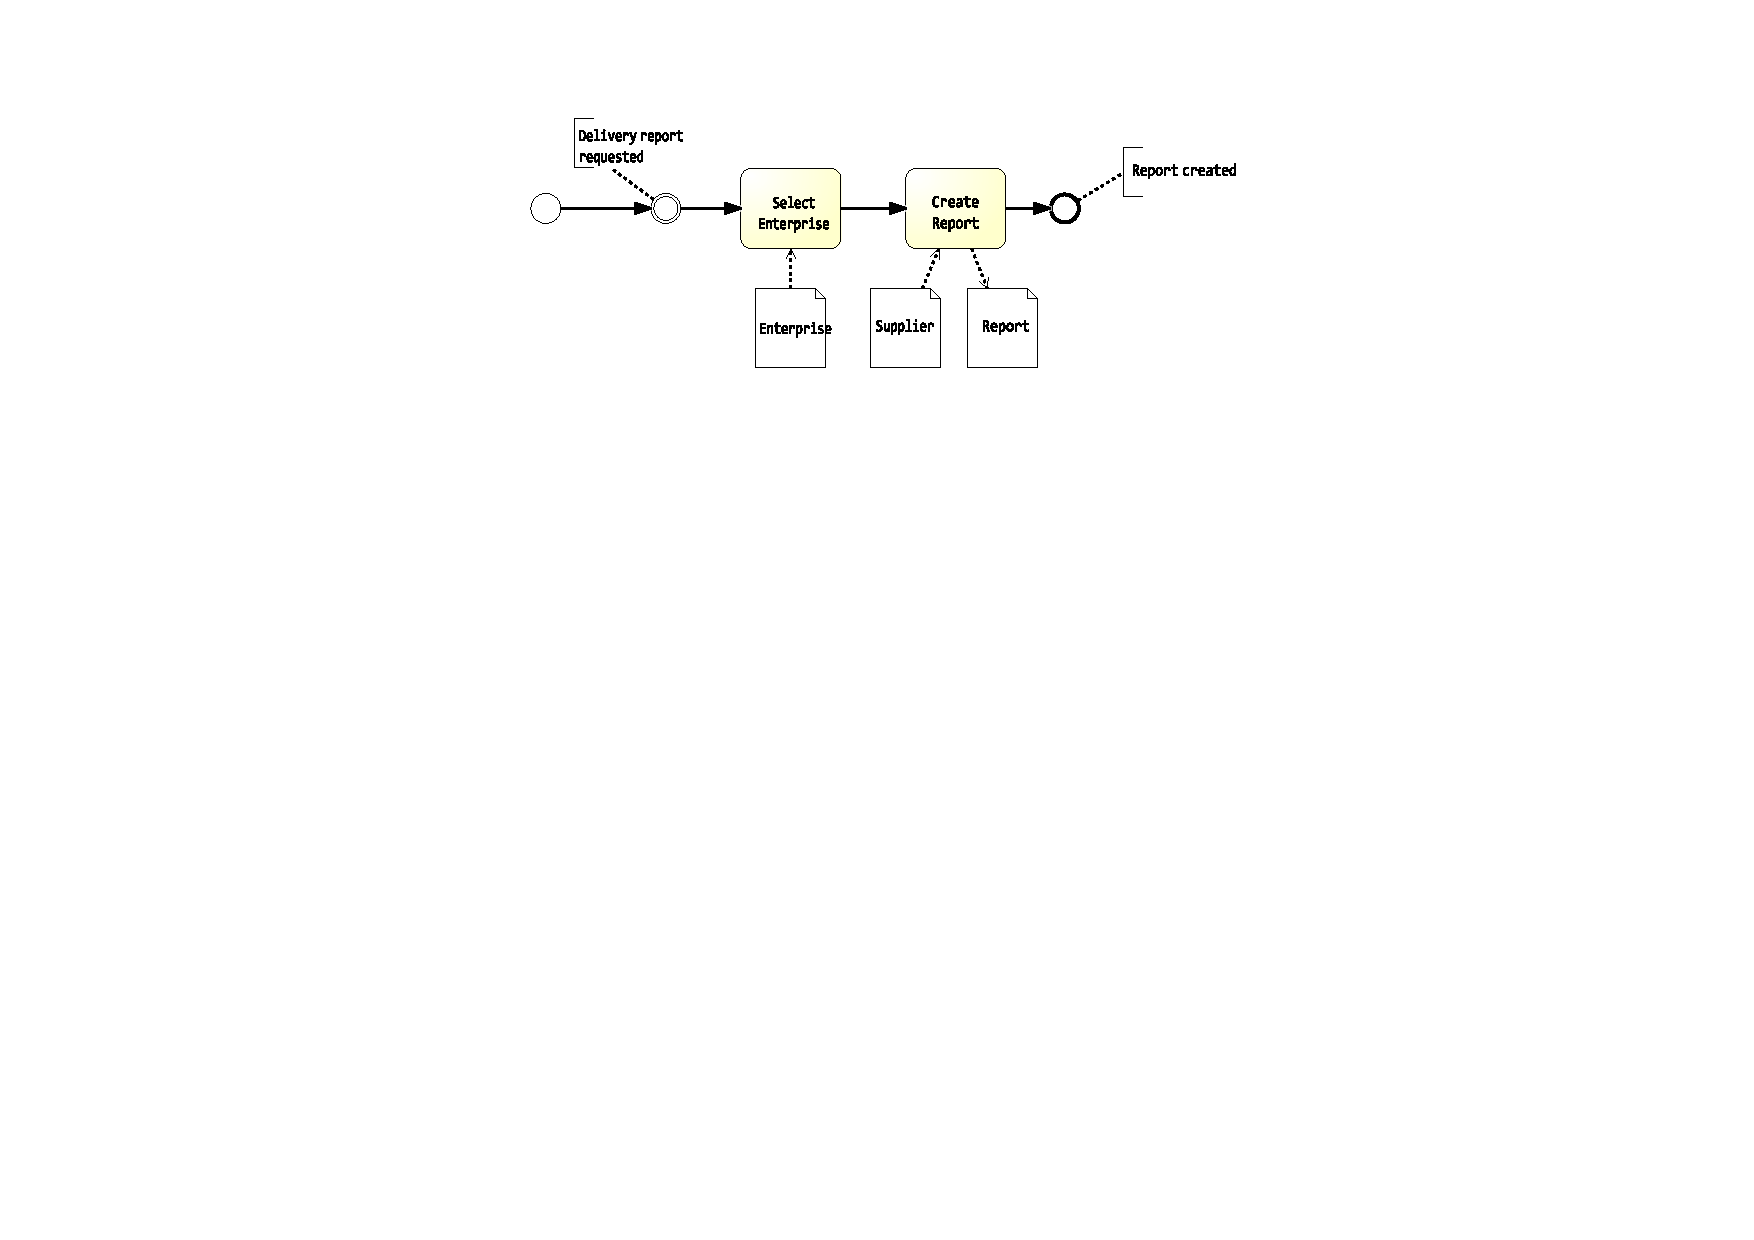
\includegraphics[width=\textwidth, trim={6cm 14.5cm 7cm 1cm}]{img/UC6.pdf}
	\caption{UC6 - Show Delivery Reports }
	\label{fig:UC6}
\end{figure}

%"l, b, r, t"
\begin{figure}[h!]
	\centering
	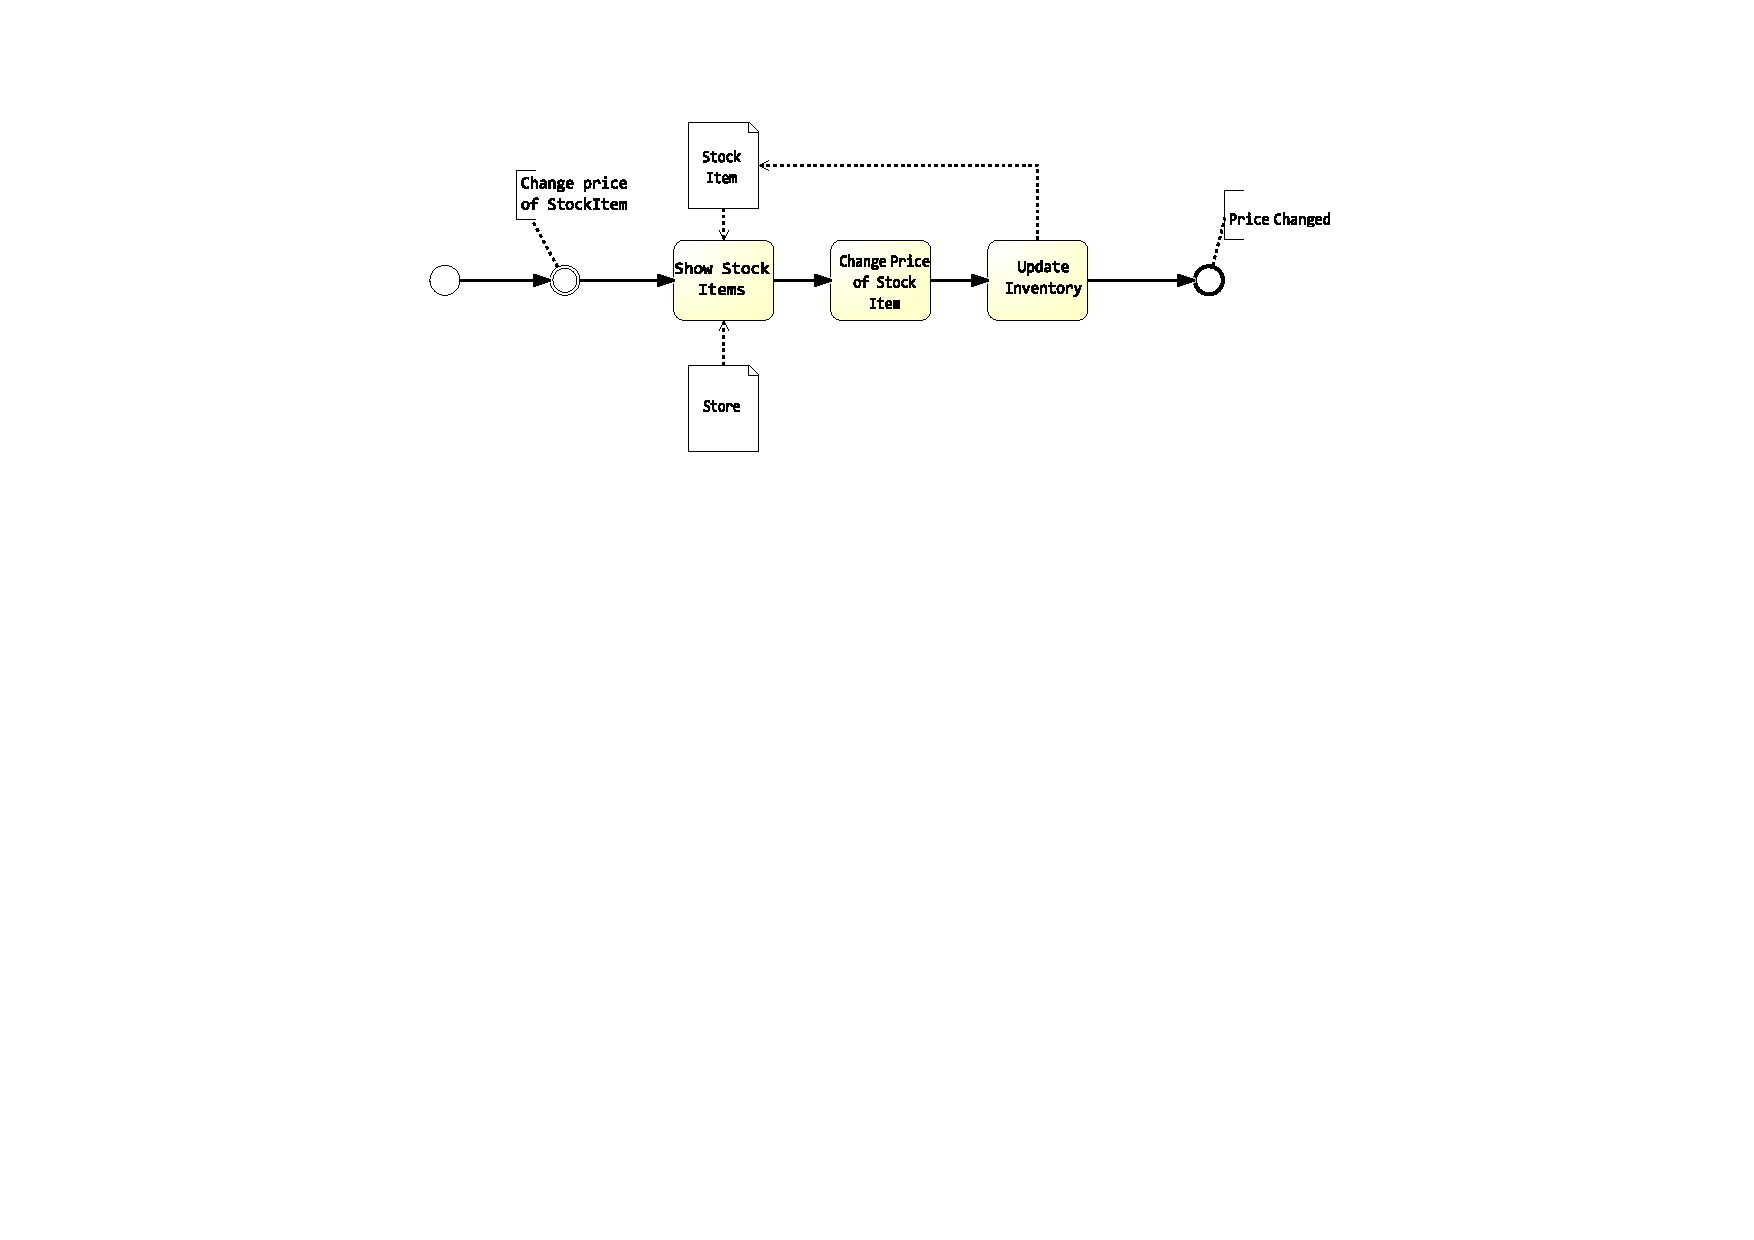
\includegraphics[width=\textwidth, trim={6cm 13cm 7cm 1cm}]{img/UC7.pdf}
	\caption{UC7 - Change Price }
	\label{fig:UC7}
\end{figure}

\clearpage

\section{Control Flow Diagrams}
\label{sec:appendix:ControlFlow}

%"l, b, r, t"
\begin{figure}[h!]
	\centering
	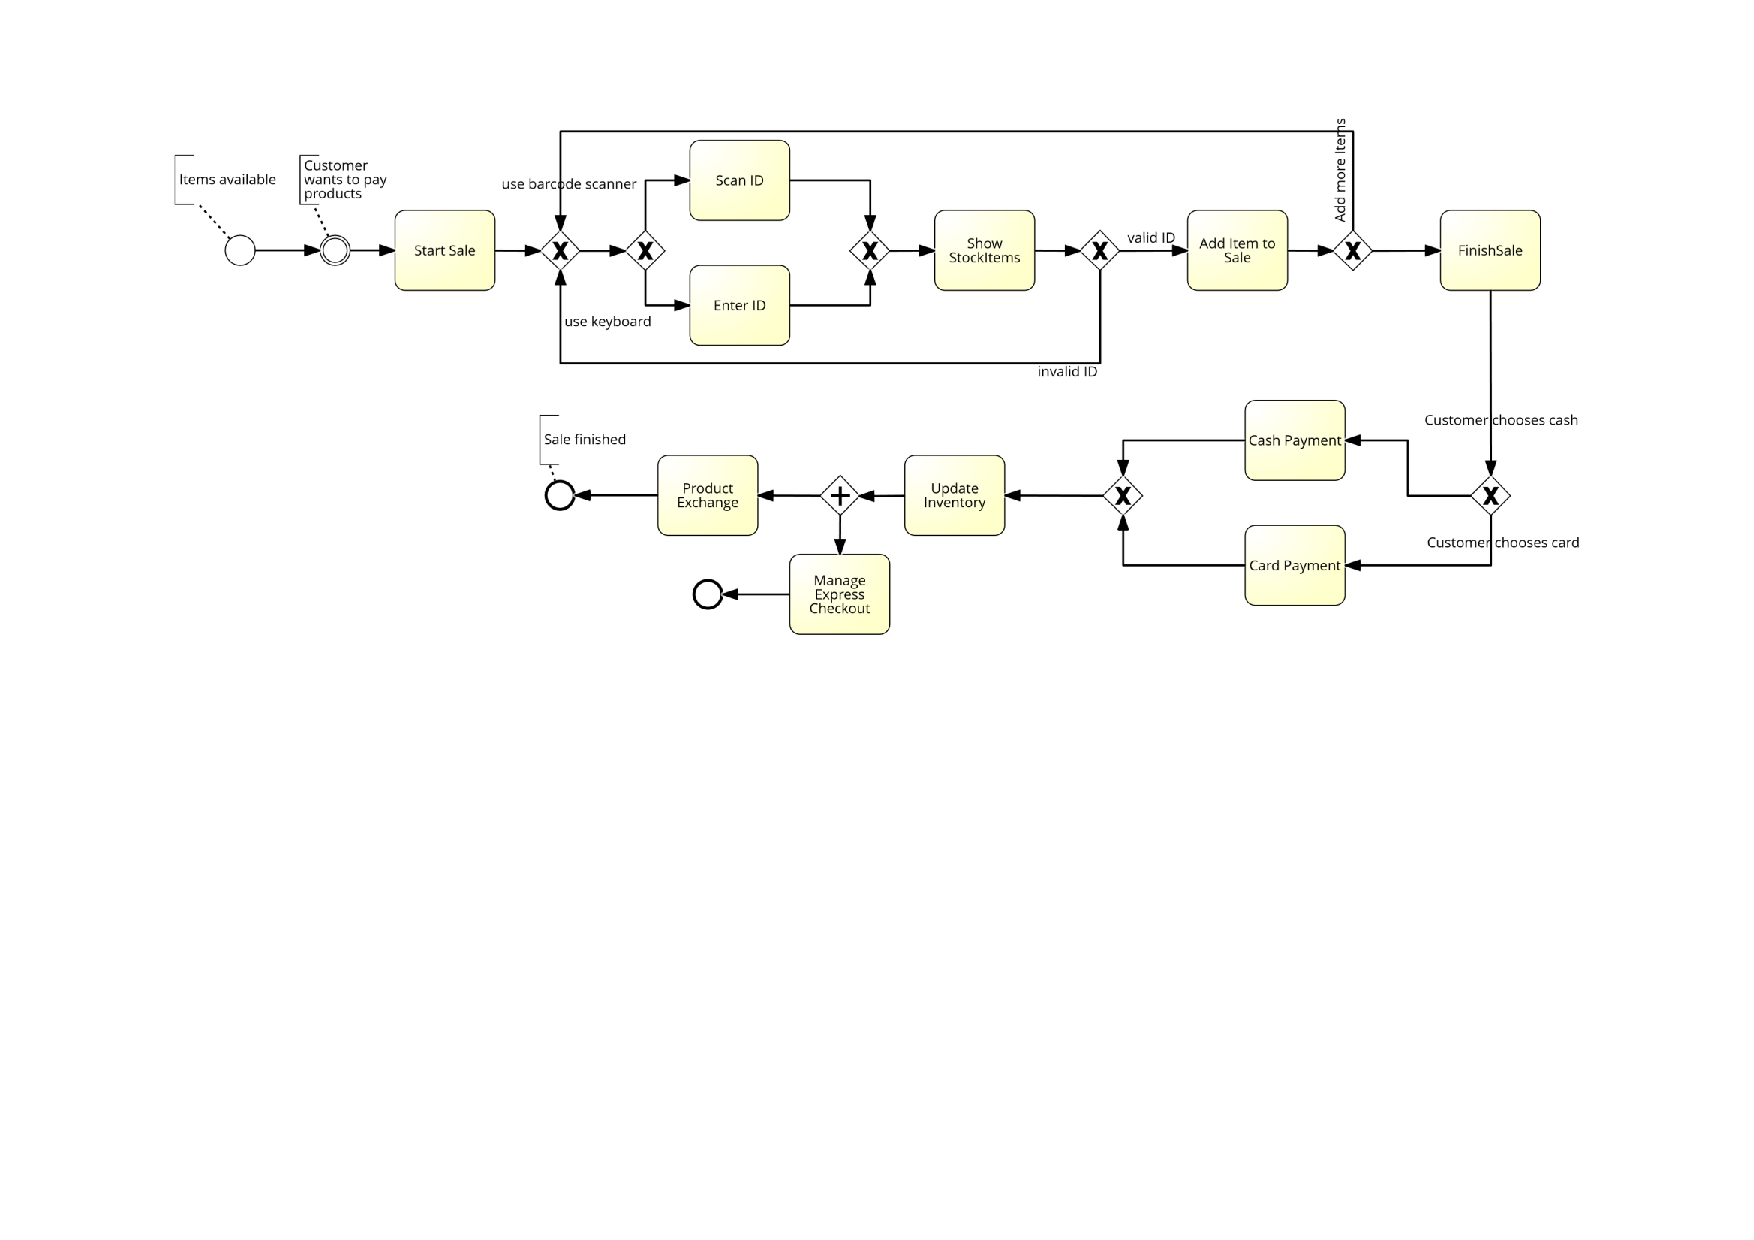
\includegraphics[width=\textwidth, trim={5cm 10cm 4cm 1cm}]{img/UC1Control.pdf}
	\caption{Control Flow UC1 - Start Sale}
	\label{fig:UC1Control}
\end{figure}


%"l, b, r, t"
\begin{figure}[h!]
	\centering
	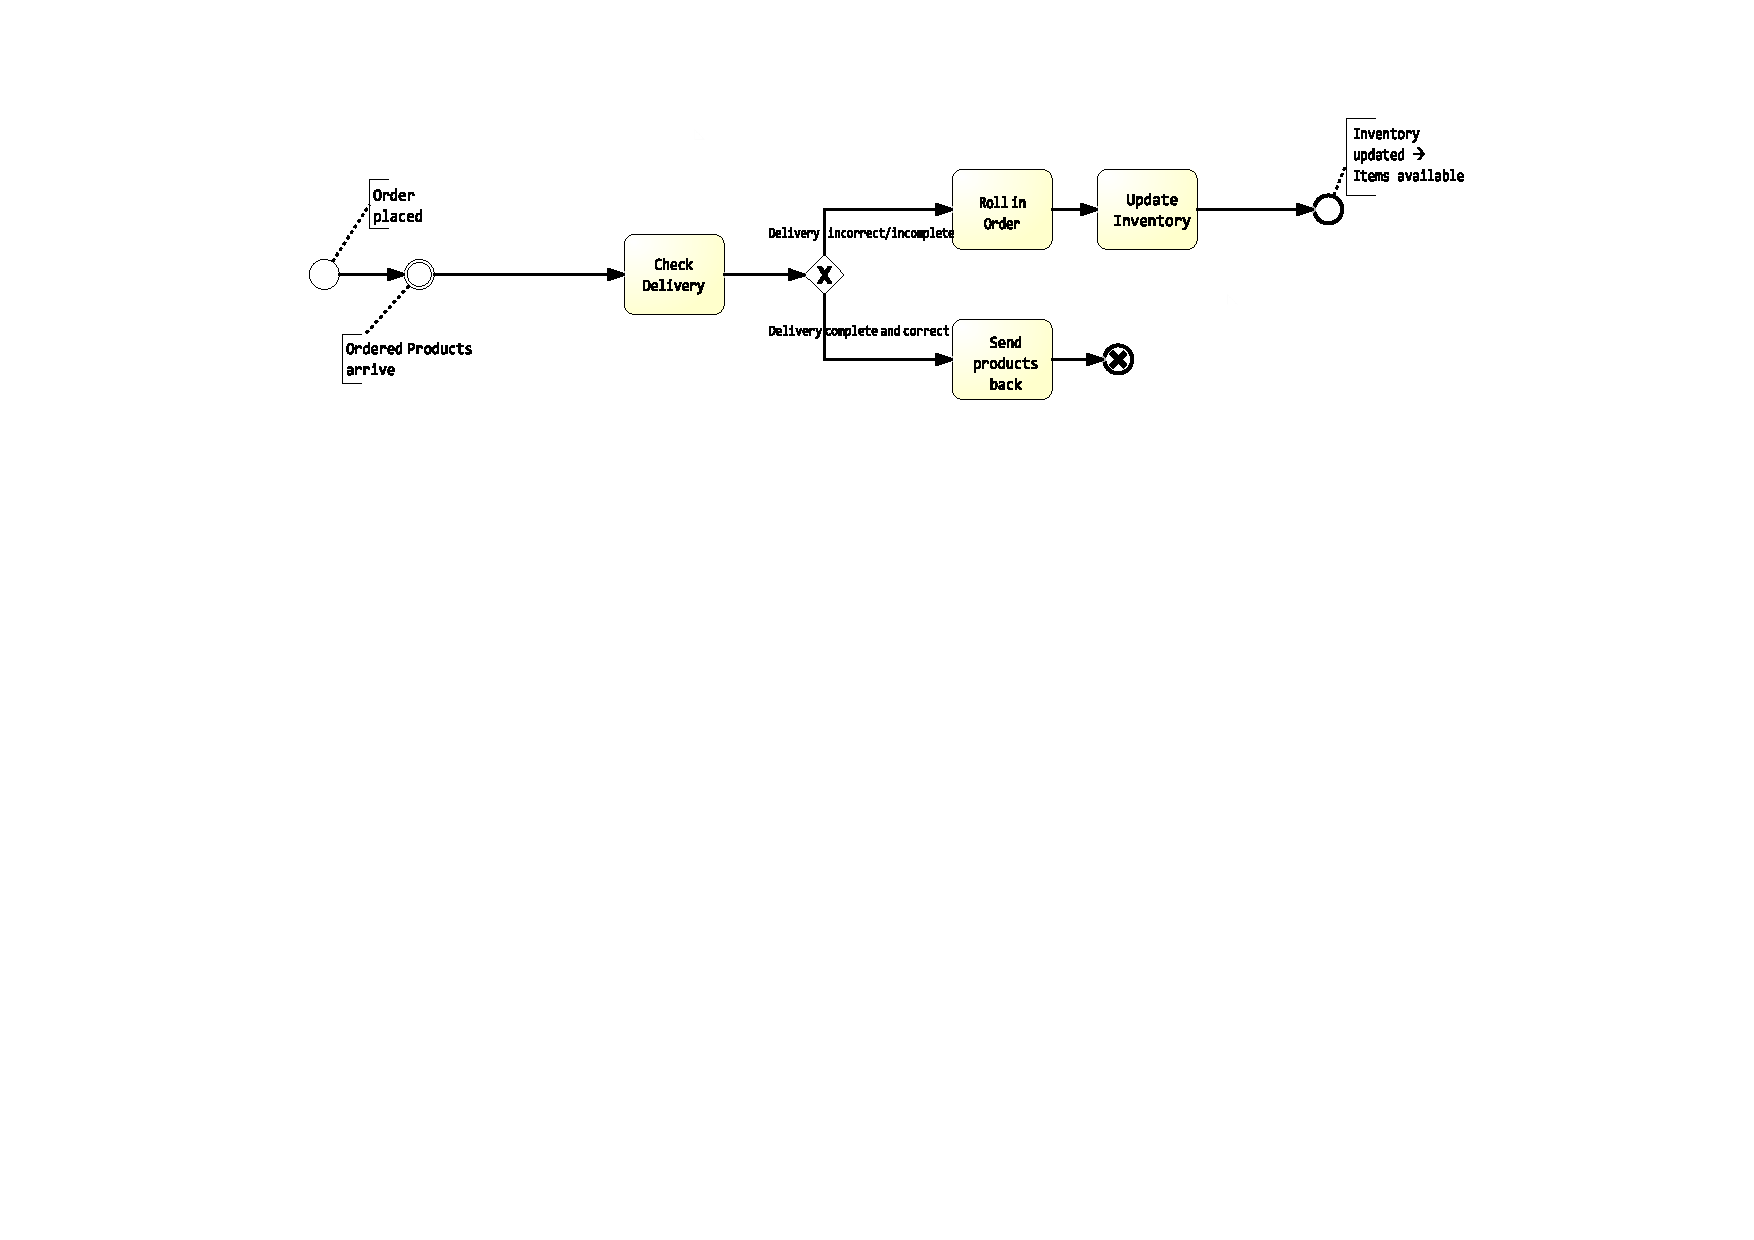
\includegraphics[width=\textwidth, trim={7cm 14cm 6cm 1cm}]{img/UC4Control.pdf}
	\caption{Control Flow UC4 - Receive Ordered Products }
	\label{fig:UC4Control}
\end{figure}

\pagebreak

%"l, b, r, t"
\begin{figure}[h!]
	\centering
	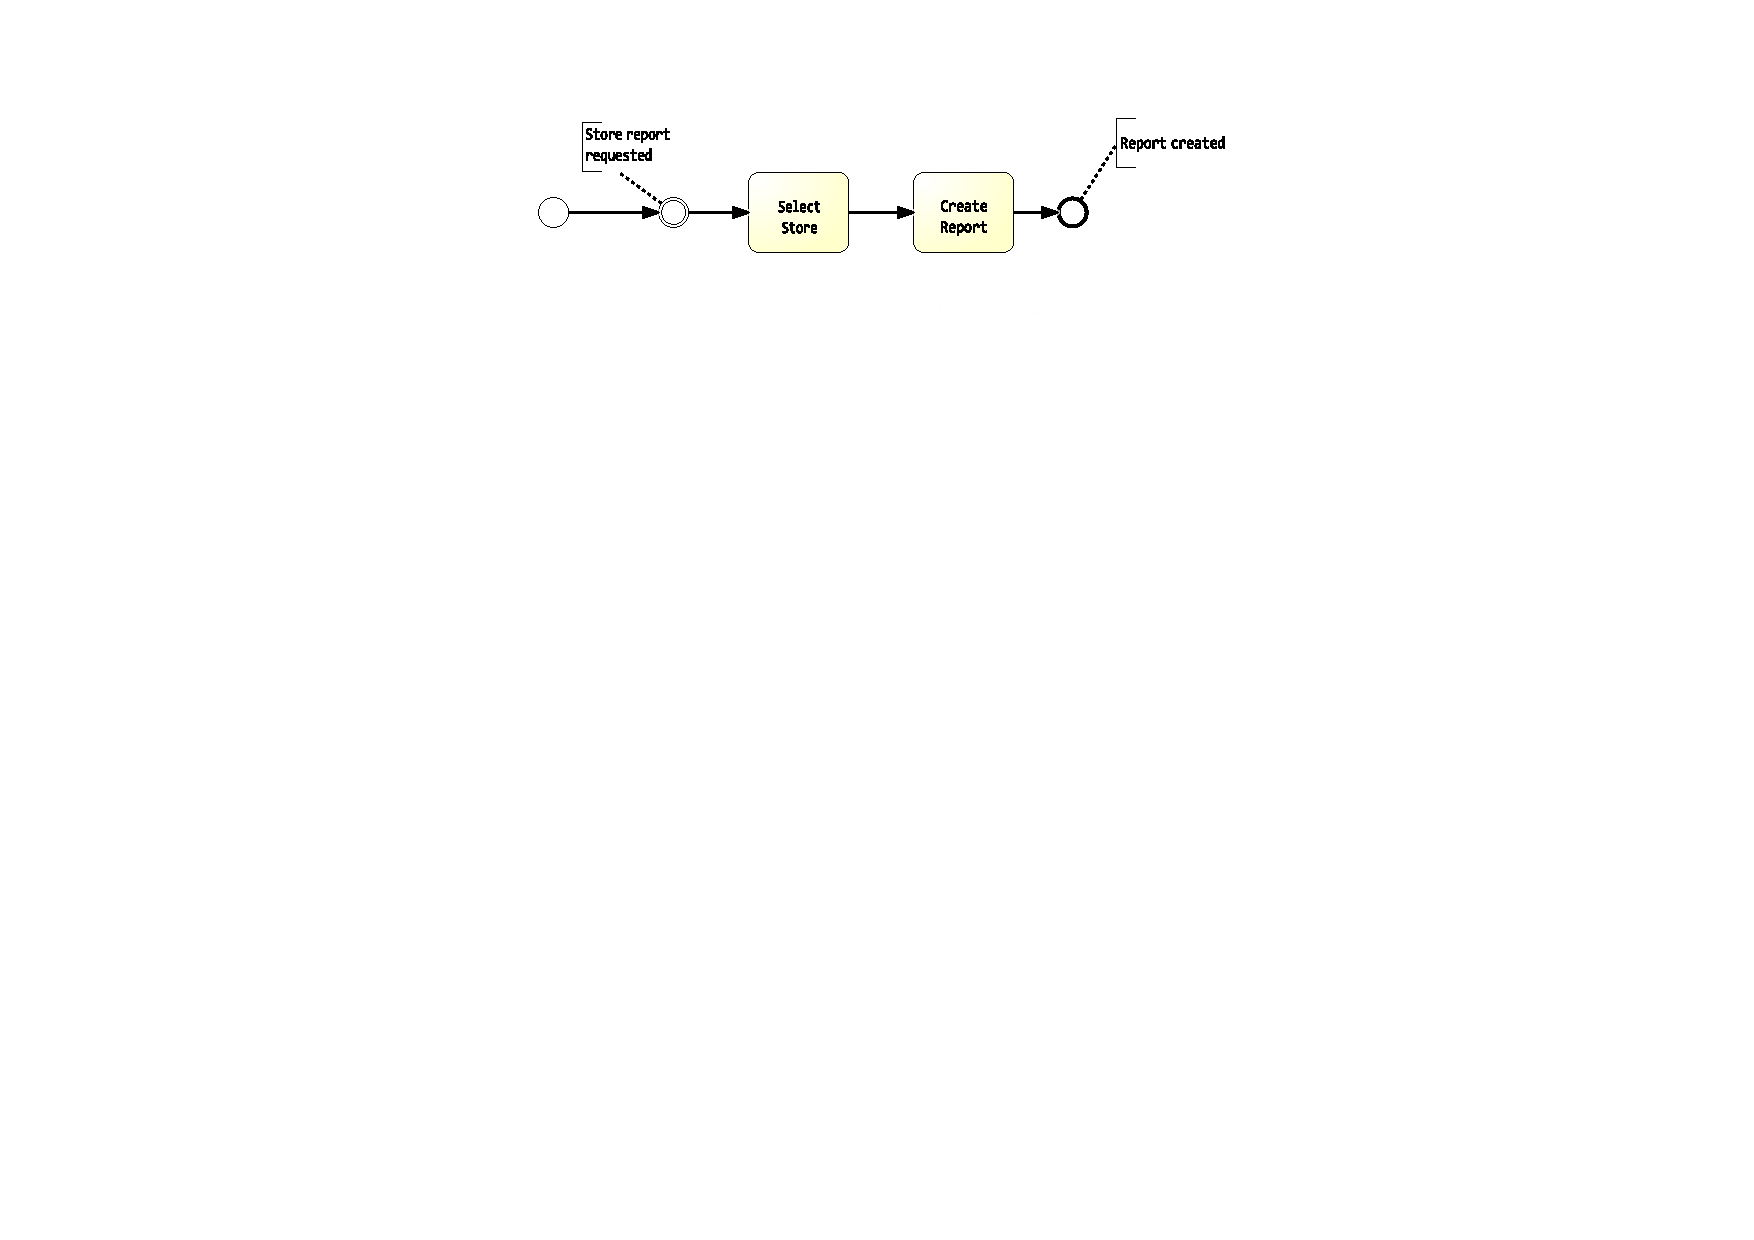
\includegraphics[width=\textwidth, trim={6cm 16.5cm 7cm 1cm}]{img/UC5Control.pdf}
	\caption{Control Flow UC5 - Show Stock Reports }
	\label{fig:UC5Control}
\end{figure}

%"l, b, r, t"
\begin{figure}[h!]
	\centering
	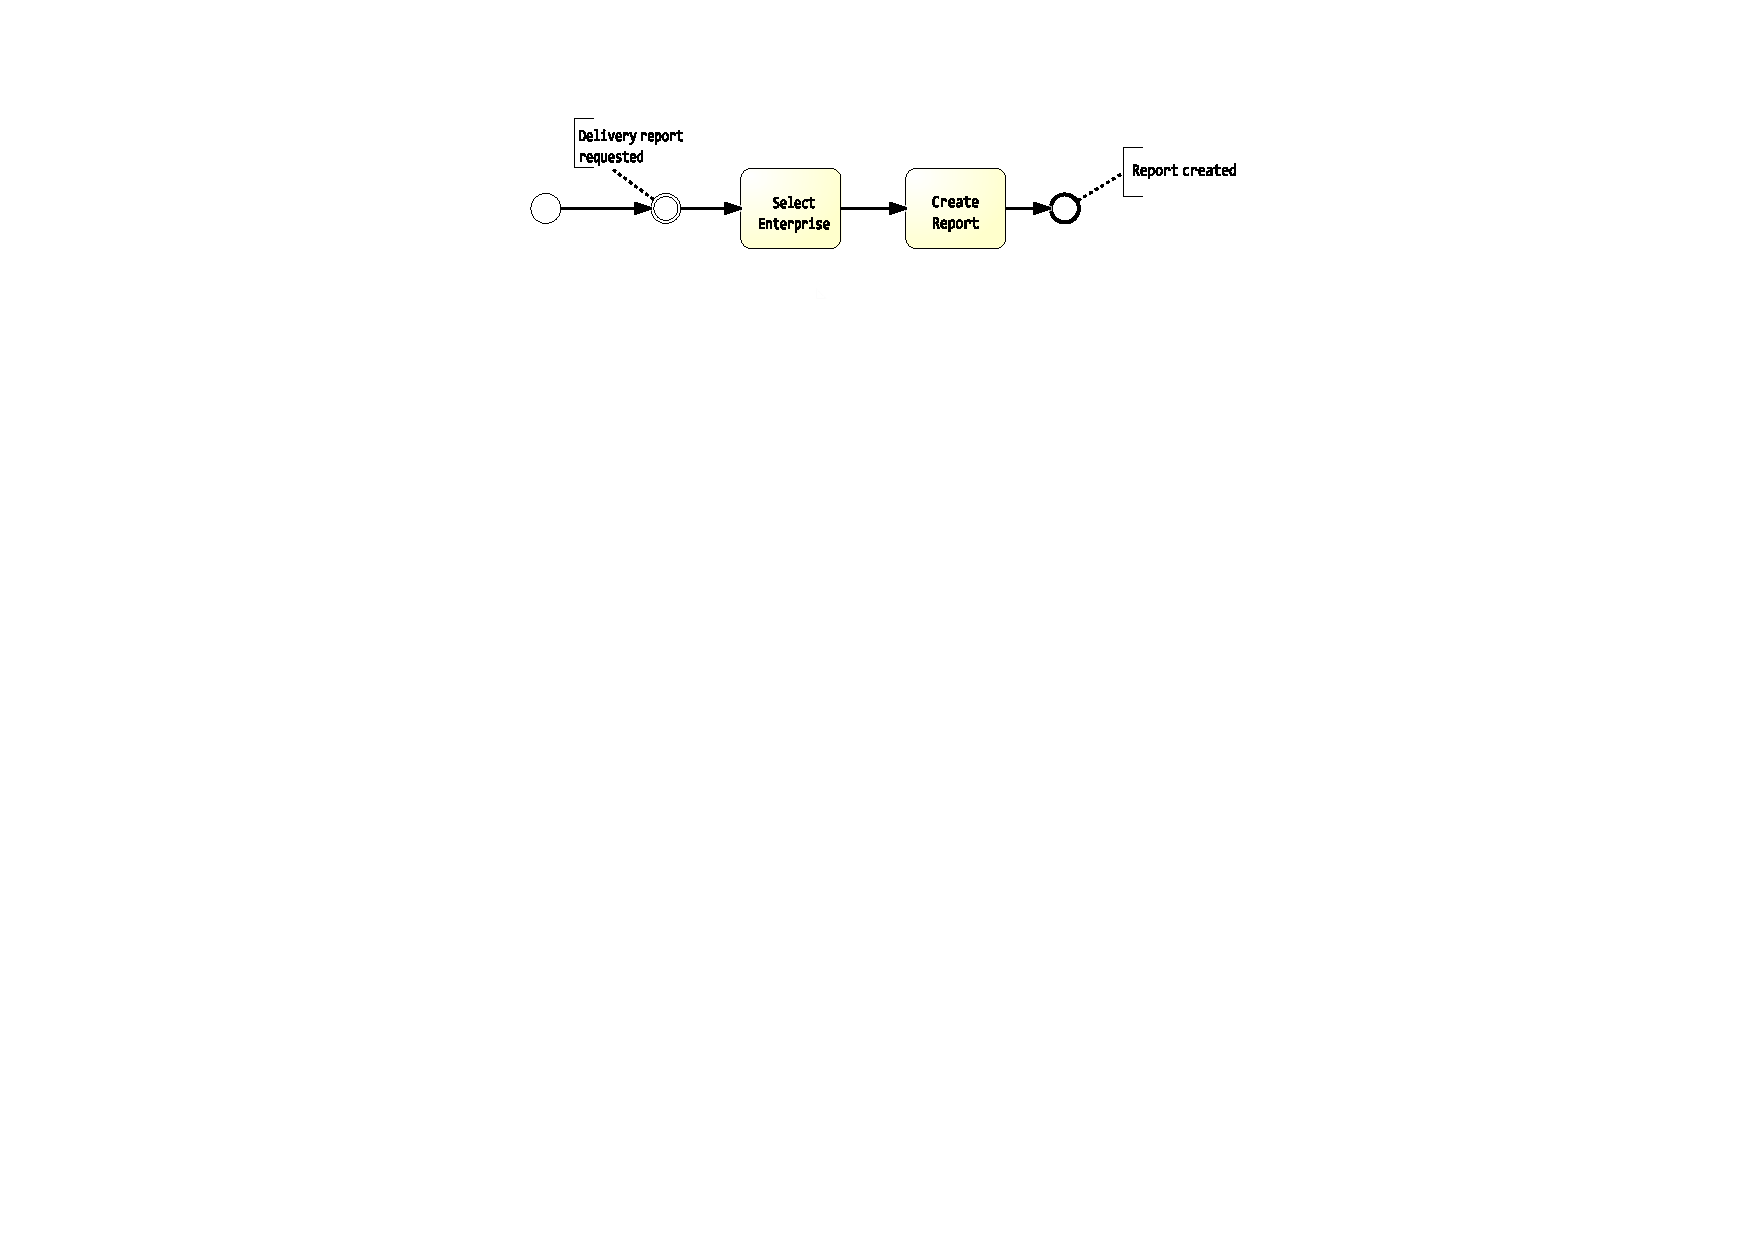
\includegraphics[width=\textwidth, trim={6cm 16.5cm 7cm 1cm}]{img/UC6Control.pdf}
	\caption{Control Flow UC6 - Show Delivery Reports }
	\label{fig:UC6Control}
\end{figure}

%"l, b, r, t"
\begin{figure}[h!]
	\centering
	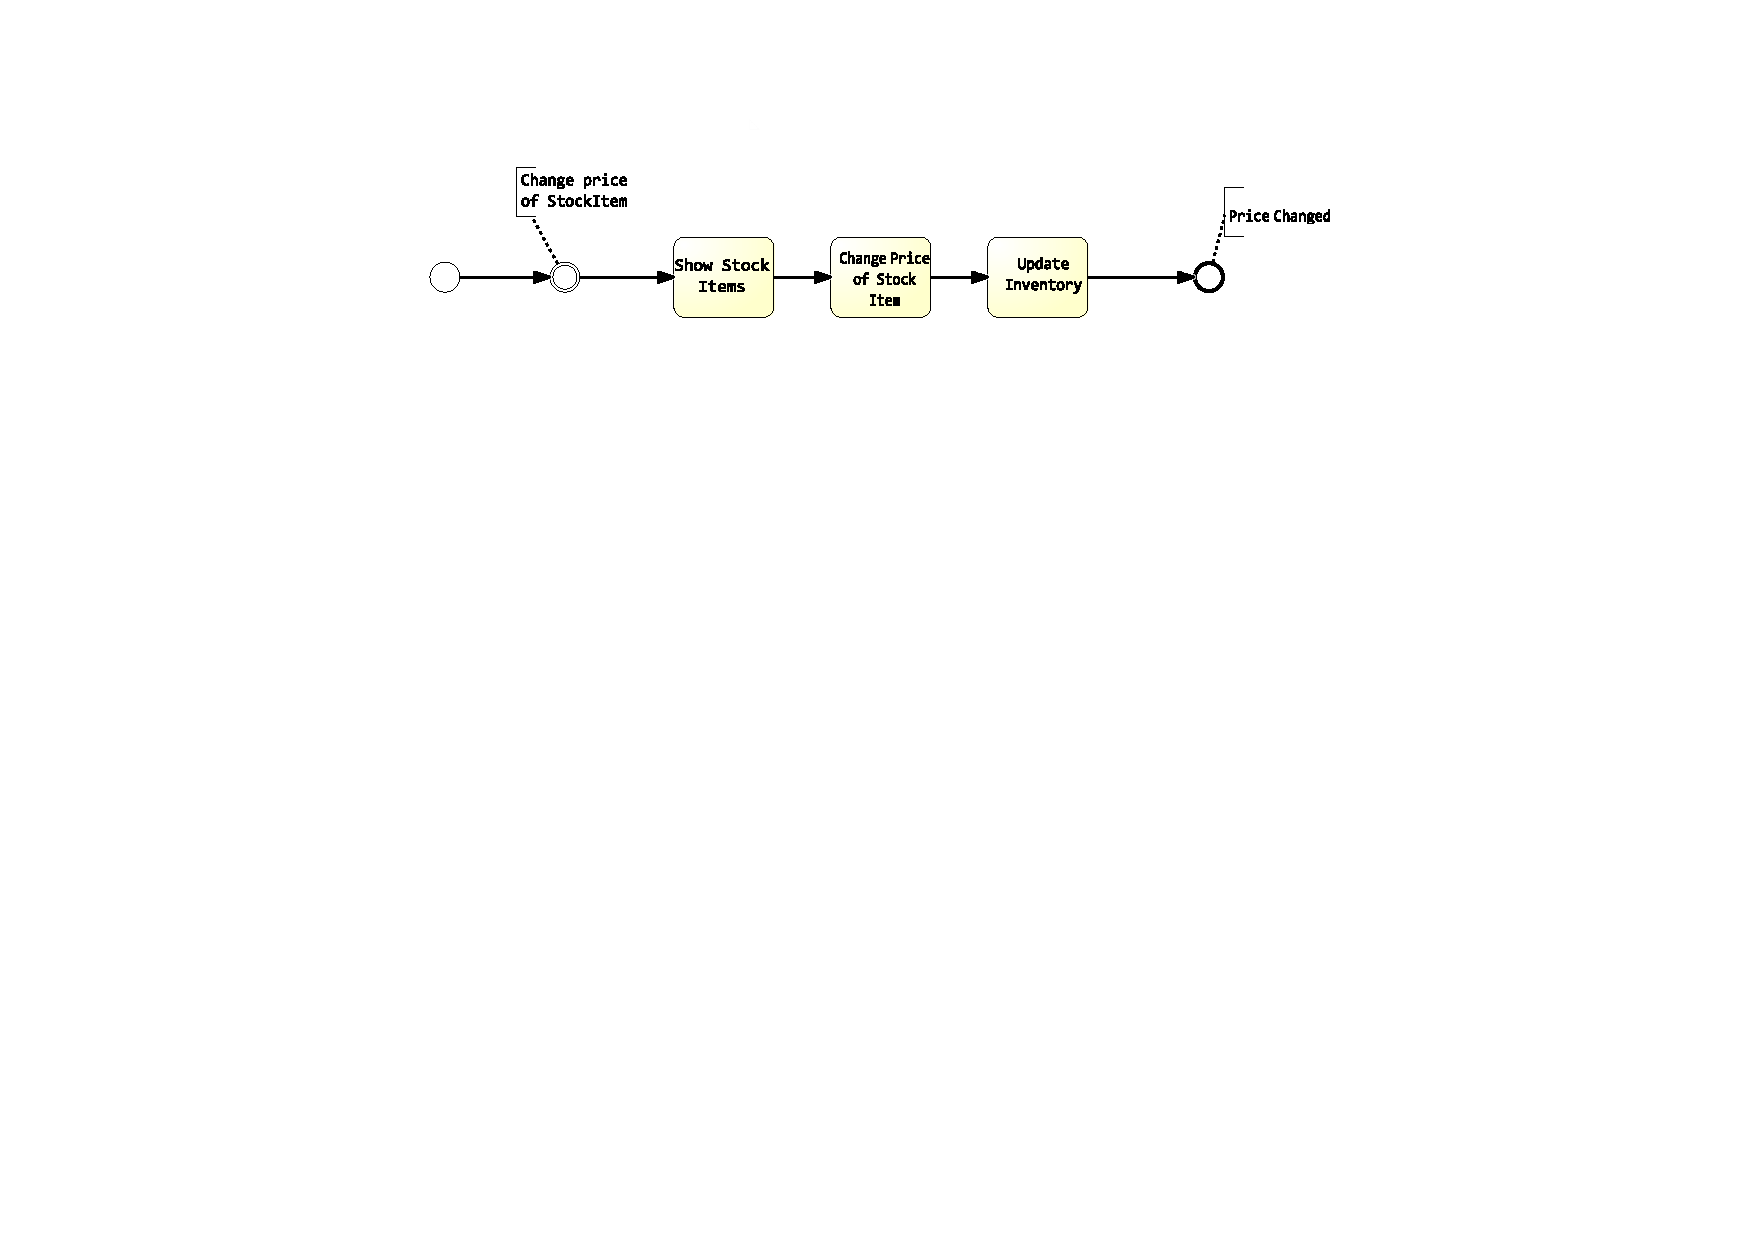
\includegraphics[width=\textwidth, trim={6cm 15.5cm 7cm 1cm}]{img/UC7Control.pdf}
	\caption{Control Flow UC7 - Change Price }
	\label{fig:UC7Control}
\end{figure}


\pagebreak












\section{Data Flow Diagrams}
\label{sec:appendix:DataFlow}

%"l, b, r, t"
\begin{figure}[h!]
	\centering
	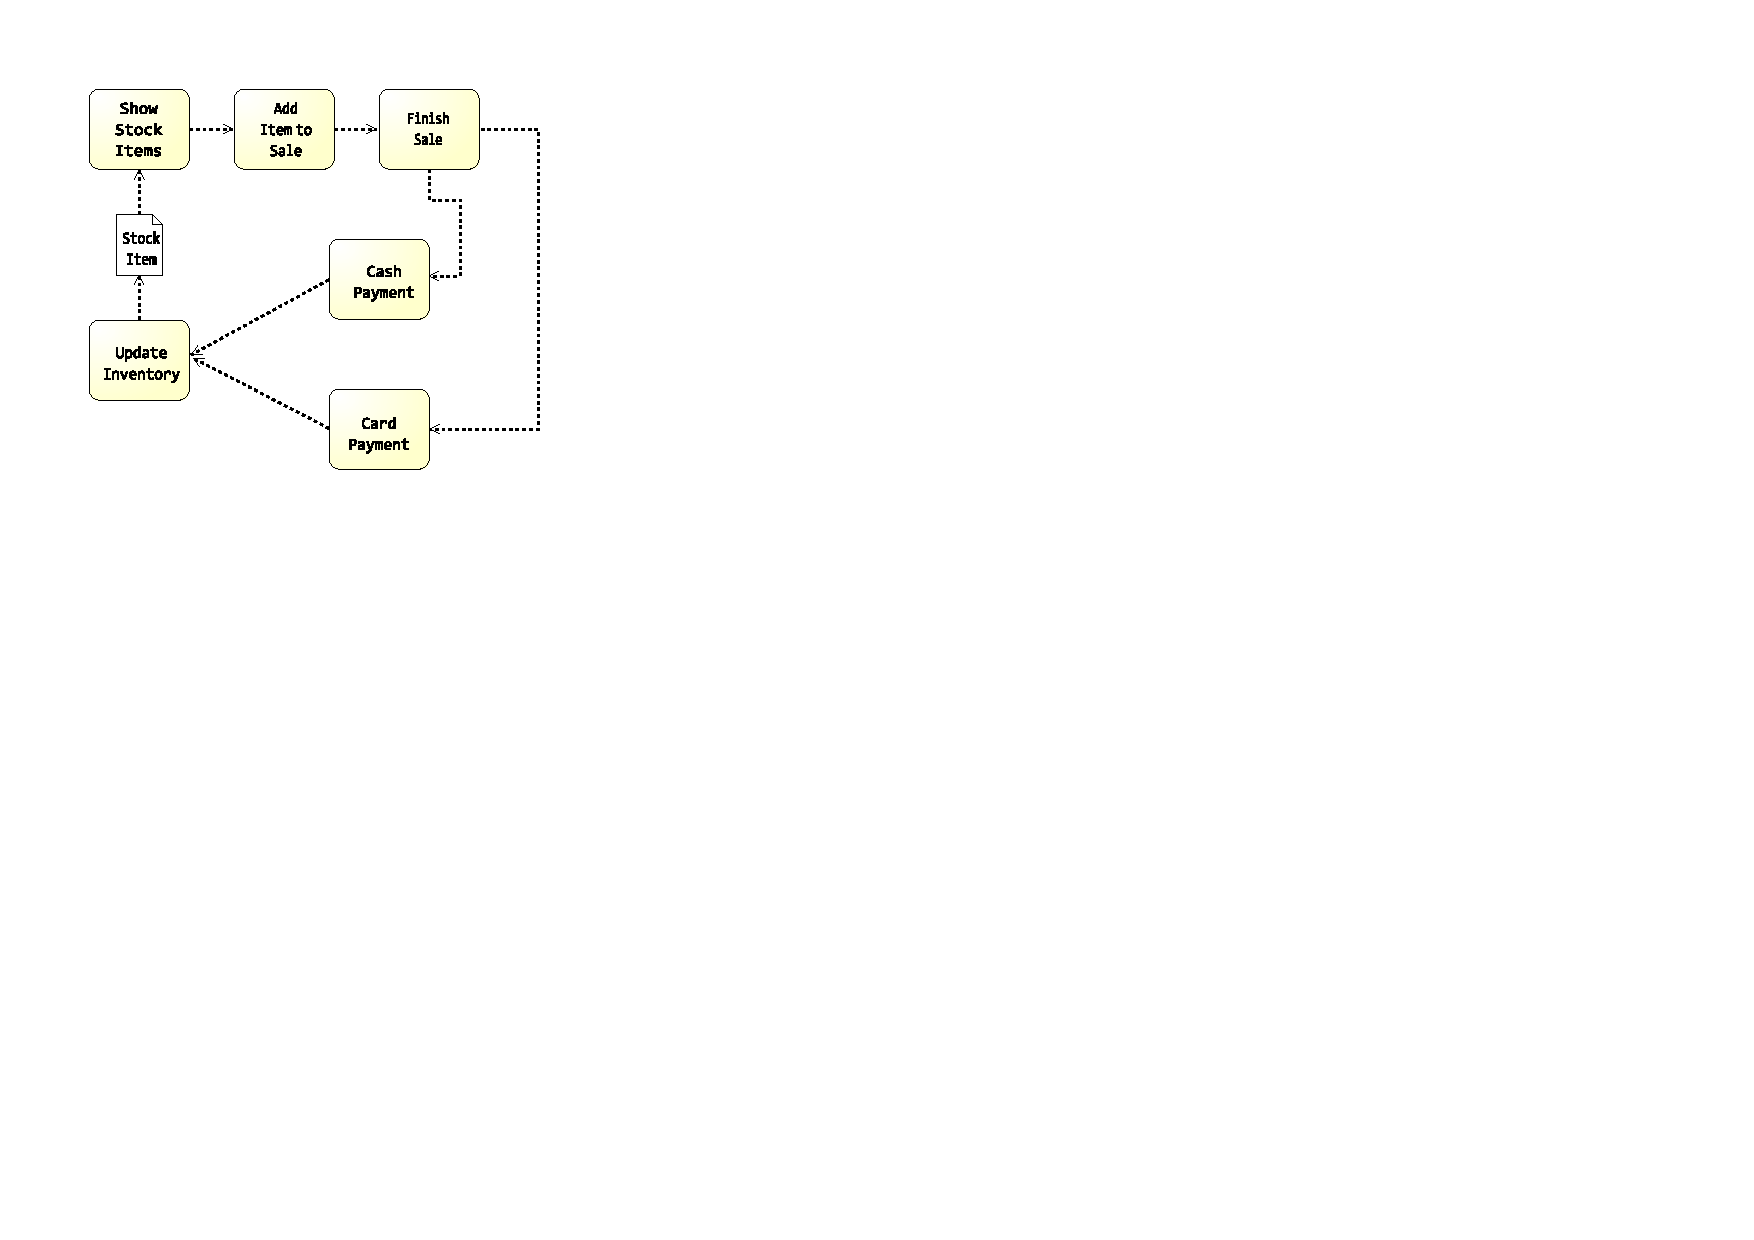
\includegraphics[width=5.5cm, trim={3cm 13cm 22cm 1cm}]{img/UC1DFD.pdf}
	\caption{Data Flow UC1 - Start Sale}
	\label{fig:UC1DFD}
\end{figure}


%"l, b, r, t"
\begin{figure}[h!]
	\centering
	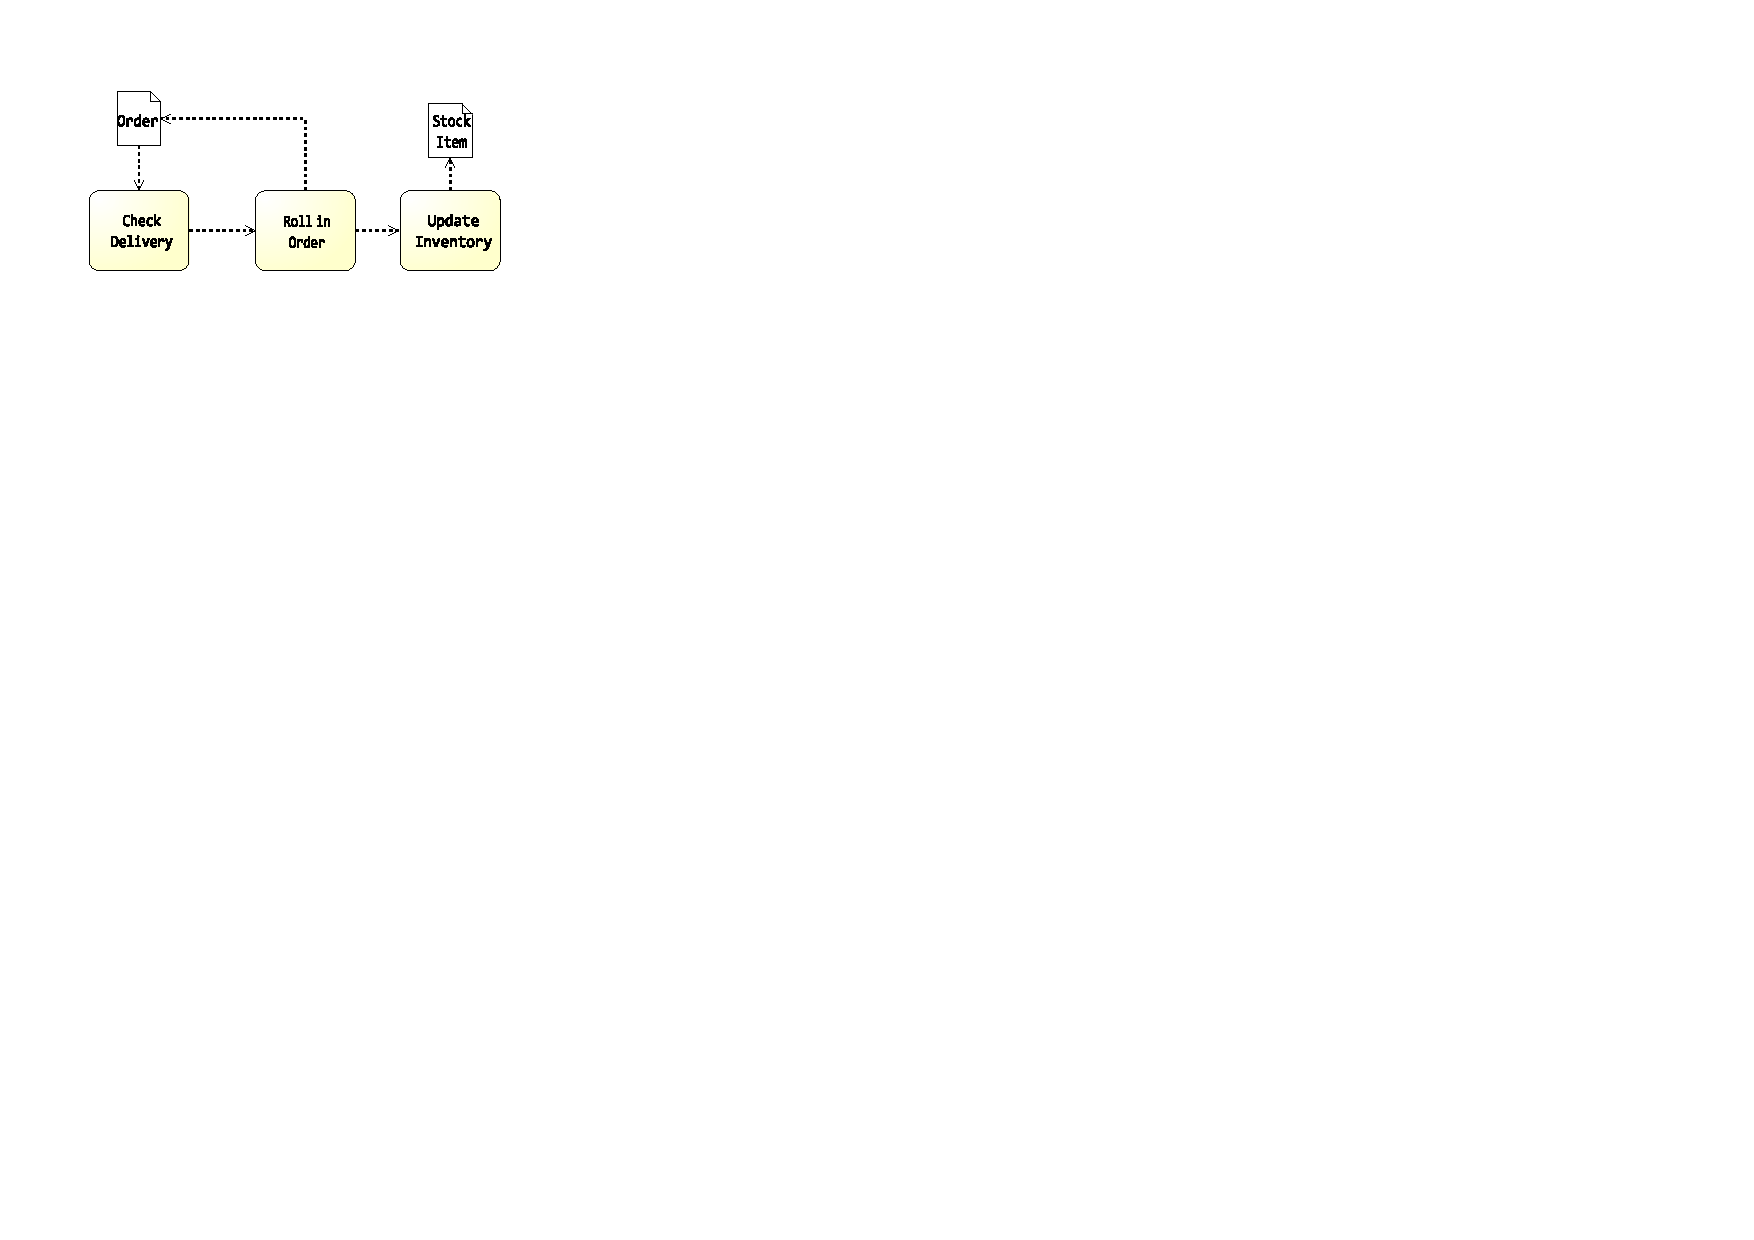
\includegraphics[width=5.5cm, trim={3cm 16cm 22cm 1cm}]{img/UC4DFD.pdf}
	\caption{Data Flow UC4 - Receive Ordered Products }
	\label{fig:UC4DFD}
\end{figure}

\pagebreak

%"l, b, r, t"
\begin{figure}[h!]
	\centering
	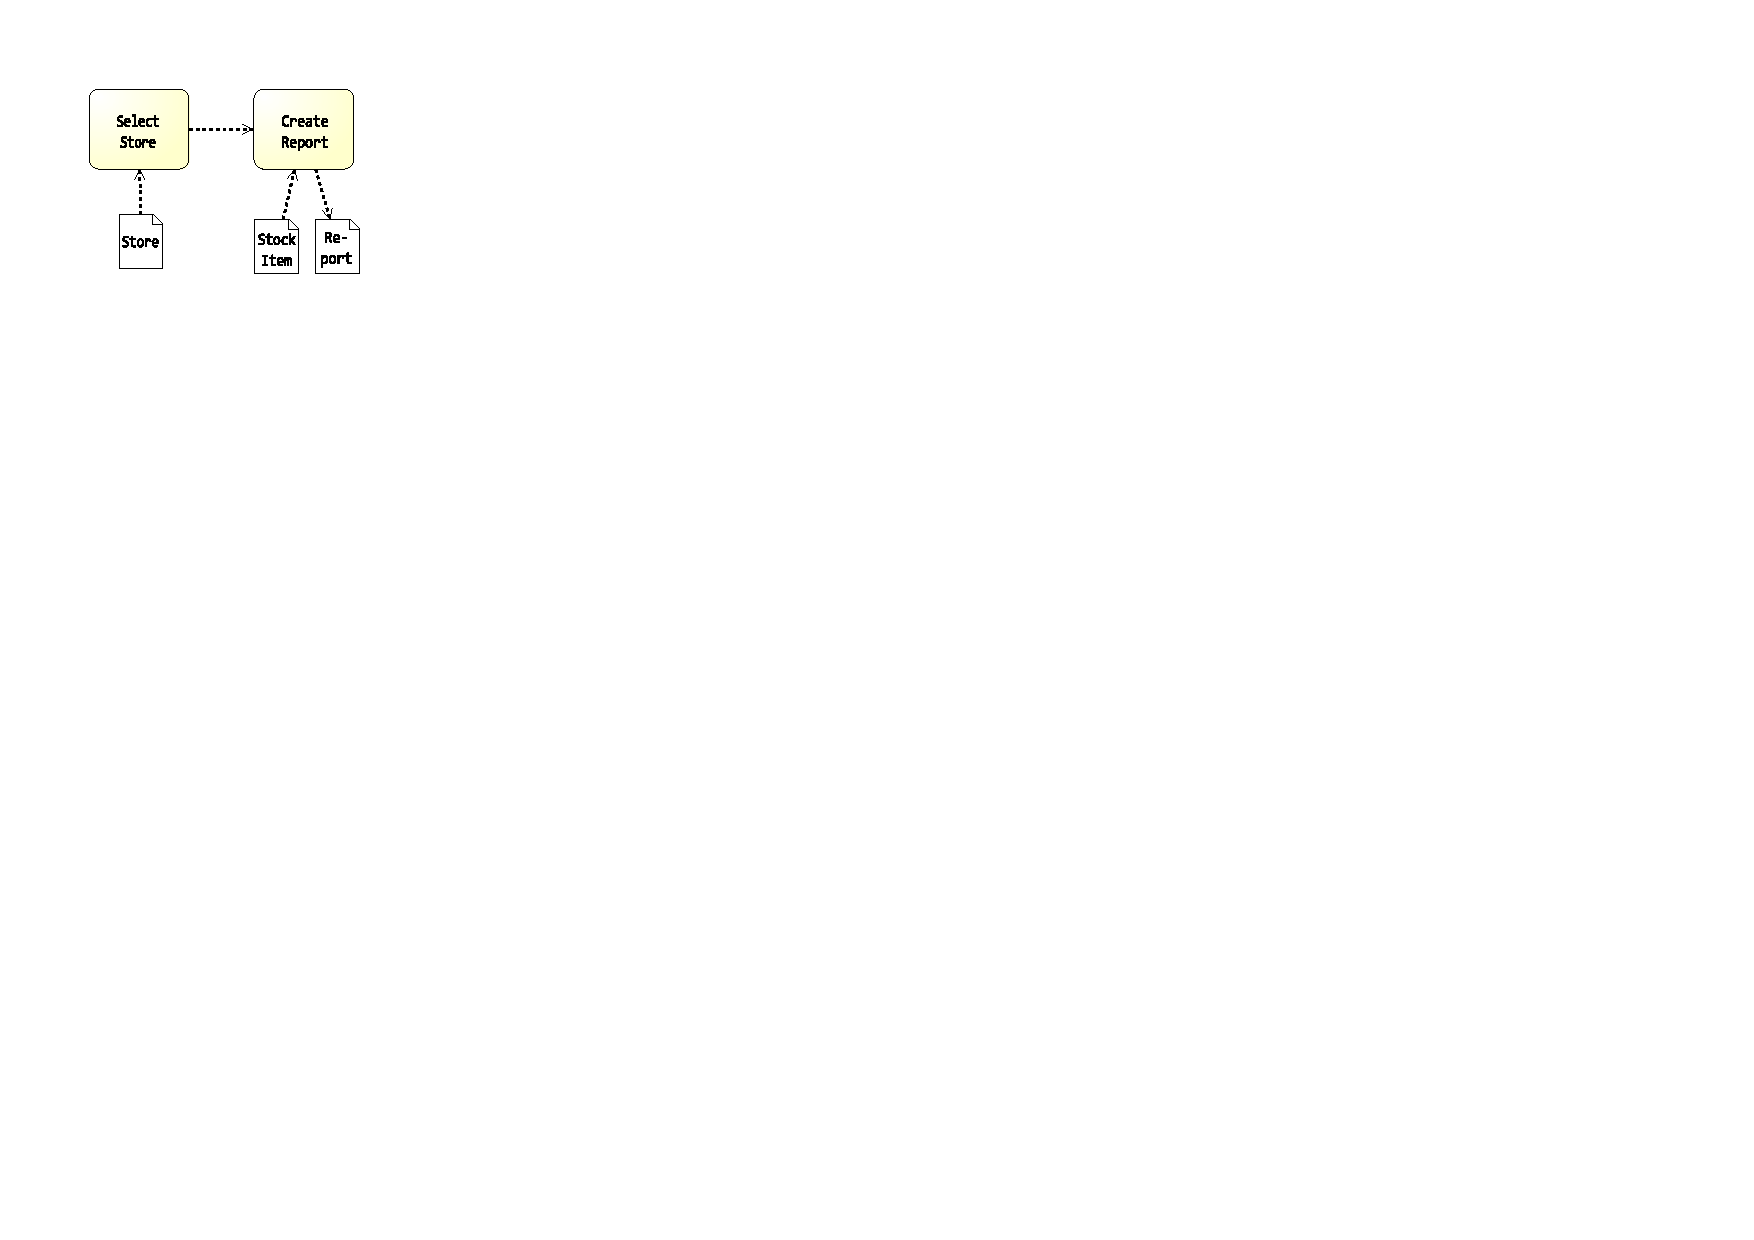
\includegraphics[width=5.5cm, trim={3cm 16cm 22cm 1cm}]{img/UC5DFD.pdf}
	\caption{Data Flow UC5 - Show Stock Reports }
	\label{fig:UC5DFD}
\end{figure}

%"l, b, r, t"
\begin{figure}[h!]
	\centering
	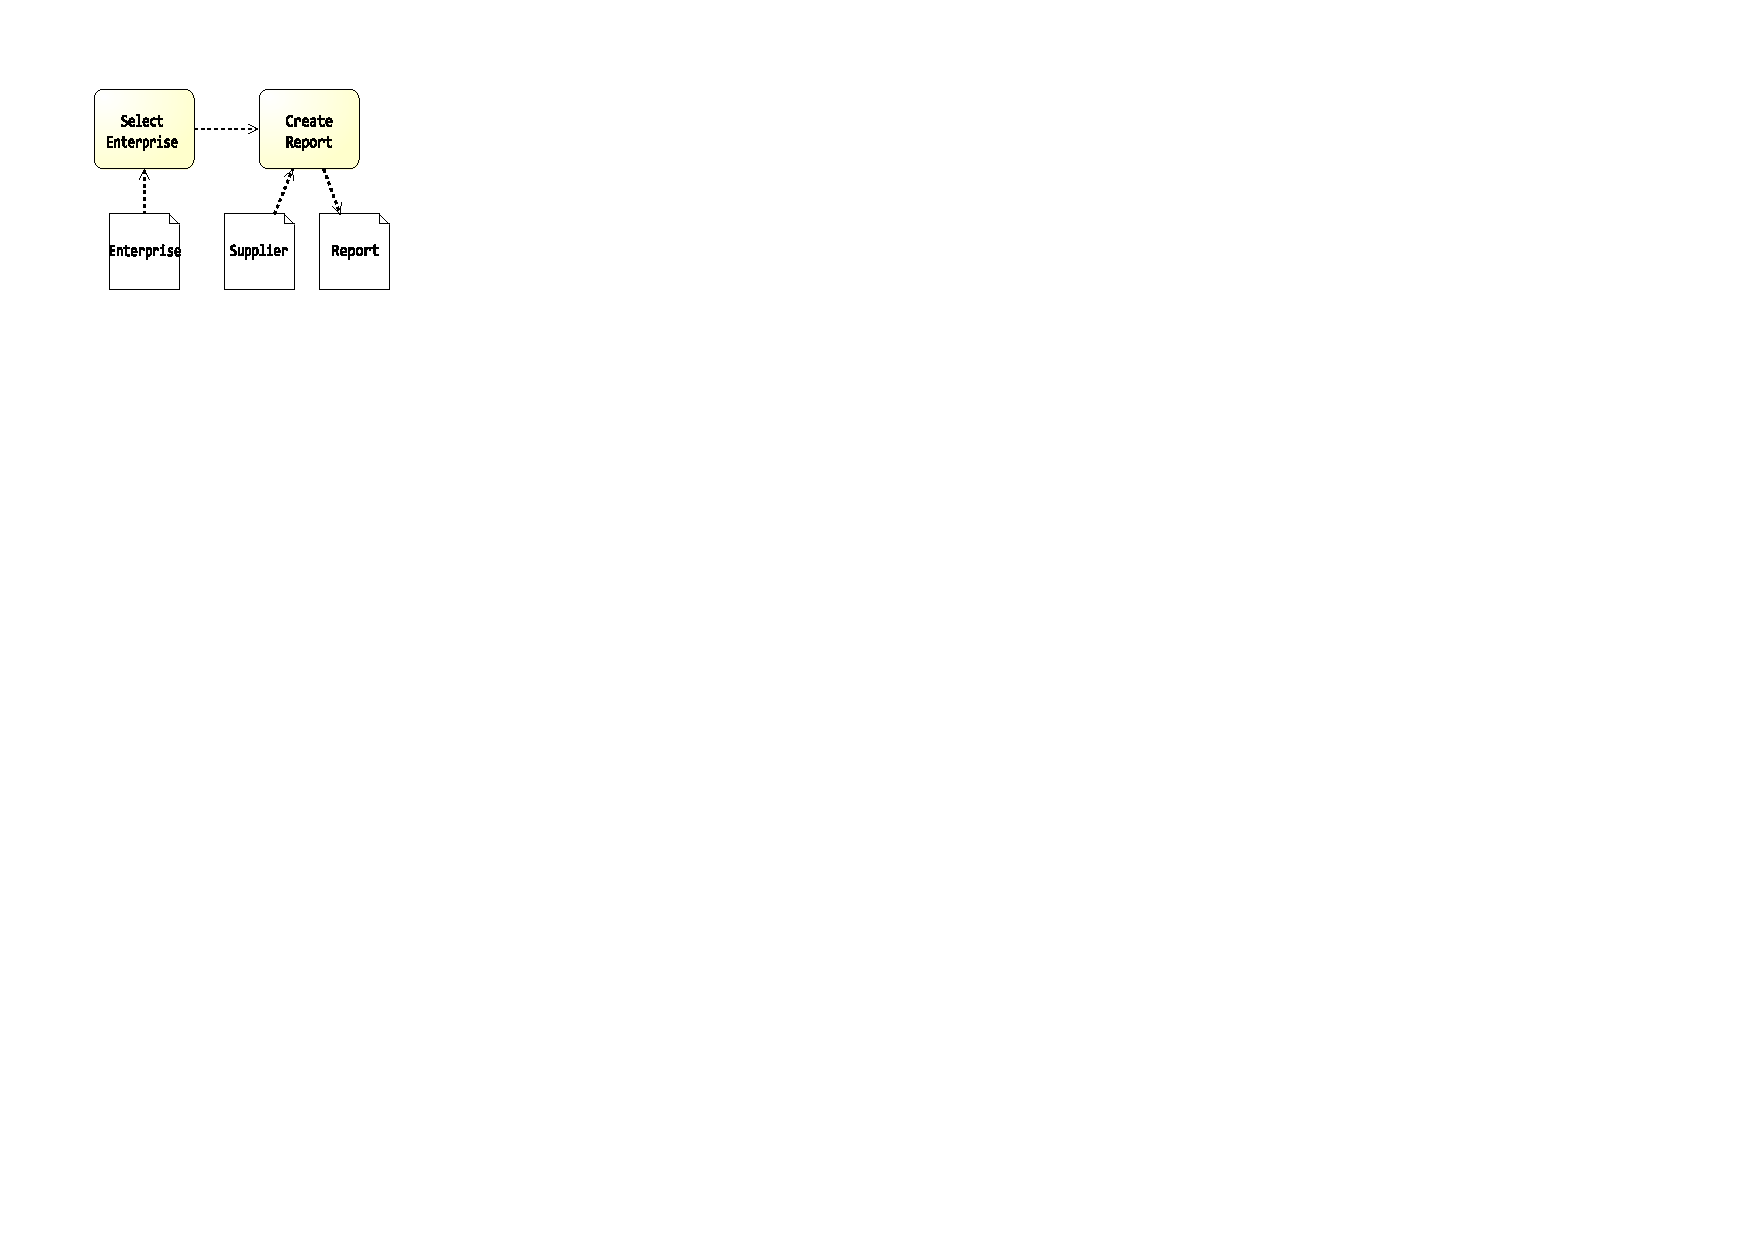
\includegraphics[width=5.5cm, trim={3cm 16cm 22cm 1cm}]{img/UC6DFD.pdf}
	\caption{Data Flow UC6 - Show Delivery Reports }
	\label{fig:UC6DFD}
\end{figure}

%"l, b, r, t"
\begin{figure}[h!]
	\centering
	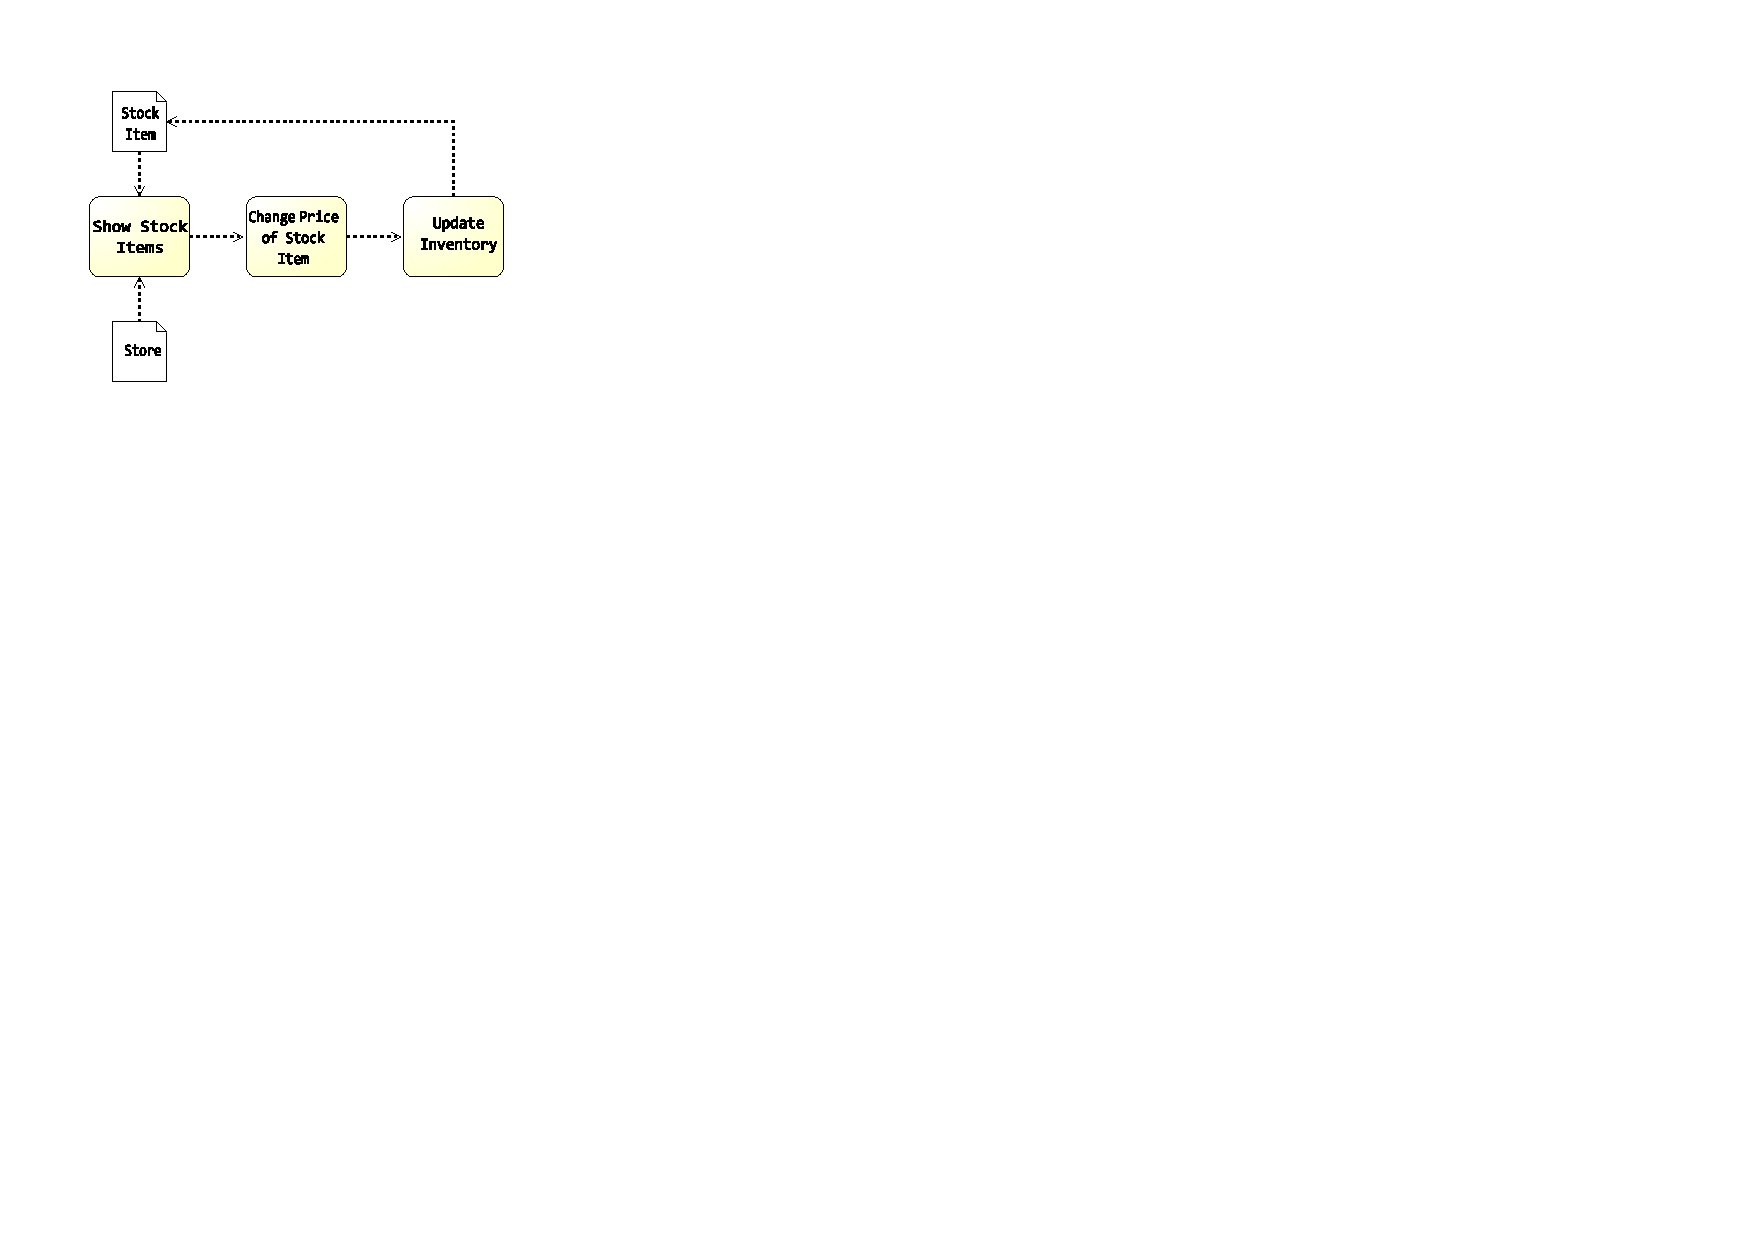
\includegraphics[width=5.5cm, trim={3cm 14.5cm 22cm 1cm}]{img/UC7DFD.pdf}
	\caption{Data Flow UC7 - Change Price }
	\label{fig:UC7DFD}
\end{figure}








\end{document}
